\documentclass[a4paper]{article}
\usepackage[utf8]{inputenc}
\usepackage[english]{babel}
\usepackage{lscape}
\usepackage{booktabs}
\usepackage{graphicx} 
\graphicspath{ {./images/} }
\usepackage{setspace}
\usepackage{upgreek}
\usepackage{ragged2e}
\usepackage{caption}
\captionsetup[table]{justification=centering, singlelinecheck=off}
\usepackage{multirow}
\usepackage[breaklinks]{hyperref}
\usepackage{flafter}
\usepackage{float}
\usepackage{footnote}
\usepackage{afterpage}
\usepackage{caption}
\usepackage{subcaption}
\usepackage{listings}
\usepackage[utf8]{inputenc}
\usepackage{graphicx}
\usepackage{caption}
\usepackage{subcaption}
\usepackage[margin=1.0in]{geometry}
\usepackage[usenames,dvipsnames]{color}
\usepackage{natbib}
\usepackage{amsmath}
\usepackage{booktabs}
\usepackage{dcolumn}
\newcolumntype{d}[1]{D{.}{.}{#1}}
\usepackage[section]{placeins}


\lstset{ 
  language=R,                     % the language of the code
  basicstyle=\small\ttfamily, % the size of the fonts that are used for the code
  numbers=left,                   % where to put the line-numbers
  numberstyle=\small\color{Blue},  % the style that is used for the line-numbers
  stepnumber=1,                   % the step between two line-numbers. If it is 1, each line
                                  % will be numbered
  numbersep=5pt,                  % how far the line-numbers are from the code
  backgroundcolor=\color{white},  % choose the background color. You must add \usepackage{color}
  showspaces=false,               % show spaces adding particular underscores
  showstringspaces=false,         % underline spaces within strings
  showtabs=false,                 % show tabs within strings adding particular underscores
  frame=single,                   % adds a frame around the code
  rulecolor=\color{black},        % if not set, the frame-color may be changed on line-breaks within not-black text (e.g. commens (green here))
  tabsize=2,                      % sets default tabsize to 2 spaces
  captionpos=b,                   % sets the caption-position to bottom
  breaklines=true,                % sets automatic line breaking
  breakatwhitespace=false,        % sets if automatic breaks should only happen at whitespace
  keywordstyle=\color{RoyalBlue},      % keyword style
  commentstyle=\color{YellowGreen},   % comment style
  stringstyle=\color{ForestGreen}      % string literal style
}

%--------------------------------------------------
\begin{document}
\begin{titlepage}    
% Type down your paper title
\title{Conflicting Forces: The role of positive and negative mechanisms in shaping a child's educational outcome}

% Authors
\author{Beatriz Gietner}
\end{titlepage}

\maketitle

\thispagestyle{empty}

\begin{abstract}


 Much has been said about the role that cognition plays in influencing children and young adults' educational outcomes, however, there is a gap in the existing research when it comes to understanding the significance of non-cognitive skills and behaviors in shaping these outcomes. Although conclusions have been mixed, it is clear that multiple factors contribute to students' performance on standardized tests, educational achievements, and future job success. This study aims to elucidate the less-explored non-cognitive factors on children's educational outcomes. Using data from the Growing Up In Ireland longitudinal study, this study aims to contribute to the literature by constructing noncognitive factors based on the questionnaires administered at the household and school levels and then further employing machine learning algorithms based on econometrics techniques to achieve variable selection and dimensionality reduction. Next, I measure the effect of these noncognitive factors in relation to cognitive factors and other variables selected by machine learning algorithms on test scores.

\section{Introduction}

In the modern world, a student's learning journey is closely tied to their environment, where various non-academic factors play a critical role in shaping their academic success. These factors include attitudes and behaviors, which are developed through the various spheres of influence surrounding students, such as their household and school settings. It is essential to tackle the challenge of catering to culturally diverse students with varying abilities and motivations for learning in the 21st century. We cannot merely enroll children in schools; we must ensure they complete the secondary cycle, gaining the knowledge and skills necessary for personal well-being and national development.\\

To understand the factors that determine educational outcomes, we can divide them into two blocks. The first block concerns a student's family background, including socio-economic status, family structure, family resources, and parental involvement, significantly influencing cognitive and noncognitive performance dimensions. The second block of factors relates to school factors and teaching practices. However, research has revealed that only a few studies examine the impact of a student's noncognitive skills on test scores, considering the many relationships a student has with their parents, teachers, and peers. Therefore, it is vital to investigate how noncognitive skills affect a child's educational outcome while considering these relationships.\\

We must recognize the significance of noncognitive factors in a student's academic success. By understanding the complex interplay between a student's environment, family background, and school factors, we can ensure that every child acquires the knowledge and skills necessary for their personal well-being and national development, regardless of their cultural background, abilities or motivations for learning.


\section{Literature review}
\subsection{Education and skills}
Education is, in its nature, multidimensional. It happens in a feedback loop across time and space and concerns many agents and institutions. Because resources such as money and labor are often scarce, they must be allocated wisely. Therefore, it is essential to find ways to get the most significant outcome, given the resources available. One way of measuring the effectiveness of resources that go into educating students is through completed levels and years of education (quantity, educational attainment) and test scores (quality, educational achievement). More properly qualified and skillful students lead better lives and participate more actively in civic duties and the labor market (\citet{oreopoulos2011}). \citet{kautz2014} note that a growing body of empirical research shows that noncognitive skills rival IQ in predicting educational attainment, labor market success, health, and criminality. Not only that, but the literature on the returns to education, both private and social, is vast and almost unanimous on the importance of improving educational outcomes for students. However, to improve educational outcomes, we must understand what goes into these outcomes, what factors contribute to more years of education and better test scores, and how we can measure such factors.\\\

From an economics perspective, a skill is a form of human capital that increases productivity while the market defines its value, and education is perceived as an essential investment in skills development (\cite{zhou2017}). The literature divides skills into two categories: cognitive and noncognitive skills (a term first coined by James Heckman). According to \citet{brunello2011}, there is evidence that high cognitive test scores are likely to result not only from high cognitive skills but also from high motivation and adequate personality traits, which can be considered noncognitive skills in some sense. More persistent students learn more and better. \cite{borghans2008} state that a relationship between noncognitive skills and test scores can exist for two reasons: when there are sufficient rewards involved, people with favorable behavioral or labor-market outcomes might have an attitude to put in effort, and when rewards are not necessary in place, people who are motivated to perform well and who have a positive attitude toward work might be more inclined to do their best at tests. While cognition can be proxied by test scores, test scores do not simply reflect cognitive ability. \citet{duckworth2006}, in a study about the difference in test scores between girls and boys, concluded that because girls had better final grades than boys, even after controlling for measured IQ, they were significantly better at exercising self-discipline during the academic year. \cite{balart2018} used performance decline in PISA test scores as a measure of effort. They found that the effect of cognitive skills was reduced by approximately forty percent in models that control for noncognitive factors.\\\

Noncognitive skills enable people; consequently, greater skill levels foster social inclusion and promote economic and social mobility (\cite{kautz2014}). Perseverance, dependability, and consistency are some of the most important predictors of grades in school, according to \citet{bowles2011}, and they are noncognitive skills. Noncognitive skills can be learned, and they can change over the life cycle. Skill development is a dynamic process in which the early years lay the foundation for successful investment in later years (\cite{kautz2014}). Both cognitive and noncognitive skills have different levels of malleability depending on a child's developmental stage; they can change with age and with instruction: cognitive and noncognitive skills are highly malleable in the early years of a child's life, while noncognitive skills are more malleable than cognitive skills later on, during her adolescent years (\citet{kautz2014}).

\subsection{Defining and measuring skills}

\cite{pandiello} attest that social groups and public authorities ignore noncognitive abilities because of the lack of objective evaluation metrics and the difficulty in establishing standard definitions for the relevant social values. \citet{humphries2017} note that the definition of noncognitive skills varies widely across fields such as Sociology, Psychology, and Economics and within fields of study. Labor economists see non-recognition skills as a second dimension of individual heterogeneity (next to cognitive skills); Education economists broadly categorize those as skills that are not captured by standardized tests (soft skills), and that can be measured by observing behavior. Behavioral economists are divided into two groups: one that sees noncognitive skills as a super-ordinate concept summarizing various specific concepts (i.e., economic preferences such as time and risk preferences), and the other that views them as personality measures (such as the Big Five). This divisiveness is challenging when comparing outcomes due to the different measurement instruments used. \citet{humphries2017} reiterate that the construction of a noncognitive factor greatly influences what is being measured, and consensus on outcome interpretation is difficult due to the different motives behind the research and available data sources.\\\

Noncognitive skills and abilities, unlike cognition, are challenging to define and measure. Currently, there is no systematic global measure of noncognitive skills. However, fortunately, the field has expanded enough, and a wide variety of instruments aimed at assessing these skills and abilities have been created. Using measured behaviors to capture noncognitive skills, for example, is a promising, empirically practical approach, according to \citet{kautz2014}. Personality traits represent relatively persistent dimensions of the overall personality, and some play an important role in increasing productivity-enhancing skills. More broadly, economists often use the term noncognitive skills to account for traits specifically related to human capital outcomes (such as educational and labor market achievements), and in Psychology, personality traits are measured using psychometric constructs (\citet{thiel2013}). Therefore, economists and other social scientists can adapt such constructs to their respective fields of study to measure noncognitive skills.

\section{Methodology}
\subsection{Data}
\subsubsection{Growing Up in Ireland}

The data used in the analysis come from the first three waves of the Child Cohort ('98) of the Growing Up in Ireland (GUI) survey. The GUI is a national longitudinal study of children and young people that has been running since 2006. The study followed the progress of two groups of children: 8,568 9-year-olds (Cohort' 98), representing approximately 14\% of all 9-year-olds in Ireland, and 10,000 9-month-olds (Cohort' 08), for the last fifteen years. Subsequent waves of the '98 cohort saw some drop-off in participation: 7,525 children (87.9\%) in the second wave (2011-2012), 6,216 young adults (72.5\%) in the third wave (2015-2016), and 5,190 young adults (60\%) in the fourth wave (2018-2019). The survey stands out for its large, nationally representative sample and longitudinal nature. The first cohort sample was selected from clustering at the school level, and the second cohort was sampled randomly from the Child Benefit records. The members of Cohort '98 are now 25-26 years old and were interviewed and had their cognitive abilities tested in every wave so far:\\
\begin{itemize}
    \item Wave one at nine years of age in 2007/2008,\\
    \item Wave two at 13 years of age in 2011/2012, and\\
    \item Wave three at 17/18 years of age in 2015/2016.
\end{itemize}   

\subsubsection{Cognitive and noncognitive instrument measurements}

In wave 1, the children were tested in person in Reading and Maths (using the Drumcondra Reading and Maths tests, a set of curriculum-based standardized assessments of reading and maths achievement for primary school pupils in Ireland) and evaluated by their teacher at the school level. In wave 2, their verbal reasoning and numerical abilities were tested (using the Drumcondra Verbal Reasoning and Numerical Ability tests and the British Ability Scales, one of the leading standardized batteries in the UK for assessing a child's cognitive ability and educational achievement). In wave three, they were asked about Junior and Leaving Cert (if they already sat) results and asked for permission to link to the Central Admissions Office database in the future (if they still need to sit). Their cognitive ability was determined through a composite score derived from three assessments: a verbal fluency test, a vocabulary test, and a set of numeracy tests. The verbal fluency test encompassed two aspects: the FAS score, measuring the number of words generated beginning with F, A, or S in one minute, and the Animal Naming score, gauging the number of animal species named in one minute. The vocabulary test consisted of 20 items, each followed by a list of five words, requiring the selection of the word most closely related in meaning. The numeracy test evaluated performance in basic arithmetic through three mathematical calculations. These measures were combined through principal component analysis, yielding a single component representing cognitive ability, where higher scores indicated more remarkable ability.\\\

Academic achievement at the third wave was assessed via the Junior Certificate Examination, a national exam taken by most Irish children around ages 15-16. Mandatory subjects are Irish, English, Maths, and History, and students can choose up to 10 subjects (with at least four mandatory plus two optional) in the areas of Arts and Humanities, Modern Languages, Sciences, and Applied Sciences. Before 2017 (when the survey took place), grades were given on a scale of A to F across different levels of the exam (Higher, Ordinary, Foundation). The Junior Certificate Examination in Ireland marks the end of three years of studying various subjects. It typically spans two to three weeks of individual subject exams at the end of the school year in June, and a student cannot fail the examination. Regardless of their examination results, all students progress to the next year of education if they wish to do so. The time frame between the Junior Certificate (ages 15-16) and the age range of the GUI wave 3 participants (16-18) was relatively close. Because the Junior Cert syllabus and exam content are predetermined three years in advance, achieving success reflects the culmination of a structured curriculum and learning process. Given this foresight, one would anticipate that specific noncognitive skills are pivotal in shaping outcomes. These skills may include effective planning, adept time management, the ability to prioritize long-term goals over immediate gratification (such as opting to study for an exam well in advance rather than indulging in leisure activities), proficient organization and upkeep of study materials, and judicious allocation of time across a diverse array of academic subjects.\\\

In all four waves of the Child Cohort, the study-child filled out a sixty-item questionnaire on their concept of self based on the Piers-Harris Children's Self-Concept Scale. One of the questionnaire domains (Intellectual and School Status – INT) concerns the child's evaluation of his or her abilities in terms of intellectual and academic tasks. Albeit indirect due to its self-reported nature, it also measures cognitive ability. About personality, one of the dimensions where non-cognition manifests itself (others being through behavioral problems, social skills, communication, self-esteem, persistence, locus of control, empathy, and impulsivity), the study-child was assessed utilizing the Ten Item Personality Inventory (TIPI), a brief instrument designed to assess the five-factor model (FFM) personality dimensions (\citet{thorrisen}). Parent One (primary caregiver - PCG) and Parent Two (secondary caregiver - SCG) completed the scale regarding the study-child in wave three (PCG completed in all three waves). In wave three, the study child also filled out the scale, offering an external and self-assessed gauge of the study child's personality and ensuring consistency. This scale comprises ten items gauging five personality facets: Openness to Experience, Agreeableness, Conscientious, Extraversion, and Neuroticism. Each of the ten items was evaluated on a seven-point scale, from strongly disagree to strongly agree. Each dimension of personality included two statements with two descriptors each. The scores for each measure were derived by summing up both responses and dividing by two according to common practice in the literature (\citet{gosling}). This was done by the GUI researchers and the final score for each item can be found in the AMF files of all waves.\\\

Another dimensionality of emotional characteristics and behaviors covered in the GUI was measured using the Strengths and Difficulties Questionnaire (SDQ), which provides a measure of emotional and behavioral regulation, the Short Mood and Feelings Questionnaire (SMFQ), and the Centre for Epidemiological Studies Depression Scale (CES-D). Apart from all measures of cognitive and noncognitive skills, the questionnaires throughout all waves contain information on a wide range of aspects pertaining to household and school settings, parental incomes and educational achievements, relationships between the study child, her parents (Parenting Style), teachers and peers, attitudes, expectation for the future, health status and hobbies. I have sufficient information to create scales of noncognitive skills by attributing points based on behavioral screening questions.

\subsubsection{AMF versus RMF}

The questionnaire data for all waves of the GUI is divided into two different types according to their availability: the Anonymised Microdata Files (AMF), which are available upon a Data Request Form for Research Purposes through the Irish Social Science Data Archive (ISSDA) website, and the Researcher Microdata Files (RMF), which can only be accessed after a lengthy application process (around eight weeks after the researcher gets appropriately vetted by the Central Statistics Office). Because both the study-child/young adult and her primary and secondary caregiver were assessed on many private topics (such as substance use and mental health disorders), getting access to certain parts of the data requires discretion and a reasonable justification from the researcher. Unfortunately, many other answers were also omitted from the AMF data, such as the exact response to the ten items that compose the TIPI scale and all the items in the SDQ for waves one, two, and three; the choice of college major (by code) and the exact number of points at the Leaving Cert in waves three and four, and the cultural background of the study-child (cultural differences are an essential determinant of noncognitive skills). Many other questions reflect how the study-child's environment contributes to the development of her cognitive and noncognitive skills, such as the level of parental involvement in the study-child's academic life, how far they expect the study-child to go in terms of formal education, how the teacher perceives study-child's skills and abilities in the classroom, the study-child's attitudes towards school, how much time she spends in cognitive-enabling activities such as reading for pleasure. Gathering relevant information and accessing the RMF is still a work in progress.

\subsection{Modelling}

There has been much discussion on the validity of noncognitive factors and instruments for properly assessing noncognitive skills. For example, the Big Five personality inventory (on which the TIPI is based) is not universally accepted, mainly due to its self-reported nature (\cite{duckworth2011}). Many possible variables influence test scores, and these variables are very likely to be correlated. Therefore, we need to account for the presence of multicollinearity. In order to address uncertainties in the model, parameter choice, and the possibility of a strong relationship among the predictor variables, I intend to use algorithmic methods and techniques such as random forest, Ridge, and LASSO. These methods are designed to reduce the dimension of a feature space by minimizing the relationships between variables to decrease the chances of over-fitting a model.\\\

Random forest is a machine learning technique that builds numerous decision trees during training. It combines the predictions from each tree to determine the most frequent class (for classification tasks) or the average prediction (for regression tasks). The algorithm constructs each decision tree using a random subset of the training data and a random subset of features, which helps prevent overfitting and enhances the model's accuracy and reliability.\\\

Ridge regression, a type of linear regression, is a machine learning algorithm used for predictive modeling. It works by adding a penalty term to the standard linear regression objective function, which is proportional to the square of the magnitude of the coefficients. This penalty term, controlled by a hyperparameter called the regularization parameter (or lambda), helps shrink the coefficients to zero, effectively reducing their impact on the model. Ridge regression is commonly employed to mitigate overfitting and improve the model's generalization performance. Lasso regression is similar to ridge regression; it adds a penalty term to the standard linear regression objective function. However, unlike ridge regression, Lasso adds a penalty proportional to the absolute value of the coefficients instead of their squares. This penalty encourages sparse solutions by shrinking some coefficients to precisely zero, effectively performing feature selection. Ridge regression uniformly decreases all coefficients by a modest extent, whereas Lasso regression has the capability to heavily shrink certain features, potentially eliminating them. Ridge and Lasso regression are widely adopted algorithms, with Ridge commonly employed to mitigate overfitting and Lasso utilized for feature selection. Both techniques serve as regularization methods in machine learning. Lasso regression is particularly useful when dealing with high-dimensional datasets with many features, as it helps to identify the most relevant predictors while discarding the less important ones.\\\

The starting point of the modelling process is 

\begin{equation}
y = X \beta+\varepsilon, \quad \mathcal{E} \sim N\left(0, \sigma^2 I\right)
\end{equation}

where $X$ is an $N \times q$ matrix of regressors that may or may not be included in the final model, and $\beta$ $(q \times 1)$ contains the parameters to be estimated.

\subsection{Variables}


\begin{gather*}
\text{JCGrade}_{i,j} = \beta_{0} + \beta_{1}\mathbf{TIPIScore}_{i,k,w} + \beta_{2}\mathbf{FamilyCharacteristics}_{i,k,w} \\
+ \beta_{3}\mathbf{SchoolCharacteristics}_{i,w} + \beta_{4}\mathbf{ParentalInvolvement}_{i,k,w} + \beta_{5}\mathbf{PiersHarris}_{i,w} \\
+ \beta_{6}\mathbf{SDQ}_{j,w} + \beta_{7}\mathbf{CognitiveSkills}_{i,l,w} + \varepsilon_{i,j,k,l,w}
\end{gather*}


where $_{i}$ denotes observation for study-child $_{i}$, $_{j}$ denotes the Junior Cert subject, \textit{JCGrade} represents the grade for each Junior Cert subject $_{j}$, \textbf{\textit{TIPIScore}} is a vector containing the final scores for each of the five-item personality dimensions (Openness, Emotional ability, Conscientious, Extrovert, Agreeable) according to study-child $_{i}$ and parent $_{j}$ (PCG, SCG), \textbf{\textit{FamilyCharacteristics}} denotes a vector containing specific measures (such as education and income) for study-child $_{i}$ with parent $_{j}$ in wave $_{w}$, \textbf{\textit{SchoolCharacteristics}} denotes a vector containing information on type of school, DEIS status, and others, for study-child $_{i}$ in wave $_{w}$, \textbf{\textit{ParentalInvolvement}} denotes a vector of six-measures of parental involvement according to study-child $_{i}$ and parent $_{j}$ in wave $_{w}$, \textbf{\textit{PiersHarris}} represents a vector consisting of a series of statements about different aspects of the "self", reported by study-child $_{i}$ in wave $_{w}$, \textbf{\textit{SDQ}} represents a vector of measures that assess emotional and behavioral problems and strengths by parent $_{j}$ on study-child in wave $_{w}$,  \textbf{\textit{CognitiveSkills}} is a vector denoting measures of cognitive skills (such as the results from the Drumcondra tests) of study-schild $_{i}$ in wave $_{w}$, and lastly, $\varepsilon_{i,j,k,l,w}$ represents the error term associated with all the measures in the model.\\\


 As a first approximation, I take the TIPI scores on the five personality dimensions (Openness, Agreeable, Emotional stability, Extravert, Conscientious) self-reported by the primary caregiver (PCG) in waves two and three, the secondary caregiver (SCG) in wave three, and the self-reported scores by study-child in wave three, and regress the Junior Cert grades (grades range from A to E or lower, where A = 5 and E or lower = 1) for six of the Junior Cert subjects on them, without considering Level (Ordinary or Higher). Subjects are considered separately at first, and then I add the grades for all six and use only complete-case observations. I also calculate summary statistics for all Junior Cert subjects, TIPI scores by study-child, PCG, and SCG, and correlation coefficients between the five personality dimensions and gender to demonstrate the presence of multicollinearity. TIPI scores are directly taken from the GUI datasets (they vary from 1 to 7 in intervals of 0.5 - the higher the score, the higher the study-child ranks according to each category). I then add a control variable for gender (male = 1, no specific reason). Further regressions include more explanatory variables such as parental education and school characteristics (type of school and DEIS status). I then created a vector of six measures of parental involvement based on questions taken from the wave three questionnaires. These measures aim to asses how often PCG asks study-child about their performance on exams, how they are getting on with their friends, what are study-child’s plans for the future, how they are getting on with teachers, if they are coping with workload, and lastly, how are they are getting on with subjects at school/college. The scale varies from ”Never or hardly ever” = 1 to ”Several times a week” = 5. The questions can be found in the appendix, where there are also Junior Cert plots for grades for the four mandatory subjects (split by gender), frequency plots for each of the five categories of TIPI scores reported by study-child, PCG, and SCG in waves two and three, and frequency plots for the six measures of parental involvement reported by study-child and PCG in wave three.


\clearpage
\section{Results (preliminary)}
\subsection{Junior Cert grades and TIPI scores}


\subsubsection{Summary statistics}

\begin{table}[!htbp] \centering 
  \caption{Summary statistics - JC Subject grades - Males} 
  \label{} 
\begin{tabular}{@{\extracolsep{5pt}}lccccc} 
\\[-1.8ex]\hline 
\hline \\[-1.8ex] 
Subject & \multicolumn{1}{c}{N} & \multicolumn{1}{c}{Mean} & \multicolumn{1}{c}{St. Dev.} & \multicolumn{1}{c}{Min} & \multicolumn{1}{c}{Max} \\ 
\hline \\[-1.8ex] 
English & 2,792 & 3.370 & 0.898 & 1 & 5 \\ 
Maths & 2,794 & 3.476 & 0.983 & 1 & 5 \\ 
Irish & 2,613 & 3.370 & 0.900 & 1 & 5 \\ 
History & 2,654 & \textbf{3.595} & 1.038 & 1 & 5 \\ 
French & 1,674 & 3.278 & 0.991 & 1 & 5 \\ 
Geography & 2,668 & 3.556 & 0.880 & 1 & 5 \\ 
Science & 2,656 & 3.514 & 0.894 & 1 & 5 \\ 
Spanish & 380 & 2.495 & 0.915 & 1 & 4 \\ 
German & 584 & 2.312 & 0.940 & 1 & 4 \\ 
Arts, Craft and Design & 601 & 2.601 & 0.909 & 1 & 4 \\ 
Music & 393 & 2.730 & 0.838 & 1 & 4 \\ 
Home Economics & 203 & 2.547 & 0.772 & 1 & 4 \\ 
Metalwork & 473 & 2.763 & 0.843 & 1 & 4 \\ 
Material Technology & 1,073 & 2.700 & 0.780 & 1 & 4 \\ 
Technology & 238 & 2.571 & 0.877 & 1 & 4 \\ 
Tech Graphs & 981 & 2.694 & 0.938 & 1 & 4 \\ 
Business & 1,739 & 2.601 & 0.804 & 1 & 4 \\ 
Religious Education & 1,294 & 2.630 & 0.834 & 1 & 4 \\ 
CSPE & 2,707 & \textbf{2.894} & 0.833 & 1 & 4 \\ 
\hline \\[-1.8ex] 
\end{tabular} 
\end{table} 

\begin{table}[!htbp] \centering 
  \caption{Summary statistics - JC subject grades - Females} 
  \label{} 
\begin{tabular}{@{\extracolsep{5pt}}lccccc} 
\\[-1.8ex]\hline 
\hline \\[-1.8ex] 
Subject & \multicolumn{1}{c}{N} & \multicolumn{1}{c}{Mean} & \multicolumn{1}{c}{St. Dev.} & \multicolumn{1}{c}{Min} & \multicolumn{1}{c}{Max} \\ 
\hline \\[-1.8ex] 
English & 2,925 & 3.610 & 0.883 & 1 & 5 \\ 
Maths & 2,928 & 3.491 & 0.941 & 1 & 5 \\ 
Irish & 2,794 & 3.604 & 0.857 & 1 & 5 \\ 
History & 2,787 & \textbf{3.632} & 1.027 & 1 & 5 \\ 
French & 1,846 & 3.502 & 0.972 & 1 & 5 \\ 
Geography & 2,810 & 3.536 & 0.942 & 1 & 5 \\ 
Science & 2,703 & 3.588 & 0.876 & 1 & 5 \\ 
Spanish & 467 & 2.666 & 0.936 & 1 & 4 \\ 
German & 634 & 2.715 & 0.883 & 1 & 4 \\ 
Arts, Craft and Design & 1,197 & 2.997 & 0.872 & 1 & 4 \\ 
Music & 863 & 2.849 & 0.787 & 1 & 4 \\ 
Home Economics & 1,740 & 2.924 & 0.738 & 1 & 4 \\ 
Metalwork & 50 & 2.820 & 0.873 & 1 & 4 \\ 
Material Tech & 164 & 2.616 & 0.746 & 1 & 4 \\ 
Technology & 58 & 2.638 & 0.831 & 1 & 4 \\ 
Tech Graphs & 177 & 2.842 & 0.946 & 1 & 4 \\ 
Business & 1,679 & 2.691 & 0.817 & 1 & 4 \\ 
Religious Education & 1,585 & 2.881 & 0.785 & 1 & 4 \\ 
CSPE & 2,857 & \textbf{3.156} & 0.790 & 1 & 4 \\ 
\hline \\[-1.8ex] 
\end{tabular} 
\end{table}


\begin{table}[ht]
\centering
\caption{Comparison of Summary Statistics for JC Subject Grades by gender}
\label{tab:summary_statistics_comparison}
\begin{tabular}{lccccc}
\hline
\hline
Subject & N(M) & N(F) & Mean(St. Dev.)(M) & Mean(St. Dev)(F) & \(\Delta \)Mean(F-M) \\
\hline
English & 2,792 & 2,925 & 3.370(0.898) & 3.610(0.883) & 0.240 \\
Maths & 2,794 & 2,928 & 3.476(0.983) & 3.491(0.941) & 0.015 \\
Irish & 2,613 & 2,794 & 3.370(0.900) & 3.604(0.857) & 0.234 \\
History & 2,654 & 2,787 & \textbf{3.595}(1.038) & \textbf{3.632}(1.027) & 0.037 \\
French & 1,674 & 1,846 & 3.278(0.991) & 3.502(0.972) & 0.224 \\
Geography & 2,668 & 2,810 & 3.556(0.880) & 3.536(0.942) & \textbf{-0.020} \\
Science & 2,656 & 2,703 & 3.514(0.894) & 3.588(0.876) & 0.074 \\
Spanish & 380 & 467 & 2.495(0.915) & 2.666(0.936) & 0.171 \\
German & 584 & 634 & 2.312(0.940) & 2.715(0.883) & 0.403 \\
ACD & 601 & \textbf{1,197} & 2.601(0.909) & 2.997(0.872) & 0.396 \\
Music & 393 & \textbf{863} & 2.730(0.838) & 2.849(0.787) & 0.119 \\
Home Econ. & 203 & \textbf{1,740} & 2.547(0.772) & 2.924(0.738) & 0.377 \\
Metalwork & \textbf{473} & 50 & 2.763(0.843) & 2.820(0.873) & 0.057 \\
Material Tech. & \textbf{1,073} & 164 & 2.700(0.780) & 2.616(0.746) & \textbf{-0.084} \\
Technology & \textbf{238} & 58 & 2.571(0.877) & 2.638(0.831) & 0.067 \\
Tech Graphs & \textbf{981} & 177 & 2.694(0.938) & 2.842(0.946) & 0.148 \\
Business & 1,739 & 1,679 & 2.601(0.804) & 2.691(0.817) & 0.090 \\
Religious Ed. & 1,294 & 1,585 & 2.630(0.834) & 2.881(0.785) & 0.251 \\
CSPE & 2,707 & 2,857 & \textbf{2.894}(0.833) & \textbf{3.156}(0.790) & 0.262 \\
\hline
\end{tabular}
\end{table}



\begin{table}[!htbp] 
\centering 
\caption{Summary statistics - TIPI scores YP, wave 3} 
\label{tab:summary_statistics_tipi_yp} 
\begin{tabular}{@{\extracolsep{5pt}}lccccc} 
\\[-1.8ex]\hline 
\hline \\[-1.8ex] 
Variable & \multicolumn{1}{c}{N} & \multicolumn{1}{c}{Mean} & \multicolumn{1}{c}{St. Dev.} & \multicolumn{1}{c}{Min} & \multicolumn{1}{c}{Max} \\ 
\hline \\[-1.8ex] 
Agreeable & 6,019 & 4.681 & 1.062 & 1.000 & 7.000 \\ 
Conscientious & 6,019 & 5.199 & 1.169 & 1.000 & 7.000 \\ 
Emot. stability & 6,019 & 4.748 & 1.351 & 1.000 & 7.000 \\ 
Extravert & 6,019 & 4.770 & 1.334 & 1.000 & 7.000 \\ 
Openness & 6,019 & \textbf{5.505} & 1.010 & 1.000 & 7.000 \\ 
\hline \\[-1.8ex] 
\end{tabular} 
\end{table}


\begin{table}[!htbp] \centering 
  \caption{Summary statistics - TIPI scores YP, wave 3 (Males)} 
  \label{} 
\begin{tabular}{@{\extracolsep{5pt}}lccccc} 
\\[-1.8ex]\hline 
\hline \\[-1.8ex] 
Variable & \multicolumn{1}{c}{N} & \multicolumn{1}{c}{Mean} & \multicolumn{1}{c}{St. Dev.} & \multicolumn{1}{c}{Min} & \multicolumn{1}{c}{Max} \\ 
\hline \\[-1.8ex] 
Male & 2,835 & 1.000 & 0.000 & 1 & 1 \\ 
Agreeable & 2,835 & 4.509 & 1.046 & 1.000 & 7.000 \\ 
Conscientious & 2,835 & 5.113 & 1.170 & 1.000 & 7.000 \\ 
Emot. stability & 2,835 & 5.145 & 1.247 & 1.000 & 7.000 \\ 
Extravert & 2,835 & 4.750 & 1.330 & 1.000 & 7.000 \\ 
Openness & 2,835 & \textbf{5.472} & 1.023 & 1.500 & 7.000 \\ 
\hline \\[-1.8ex] 
\end{tabular} 
\end{table} 

\begin{table}[!htbp] \centering 
  \caption{Summary statistics - TIPI scores YP, wave 3 (Females)} 
  \label{} 
\begin{tabular}{@{\extracolsep{5pt}}lccccc} 
\\[-1.8ex]\hline 
\hline \\[-1.8ex] 
Variable & \multicolumn{1}{c}{N} & \multicolumn{1}{c}{Mean} & \multicolumn{1}{c}{St. Dev.} & \multicolumn{1}{c}{Min} & \multicolumn{1}{c}{Max} \\ 
\hline \\[-1.8ex] 
Female & 2,978 & 2.000 & 0.000 & 2 & 2 \\ 
Agreeable & 2,978 & 4.848 & 1.048 & 1.000 & 7.000 \\ 
Conscientious & 2,978 & 5.283 & 1.156 & 1.000 & 7.000 \\ 
Emot. stability & 2,978 & 4.380 & 1.339 & 1.000 & 7.000 \\ 
Extravert & 2,978 & 4.788 & 1.327 & 1.000 & 7.000 \\ 
Openness & 2,978 & \textbf{5.536} & 0.993 & 1.000 & 7.000 \\ 
\hline \\[-1.8ex] 
\end{tabular} 
\end{table} 

\begin{table}[!htbp] \centering 
  \caption{\(\Delta \)TIPI scores means between Females and Males, YP, wave 3} 
  \label{} 
\begin{tabular}{@{\extracolsep{5pt}}lcc} 
\\[-1.8ex]\hline 
\hline \\[-1.8ex] 
Variable & Difference in Means \\ 
\hline \\[-1.8ex] 
Agreeable & \textbf{0.339} \\ 
Conscientious & 0.170 \\ 
Emotional Stability & \textbf{-0.765} \\ 
Extravert & 0.038 \\ 
Openness & 0.064 \\ 
\hline \\[-1.8ex] 
\end{tabular} 
\end{table} 





\begin{table}[!htbp] \centering 
 \caption{Summary statistics - TIPI scores, PCG on YP, wave 3} 
  \label{} 
\begin{tabular}{@{\extracolsep{5pt}}lccccc} 
\\[-1.8ex]\hline 
\hline \\[-1.8ex] 
Variable & \multicolumn{1}{c}{N} & \multicolumn{1}{c}{Mean} & \multicolumn{1}{c}{St. Dev.} & \multicolumn{1}{c}{Min} & \multicolumn{1}{c}{Max} \\ 
\hline \\[-1.8ex] 
Agreeable & 5,970 & \textbf{5.712} & 1.192 & 1.000 & 7.000 \\ 
Conscientious & 5,970 & 5.267 & 1.405 & 1.000 & 7.000 \\ 
Emot. stability & 5,970 & 5.330 & 1.410 & 1.000 & 7.000 \\ 
Extravert & 5,970 & 4.757 & 1.524 & 1.000 & 7.000 \\ 
Openness & 5,970 & 5.512 & 1.191 & 1.000 & 7.000 \\ 
\hline \\[-1.8ex] 
\end{tabular} 
\end{table} 

\begin{table}[!htbp] 
\centering
\caption{\(\Delta \)TIPI scores means between Females and Males, PCG on YP, wave 3} 
\begin{tabular}{lccc} 
\hline
\hline 
Variable & Mean PCG on YP (F) & Mean PCG on YP (M) & \(\Delta \)Mean(F-M) \\ 
\hline 
Agreeable & \textbf{5.727} & \textbf{5.701} & 0.026 \\ 
Conscientious & 5.421 & 5.104 & \textbf{0.317} \\ 
Emo. Stability & 5.086 & 5.594 & \textbf{-0.508} \\ 
Extravert & 4.794 & 4.721 & 0.073 \\ 
Openness & 5.619 & 5.399 & 0.220 \\ 
\hline 
\end{tabular} 
\end{table}

\begin{table}[!htbp] \centering 
 \caption{Summary statistics - TIPI scores, SCG on YP, wave 3} 
  \label{} 
\begin{tabular}{@{\extracolsep{5pt}}lccccc} 
\\[-1.8ex]\hline 
\hline \\[-1.8ex] 
Variable & \multicolumn{1}{c}{N} & \multicolumn{1}{c}{Mean} & \multicolumn{1}{c}{St. Dev.} & \multicolumn{1}{c}{Min} & \multicolumn{1}{c}{Max} \\ 
\hline \\[-1.8ex] 
Agreeable  & 3,943 & \textbf{5.616} & 1.202 & 1.000 & 7.000 \\ 
Conscientious  & 3,943 & 5.328 & 1.377 & 1.000 & 7.000 \\ 
Emot. stability  & 3,943 & 5.339 & 1.337 & 1.000 & 7.000 \\ 
Extravert & 3,943 & 4.707 & 1.456 & 1.000 & 7.000 \\ 
Openness  & 3,943 & 5.513 & 1.161 & 1.000 & 7.000 \\ 
\hline \\[-1.8ex] 
\end{tabular} 
\end{table}

\begin{table}[!htbp] 
\centering
\caption{\(\Delta \)TIPI scores means, SCG on YP, wave 3, by gender} 
\begin{tabular}{lccc} 
\hline
\hline 
Variable & Mean SCG on YP (F) & Mean SCG on YP (M) & \(\Delta \)Mean(F-M) \\ 
\hline 
Agreeable & 5.635 & 5.603 & 0.032 \\ 
Conscientious & 5.489 & 5.174 & \textbf{0.315} \\ 
Emo. Stability & 5.133 & 5.553 & \textbf{-0.420} \\ 
Extravert & 4.804 & 4.617 & 0.187 \\ 
Openness & 5.579 & 5.442 & 0.137 \\ 
\hline 
\end{tabular} 
\end{table}


\begin{table}[htbp]
  \centering
  \caption{Correlation between PCG on YP TIPI scores, W2 and W3}
  \begin{tabular}{@{\extracolsep{5pt}}lccccc} 
\\[-1.8ex]\hline 
\hline \\[-1.8ex] 
    Variable & Estimate & P-value \\
    \hline \\[-1.8ex] 
    Agreeable & 0.34 & 1.5e-164$^{***}$ \\
    Conscientious & \textbf{0.39} & 6.4e-213$^{***}$ \\
    Emot. Stability & 0.32 & 4.1e-146$^{***}$ \\
    Extravert & 0.36 & 4.9e-179$^{***}$ \\
    Openness & 0.23 & 5.3e-73$^{***}$ \\
    \hline
  \end{tabular}
    \vspace{0.5em} \\
  \footnotesize Calculated using the Pearson method.
  \footnotesize $^{***}$ \textit{p $<$ 0.001}.
\end{table}

\begin{table}[htbp] \centering 
  \caption{Correlation coefficients for TIPI components and Male} 
  \label{} 
\begin{tabular}{@{\extracolsep{5pt}} ccc} 
\\[-1.8ex]\hline 
\hline \\[-1.8ex] 
 & Estimate & P-value \\ 
\hline \\[-1.8ex] 
Agreeable & $-0.159$ & $0$ \\ 
Conscientious & $-0.073$ & $0$ \\ 
Extravert & $-0.014$ & $0.286$ \\ 
Emot. Stability & \textbf{$0.283$} & $0$ \\ 
Openness & $-0.031$ & $0.017$ \\ 
\hline \\[-1.8ex] 
\end{tabular} 
\end{table}

\begin{table}[htbp]
  \centering
  \caption{Correlation between PCG on YP and YP TIPI scores, W3}
  \begin{tabular}{@{\extracolsep{5pt}}lccccc} 
\\[-1.8ex]\hline 
\hline \\[-1.8ex] 
    Variable & Estimate & P-value \\
    \hline
    Agreeable & 0.24 & 1.1e-80$^{***}$ \\
    Conscientious & 0.42 & 2.5e-254$^{***}$ \\
    Emot. Stability & 0.41 & 1.6e-242$^{***}$ \\
    Extravert & \textbf{0.50} & 0.0e+00$^{***}$ \\
    Openness & 0.29 & 1.9e-112$^{***}$ \\
    \hline
  \end{tabular}
    \vspace{0.5em} \\
  \footnotesize Calculated using the Pearson method.
  \footnotesize $^{***}$ \textit{p $<$ 0.001}.
\end{table}


\begin{table}[htbp]
  \centering
  \caption{Correlation between PCG and SCG on YP TIPI scores, W3}
  \begin{tabular}{@{\extracolsep{5pt}}lccccc} 
\\[-1.8ex]\hline 
\hline \\[-1.8ex] 

    Variable & Estimate & P-value \\
   \hline
    Agreeable & 0.42 & 1.7e-164$^{***}$ \\
    Conscientious & 0.51 & 6.7e-266$^{***}$ \\
    Emot. Stability & 0.47 & 2.1e-215$^{***}$ \\
    Extravert & \textbf{0.53} & 3.8e-279$^{***}$ \\
    Openness & 0.31 & 3.0e-91$^{***}$ \\
    \hline
  \end{tabular}
  \vspace{0.5em} \\
  \footnotesize Calculated using the Pearson method.
  \footnotesize $^{***}$ \textit{p $<$ 0.001}.
\end{table}

\begin{table}[!htbp]
\centering
\caption{Summary Statistics - Total grade - JC}
\label{tab:summary_stats}
\begin{tabular}{lc}
\toprule
Statistic & Value \\
\midrule
Minimum & 10.00 \\
1st Quartile & 19.00 \\
Median & 21.00 \\
Mean & 21.43 \\
3rd Quartile & 24.00 \\
Maximum & 30.00 \\
NAs & 1129 \\
\bottomrule
\end{tabular}
\end{table}

\clearpage
\subsubsection{Regression results}

\begin{table}[!htbp] \centering 
  \caption{Junior Cert grades for the subjects English and Irish, and TIPI scores reported by YP in wave 3} 
  \label{} 
\small 
\begin{tabular}{@{\extracolsep{1pt}}lcccc} 
\\[-1.8ex]\hline 
\hline \\[-1.8ex] 
 & \multicolumn{4}{c}{\textit{Dependent variable:}} \\ 
\cline{2-5} 
\\[-1.8ex] & \multicolumn{2}{c}{English} & \multicolumn{2}{c}{Irish} \\ 
\\[-1.8ex] & YP, wave 3 & YP, wave 3 (male) & YP, wave 3 & YP, wave 3 (male)\\ 
\hline \\[-1.8ex] 
 Agreeable & 0.008 & $-$0.014 & 0.017 & $-$0.006 \\ 
  & (0.011) & (0.012) & (0.011) & (0.012) \\ 
  Conscientious  & \textbf{0.048$^{***}$} & \textbf{0.040$^{***}$} & \textbf{0.054$^{***}$} & \textbf{0.048$^{***}$} \\ 
  & (0.010) & (0.010) & (0.010) & (0.010) \\ 
  Emot. Stability & \textbf{$-$0.034$^{***}$} & $-$0.003 & $-$0.010 & 0.020$^{**}$ \\ 
  & (0.009) & (0.010) & (0.009) & (0.010) \\ 
  Extravert & $-$0.005 & $-$0.016$^{*}$ & $-$0.002 & $-$0.014 \\ 
  & (0.009) & (0.009) & (0.009) & (0.010) \\ 
  Openness  & 0.008 & 0.003 & \textbf{$-$0.056$^{***}$} & $-$0.061$^{***}$ \\ 
  & (0.012) & (0.012) & (0.012) & (0.012) \\ 
  Male &  & \textbf{$-$0.237$^{***}$} &  & \textbf{$-$0.248$^{***}$} \\ 
  &  & (0.025) &  & (0.025) \\ 
  Constant & 3.348$^{***}$ & 3.543$^{***}$ & 3.495$^{***}$ & 3.699$^{***}$ \\ 
  & (0.095) & (0.098) & (0.096) & (0.099) \\ 
 \hline \\[-1.8ex] 
Observations & 5,909 & 5,705 & 5,592 & 5,400 \\ 
R$^{2}$ & 0.006 & 0.021 & 0.009 & 0.027 \\ 
Adjusted R$^{2}$ & 0.005 & 0.020 & 0.008 & 0.026 \\ 
Residual Std. Error & 0.896 (df = 5903) & 0.889 (df = 5698) & 0.883 (df = 5586) & 0.874 (df = 5393) \\ 
F Statistic & \begin{tabular}[t]{@{}c@{}}7.082$^{***}$ \\ (df = 5; 5903)\end{tabular} & \begin{tabular}[t]{@{}c@{}}20.383$^{***}$ \\ (df = 6; 5698)\end{tabular} & \begin{tabular}[t]{@{}c@{}}10.200$^{***}$ \\ (df = 5; 5586)\end{tabular} & \begin{tabular}[t]{@{}c@{}}24.979$^{***}$ \\ (df = 6; 5393)\end{tabular} \\
\hline 
\hline \\[-1.8ex] 
\textit{Note:}  & \multicolumn{4}{r}{$^{*}$p$<$0.1; $^{**}$p$<$0.05; $^{***}$p$<$0.01} \\ 
\end{tabular} 
\end{table} 

\begin{table}[!htbp] \centering 
  \caption{Junior Cert grades for the subjects History and Maths, and TIPI scores reported by YP in wave 3} 
  \label{} 
\small 
\begin{tabular}{@{\extracolsep{1pt}}lcccc} 
\\[-1.8ex]\hline 
\hline \\[-1.8ex] 
 & \multicolumn{4}{c}{\textit{Dependent variable:}} \\ 
\cline{2-5} 
\\[-1.8ex] & \multicolumn{2}{c}{History} & \multicolumn{2}{c}{Maths} \\ 
\\[-1.8ex] & YP, wave 3 & YP, wave 3 (male) & YP, wave 3 & YP, wave 3 (male)\\ 
\hline \\[-1.8ex] 
 Agreeable & $-$0.014 & $-$0.019 & $-$0.013 & $-$0.017 \\ 
  & (0.013) & (0.014) & (0.012) & (0.012) \\ 
  Conscientious & 0.045$^{***}$ & 0.043$^{***}$ & 0.039$^{***}$ & 0.039$^{***}$ \\ 
  & (0.012) & (0.012) & (0.011) & (0.011) \\ 
  Emot. Stability  & 0.029$^{***}$ & 0.037$^{***}$ & 0.024$^{**}$ & 0.030$^{***}$ \\ 
  & (0.011) & (0.011) & (0.010) & (0.010) \\ 
  Extravert  & $-$0.029$^{***}$ & $-$0.033$^{***}$ & $-$0.006 & $-$0.008 \\ 
  & (0.011) & (0.011) & (0.010) & (0.010) \\ 
  Openness & $-$0.052$^{***}$ & $-$0.055$^{***}$ & $-$0.077$^{***}$ & $-$0.078$^{***}$ \\ 
  & (0.014) & (0.015) & (0.013) & (0.013) \\ 
  Male &  & $-$0.072$^{**}$ &  & $-$0.042 \\ 
  &  & (0.030) &  & (0.027) \\ 
  Constant & 3.735$^{***}$ & 3.801$^{***}$ & 3.672$^{***}$ & 3.702$^{***}$ \\ 
  & (0.112) & (0.116) & (0.101) & (0.105) \\ 
 \hline \\[-1.8ex] 
Observations & 5,622 & 5,429 & 5,914 & 5,710 \\ 
R$^{2}$ & 0.008 & 0.009 & 0.009 & 0.010 \\ 
Adjusted R$^{2}$ & 0.007 & 0.008 & 0.009 & 0.009 \\ 
Residual Std. Error & 1.028 (df = 5616) & 1.028 (df = 5422) & 0.958 (df = 5908) & 0.957 (df = 5703) \\ 
F Statistic & \begin{tabular}[t]{@{}c@{}}8.650$^{***}$ \\ (df = 5; 5616)\end{tabular} & \begin{tabular}[t]{@{}c@{}}8.487$^{***}$ \\ (df = 6; 5422)\end{tabular} & \begin{tabular}[t]{@{}c@{}}11.187$^{***}$ \\ (df = 5; 5908)\end{tabular} & \begin{tabular}[t]{@{}c@{}}9.804$^{***}$ \\ (df = 6; 5703)\end{tabular} \\ 
\hline 
\hline \\[-1.8ex] 
\textit{Note:}  & \multicolumn{4}{r}{$^{*}$p$<$0.1; $^{**}$p$<$0.05; $^{***}$p$<$0.01} \\ 
\end{tabular} 
\end{table} 

\begin{table}[!htbp] \centering 
  \caption{Junior Cert grades for the subjects Geography and Science, and TIPI scores reported by YP in wave 3} 
  \label{} 
\small 
\begin{tabular}{@{\extracolsep{1pt}}lcccc} 
\\[-1.8ex]\hline 
\hline \\[-1.8ex] 
 & \multicolumn{4}{c}{\textit{Dependent variable:}} \\ 
\cline{2-5} 
\\[-1.8ex] & \multicolumn{2}{c}{Geography} & \multicolumn{2}{c}{Science} \\ 
\\[-1.8ex] & YP, wave 3 & YP, wave 3 (male) & YP, wave 3 & YP, wave 3 (male)\\ 
 Agreeable  & $-$0.026$^{**}$ & $-$0.027$^{**}$ & $-$0.016 & $-$0.024$^{**}$ \\ 
  & (0.012) & (0.012) & (0.011) & (0.012) \\ 
  Conscientious  & 0.050$^{***}$ & 0.050$^{***}$ & 0.048$^{***}$ & 0.047$^{***}$ \\ 
  & (0.011) & (0.011) & (0.010) & (0.011) \\ 
  Emot. Stability  & 0.035$^{***}$ & 0.040$^{***}$ & 0.021$^{**}$ & 0.036$^{***}$ \\ 
  & (0.009) & (0.010) & (0.009) & (0.010) \\ 
  Extravert  & $-$0.042$^{***}$ & $-$0.047$^{***}$ & $-$0.038$^{***}$ & $-$0.042$^{***}$ \\ 
  & (0.010) & (0.010) & (0.009) & (0.010) \\ 
  Openness  & $-$0.033$^{***}$ & $-$0.032$^{**}$ & $-$0.041$^{***}$ & $-$0.042$^{***}$ \\ 
  & (0.013) & (0.013) & (0.012) & (0.013) \\ 
  Male &  & $-$0.016 &  & $-$0.106$^{***}$ \\ 
  &  & (0.026) &  & (0.026) \\ 
  Constant & 3.626$^{***}$ & 3.630$^{***}$ & 3.682$^{***}$ & 3.736$^{***}$ \\ 
  & (0.098) & (0.102) & (0.097) & (0.100) \\ 
 \hline \\[-1.8ex] 
Observations & 5,656 & 5,466 & 5,532 & 5,348 \\ 
R$^{2}$ & 0.011 & 0.013 & 0.010 & 0.014 \\ 
Adjusted R$^{2}$ & 0.011 & 0.011 & 0.009 & 0.013 \\ 
Residual Std. Error & 0.906 (df = 5650) & 0.907 (df = 5459) & 0.883 (df = 5526) & 0.880 (df = 5341) \\ 
F Statistic & \begin{tabular}[t]{@{}c@{}}13.109$^{***}$ \\ (df = 5; 5650)\end{tabular} & \begin{tabular}[t]{@{}c@{}}11.595$^{***}$ \\ (df = 6; 5459)\end{tabular} & \begin{tabular}[t]{@{}c@{}}11.499$^{***}$ \\ (df = 5; 5526)\end{tabular} & \begin{tabular}[t]{@{}c@{}}12.787$^{***}$ \\ (df = 6; 5341)\end{tabular} \\
\hline 
\hline \\[-1.8ex] 
\textit{Note:}  & \multicolumn{4}{r}{$^{*}$p$<$0.1; $^{**}$p$<$0.05; $^{***}$p$<$0.01} \\ 
\end{tabular} 
\end{table} 


\begin{table}[!htbp] \centering 
  \caption{TIPI scores reported by YP in wave 3, and JC grades} 
  \label{} 
\small 
\begin{tabular}{@{\extracolsep{1pt}}lcc} 
\\[-1.8ex]\hline 
\hline \\[-1.8ex] 
 & \multicolumn{2}{c}{\textit{Dependent variable:}} \\ 
\cline{2-3} 
\\[-1.8ex] & \multicolumn{2}{c}{Total grade - 6 subjects$^1$} \\ 
\\[-1.8ex] & TIPI scores, YP W3 & TIPI scores - male, YP W3\\ 
\hline \\[-1.8ex] 
 Agreeable & $-$0.032 & $-$0.094$^{*}$ \\ 
  & (0.053) & (0.055) \\ 
  Conscientious  & 0.300$^{***}$ & 0.282$^{***}$ \\ 
  & (0.048) & (0.049) \\ 
  Emotional Stability  & 0.022 & 0.124$^{***}$ \\ 
  & (0.043) & (0.046) \\ 
  Extravert & $-$0.150$^{***}$ & $-$0.190$^{***}$ \\ 
  & (0.044) & (0.045) \\ 
  Openness & $-$0.232$^{***}$ & $-$0.253$^{***}$ \\ 
  & (0.058) & (0.059) \\ 
  Male &  & $-$0.768$^{***}$ \\ 
  &  & (0.120) \\ 
  Constant & 21.896$^{***}$ & 22.475$^{***}$ \\ 
  & (0.453) & (0.468) \\ 
 \hline \\[-1.8ex] 
Observations & 4,904 & 4,743 \\ 
R$^{2}$ & 0.014 & 0.024 \\ 
Adjusted R$^{2}$ & 0.013 & 0.023 \\ 
Residual Std. Error & 3.882 (df = 4898) & 3.861 (df = 4736) \\ 
F Statistic & 14.208$^{***}$ (df = 5; 4898) & 19.450$^{***}$ (df = 6; 4736) \\ 
\hline 
\hline \\[-1.8ex] 
\textit{Note:}  & \multicolumn{2}{r}{$^{*}$p$<$0.1; $^{**}$p$<$0.05; $^{***}$p$<$0.01} \\ 
\multicolumn{3}{l}{$^1$: Complete cases: English, History, Irish, Maths, Geography, Science.}\\
\end{tabular} 
\end{table} 



\begin{table}[!htbp] \centering 
  \caption{YP's TIPI scores according to PCG and SCG in waves 2 and 3, and YP's JC grades} 
  \label{} 
\small 
\begin{tabular}{@{\extracolsep{1pt}}lccc} 
\\[-1.8ex]\hline 
\hline \\[-1.8ex] 
 & \multicolumn{3}{c}{\textit{Dependent variable:}} \\ 
\cline{2-4} 
\\[-1.8ex] & \multicolumn{3}{c}{Total grade - 6 subjects$^1$} \\ 
\\[-1.8ex] & PCG on YP, TIPI scores W2 & PCG on YP, TIPI scores W3 & SCG on YP, TIPI scores W3\\ 
\hline \\[-1.8ex] 
 Agreeable & $-$0.044 &  &  \\ 
  & (0.030) &  &  \\ 
  Conscientious  & 0.356$^{***}$ &  &  \\ 
  & (0.028) &  &  \\ 
  Emotional Stability  & 0.077$^{***}$ &  &  \\ 
  & (0.030) &  &  \\ 
  Extravert & $-$0.071$^{**}$ &  &  \\ 
  & (0.028) &  &  \\ 
  Openness & 0.031 &  &  \\ 
  & (0.031) &  &  \\ 
  Agreeable  &  & $-$0.171$^{***}$ &  \\ 
  &  & (0.051) &  \\ 
  Conscientious  &  & 0.622$^{***}$ &  \\ 
  &  & (0.042) &  \\ 
  Emotional Stability  &  & 0.189$^{***}$ &  \\ 
  &  & (0.044) &  \\ 
  Extravert  &  & $-$0.063 &  \\ 
  &  & (0.038) &  \\ 
  Openness  &  & 0.108$^{**}$ &  \\ 
  &  & (0.050) &  \\ 
  Agreeable  &  &  & $-$0.343$^{***}$ \\ 
  &  &  & (0.063) \\ 
  Conscientious  &  &  & 0.630$^{***}$ \\ 
  &  &  & (0.053) \\ 
  Emotional Stability  &  &  & 0.263$^{***}$ \\ 
  &  &  & (0.058) \\ 
  Extravert  &  &  & $-$0.024 \\ 
  &  &  & (0.049) \\ 
  Openness  &  &  & 0.170$^{***}$ \\ 
  &  &  & (0.063) \\ 
  Constant & 19.887$^{***}$ & 17.780$^{***}$ & 18.053$^{***}$ \\ 
  & (0.226) & (0.382) & (0.451) \\ 
 \hline \\[-1.8ex] 
Observations & 4,898 & 4,853 & 3,266 \\ 
R$^{2}$ & 0.040 & 0.057 & 0.061 \\ 
Adjusted R$^{2}$ & 0.039 & 0.056 & 0.059 \\ 
Residual Std. Error & 3.826 (df = 4892) & 3.796 (df = 4847) & 3.790 (df = 3260) \\ 
F Statistic & 41.270$^{***}$ (df = 5; 4892) & 58.909$^{***}$ (df = 5; 4847) & 42.020$^{***}$ (df = 5; 3260) \\ 
\hline 
\hline \\[-1.8ex] 
\textit{Note:}  & \multicolumn{3}{r}{$^{*}$p$<$0.1; $^{**}$p$<$0.05; $^{***}$p$<$0.01} \\ 
\multicolumn{3}{l}{$^1$: Complete cases: English, History, Irish, Maths, Geography, Science.}\\
\end{tabular} 
\end{table}



\begin{table}[!htbp] \centering 
  \caption{YP's TIPI scores according to PCG and SCG in wave 3, and YP's JC grades} 
  \label{} 
\small 
\begin{tabular}{@{\extracolsep{1pt}}lc} 
\\[-1.8ex]\hline 
\hline \\[-1.8ex] 
 & \multicolumn{1}{c}{\textit{Dependent variable:}} \\ 
\cline{2-2} 
\\[-1.8ex] & Total grade - 6 subjects$^1$ \\ 
\\[-1.8ex] & TIPI scores, SCG and PCG on YP W3\\ 
\hline \\[-1.8ex] 
 Agreeable (SCG) & $-$0.302$^{***}$ \\ 
  & (0.067) \\ 
  Conscientious (SCG) & 0.421$^{***}$ \\ 
  & (0.060) \\ 
  Emotional Stability (SCG) & 0.192$^{***}$ \\ 
  & (0.063) \\ 
  Extravert (SCG) & 0.018 \\ 
  & (0.056) \\ 
  Openness (SCG) & 0.136$^{**}$ \\ 
  & (0.064) \\ 
  Agreeable (PCG) & $-$0.167$^{**}$ \\ 
  & (0.066) \\ 
  Conscientious (PCG) & 0.417$^{***}$ \\ 
  & (0.059) \\ 
  Emotional Stability (PCG)& 0.172$^{***}$ \\ 
  & (0.059) \\ 
  Extravert (PCG) & $-$0.082 \\ 
  & (0.053) \\ 
  Openness (PCG) & 0.118$^{*}$ \\ 
  & (0.062) \\ 
  Constant & 16.859$^{***}$ \\ 
  & (0.529) \\ 
 \hline \\[-1.8ex] 
Observations & 3,257 \\ 
R$^{2}$ & 0.082 \\ 
Adjusted R$^{2}$ & 0.080 \\ 
Residual Std. Error & 3.749 (df = 3246) \\ 
F Statistic & 29.159$^{***}$ (df = 10; 3246) \\ 
\hline 
\hline \\[-1.8ex] 
\textit{Note:}  & \multicolumn{1}{r}{$^{*}$p$<$0.1; $^{**}$p$<$0.05; $^{***}$p$<$0.01} \\ 
\multicolumn{2}{l}{$^1$: Complete cases: English, History, Irish, Maths, Geography, Science.}\\
\end{tabular} 
\end{table}


\clearpage
\subsection{Intergenerational education and JC grades}
\subsubsection{Summary statistics}

\begin{table}[htbp]
  \centering
  \caption{Summary Statistics - Demographics, Wave 3}
  \begin{tabular}{@{\extracolsep{5pt}}lccccc} 
\\[-1.8ex]\hline 
\hline \\[-1.8ex] 
    Characteristic & N  (\%) \\
  \hline
    YP gender & N = 5,833 \\
    \hline
    Male & 2,850 (48.9\%) \\
    Female & \textbf{2,983 (51.1\%)} \\
    \hline
    PCG born in Ireland & N = 6,031\\
    \hline
    Yes & \textbf{5,112 (85\%)} \\
    No & 919 (15\%) \\
    \hline
    SCG born in Ireland & N = 3,908 \\
    \hline
    Yes & \textbf{3,363 (86\%)} \\
    No & 545 (14\%) \\
    \hline
    YP born in Ireland & N = 6,032 \\
    \hline
    Yes & \textbf{5,412 (90\%)} \\
    No & 620 (10\%) \\
    \hline
    YP Irish citizen & N = 6,032 \\
    \hline
     Yes & \textbf{5,770 (95.66\%)} \\
     No & 262 (\%4.34 \\
   \hline
  \end{tabular}
\end{table}

\begin{table}[ht]
\centering
\caption{Descriptive Statistics - Intergenerational Education}
\label{tab:descriptive_edu_stats}
\begin{tabular}{@{\extracolsep{5pt}}lccccc} 
\\[-1.8ex]\hline 
\hline \\[-1.8ex] 
Variable & N (\%) & \\
\hline
PCG's highest level of education & N = 5,993\\
\hline
None/Primary school & 126 (2.10\%) \\ 
Lower Secondary & 526 (8.77\%) \\
High Sec/TechVoc/UppSec+Tech/Voc & \textbf{2,219 (37.03\%)} \\
Non Degree & 1,235 (20.60\%) \\
Primary Degree & 1,139 (19.00\%) \\
Postgrad & 744 (12.42\%) \\
\hline
PCG's mother's highest level of education & N = 5,993\\
\hline
Primary level or no formal education & \textbf{2,470 (41.21\%)} \\
Lower secondary (e.g. Junior/Inter Cert) & 1,493 (24.90\%) \\
Upper secondary (e.g. Leaving Cert) & 1,191 (19.86\%) \\
Third level (e.g. Degree or professional qualification) & 711 (11.85\%) \\
\hline
PCG's father's highest level of education & N = 5,993 \\
\hline
Primary level or no formal education & \textbf{2,939 (48.99\%)} \\
Lower secondary (e.g. Junior/Inter Cert) & 1,182 (19.71\%) \\
Upper secondary (e.g. Leaving Cert) & 882 (14.71\%) \\
Third level (e.g. Degree or professional qualification) & 762 (12.71\%) \\
\hline
SCG's highest level of education & N = 3,922 \\
\hline
None/Primary School & 106 (2.70\%) \\
Lower Secondary & 580 (14.78\%) \\
High Sec/TechVoc/UppSec+Tech/Voc & \textbf{1,256 (32.02\%)} \\
Non Degree & 620 (15.81\%) \\
Primary Degree & 796 (20.29\%) \\
Postgrad & 564 (14.38\%) \\
\hline
SCG's mother's highest level of education & N = 3,953 \\
\hline
Primary level or no formal education & \textbf{1,584 (40.10\%)} \\
Lower secondary (e.g. Junior/Inter Cert) & 896 (22.68\%) \\
Upper secondary (e.g. Leaving Cert) & 925 (23.42\%) \\
Third level (e.g. Degree or professional qualification) & 393 (9.95\%) \\
\hline
SCG's father's highest level of education & N = 3,953\\
\hline
Primary level or no formal education & \textbf{1,913 (48.40\%)} \\
Lower secondary (e.g. Junior/Inter Cert) & 750 (18.97\%) \\
Upper secondary (e.g. Leaving Cert) & 611 (15.46\%) \\
Third level (e.g. Degree or professional qualification) & 483 (12.22\%) \\
\hline
\end{tabular}
\end{table}

\clearpage
\subsubsection{Regression results}
\begin{table}[!htbp] \centering 
  \caption{YP's total grade in six subjects (complete cases), and PCG and SCG's educational levels} 
  \label{} 
\small 
\begin{tabular}{@{\extracolsep{1pt}}lcc} 
\\[-1.8ex]\hline 
\hline \\[-1.8ex] 
 & \multicolumn{2}{c}{\textit{Dependent variable:}} \\ 
\cline{2-3} 
\\[-1.8ex] & \multicolumn{2}{c}{Total grade - 6 subjects$^1$} \\ 
\\[-1.8ex] &  PCG's educational level &  SCG's educational level\\ 
\hline \\[-1.8ex] 
 PCG's educational level & 0.841$^{***}$ &  \\ 
  & (0.044) &  \\ 
  SCG's educational level &  & 0.887$^{***}$ \\ 
  &  & (0.048) \\ 
  Constant & 18.132$^{***}$ & 18.301$^{***}$ \\ 
  & (0.180) & (0.199) \\ 
 \hline \\[-1.8ex] 
Observations & 4,867 & 3,251 \\ 
R$^{2}$ & 0.071 & 0.095 \\ 
Adjusted R$^{2}$ & 0.071 & 0.094 \\ 
Residual Std. Error & 3.767 (df = 4865) & 3.722 (df = 3249) \\ 
F Statistic & 371.368$^{***}$ (df = 1; 4865) & 339.392$^{***}$ (df = 1; 3249) \\ 
\hline 
\hline \\[-1.8ex] 
\textit{Note:}  & \multicolumn{2}{r}{$^{*}$p$<$0.1; $^{**}$p$<$0.05; $^{***}$p$<$0.01} \\ 
\multicolumn{3}{l}{$^1$: Complete cases: English, History, Irish, Maths, Geography, Science.}\\
\end{tabular} 
\end{table} 


\begin{table}[!htbp] \centering 
  \caption{YP's total grade in six subjects (complete cases), and PCG's, SCG's and their parents' educational levels} 
  \label{} 
\small 
\begin{tabular}{@{\extracolsep{1pt}}lcc} 
\\[-1.8ex]\hline 
\hline \\[-1.8ex] 
 & \multicolumn{2}{c}{\textit{Dependent variable:}} \\ 
\cline{2-3} 
\\[-1.8ex] & \multicolumn{2}{c}{Total grade - 6 subjects$^1$} \\ 
\\[-1.8ex] & PCG's+SCG's educ. levels & PCG+SCG+their parents' educ. levels\\ 
\hline \\[-1.8ex] 
 PCG's educational level & 0.538$^{***}$ & 0.510$^{***}$ \\ 
  & (0.058) & (0.063) \\ 
  SCG's educational level & 0.688$^{***}$ & 0.596$^{***}$ \\ 
  & (0.052) & (0.057) \\ 
  PCG's father's educ. level &  & 0.028 \\ 
  &  & (0.073) \\ 
  PCG's mother's educ. level &  & 0.061 \\ 
  &  & (0.075) \\ 
  SCG's father's educ. level &  & 0.051 \\ 
  &  & (0.076) \\ 
  SCG's mother's educ. level &  & 0.143$^{*}$ \\ 
  &  & (0.079) \\ 
  Constant & 16.927$^{***}$ & 16.880$^{***}$ \\ 
  & (0.246) & (0.271) \\ 
 \hline \\[-1.8ex] 
Observations & 3,250 & 2,942 \\ 
R$^{2}$ & 0.118 & 0.116 \\ 
Adjusted R$^{2}$ & 0.118 & 0.114 \\ 
Residual Std. Error & 3.673 (df = 3247) & 3.645 (df = 2935) \\ 
F Statistic & 217.415$^{***}$ (df = 2; 3247) & 64.184$^{***}$ (df = 6; 2935) \\ 
\hline 
\hline \\[-1.8ex] 
\textit{Note:}  & \multicolumn{2}{r}{$^{*}$p$<$0.1; $^{**}$p$<$0.05; $^{***}$p$<$0.01} \\ 
\multicolumn{3}{l}{$^1$: Complete cases: English, History, Irish, Maths, Geography, Science.}\\
\end{tabular} 
\end{table}

\clearpage
\subsection{Parental involvement and JC grades}
\subsubsection{Summary statistics}

\begin{table}[ht]
\centering
\caption{Parental involvement and expectations}
\label{tab:future_education}
\begin{tabular}{lcc}
\hline
\hline
Variable & N (\% of the total sample)\\
\hline
Highest level of Ed. expected from YP (PCG) & N = 5,864 \\
\hline
Junior Certificate/Leaving Certificate or equivalent & 112 (\ensuremath{1.91}\%) \\
An apprenticeship or trade & 189 (\ensuremath{3.23}\%) \\
Diploma/Certificate & 386 (\ensuremath{6.59}\%) \\
    Degree & \textbf{2,702 (46.15\%)} \\
Postgraduate/Higher degree & 2,340 (\ensuremath{39.97}\%) \\
\hline
Highest level of Ed. expected from YP (SCG) & N = 3,953\\
\hline
Junior Certificate/Leaving Certificate or equivalent & 112 (2.83\%) \\
An apprenticeship or trade & 154 (3.90\%) \\
Diploma/Certificate & 258 (6.52\%) \\
Degree & \textbf{1,909 (48.32\%)} \\
Postgraduate/Higher degree & 1,456 (36.86\%) \\
\hline
\end{tabular}
\end{table}

\begin{table}[!htbp] \centering 
  \caption{Measures of Parental Involvement according to YP, wave 3} 
  \label{PI_YP} 
\begin{tabular}{@{\extracolsep{5pt}}lccccc} 
\\[-1.8ex]\hline 
\hline \\[-1.8ex] 
How often did your PCG ask about: & \multicolumn{1}{c}{N} & \multicolumn{1}{c}{Mean} & \multicolumn{1}{c}{St. Dev.} & \multicolumn{1}{c}{Min} & \multicolumn{1}{c}{Max} \\ 
\hline \\[-1.8ex] 
YP's perfomance on exams & 6,024 & 3.939 & 0.966 & 1 & 5 \\ 
YP getting on w/ friends & 6,030 & 3.502 & 1.219 & 1 & 5 \\ 
YP's plans for the future & 6,032 & 3.761 & 0.976 & 1 & 5 \\ 
YP getting on w/ teachers & 6,033 & 3.484 & 1.208 & 1 & 5 \\ 
YP's amount of course-work & 6,029 & 3.856 & 1.101 & 1 & 5 \\ 
YP getting on w/ school subjects & 6,031 & \textbf{4.077} & 0.983 & 1 & 5 \\ 
\hline \\[-1.8ex] 
\end{tabular} 
\end{table} 

\begin{table}[!htbp] \centering 
  \caption{Measures of Parental Involvement according to PCG, wave 3} 
  \label{PI_PCG} 
\begin{tabular}{@{\extracolsep{5pt}}lccccc} 
\\[-1.8ex]\hline 
\hline \\[-1.8ex] 
How often have you asked YP about: & \multicolumn{1}{c}{N} & \multicolumn{1}{c}{Mean} & \multicolumn{1}{c}{St. Dev.} & \multicolumn{1}{c}{Min} & \multicolumn{1}{c}{Max} \\ 
\hline \\[-1.8ex] 
Their performance on exams & 5,857 & 3.884 & 0.986 & 1 & 5 \\ 
How they're getting on w/ friends & 5,863 & 3.564 & 1.193 & 1 & 5 \\ 
Their plans for the future & 5,864 & 3.843 & 1.014 & 1 & 5 \\ 
How they're getting on w/ teachers & 5,862 & 3.762 & 1.158 & 1 & 5 \\ 
How they're coping with workload & 5,861 & 4.110 & 1.011 & 1 & 5 \\ 
How they're getting on w/ school subjects & 5,864 & \textbf{4.237} & 0.941 & 1 & 5 \\ 
\hline \\[-1.8ex] 
\end{tabular} 
\end{table}

\begin{table}[!htbp] \centering 
  \caption{Difference in means, measures of Parental Involvement} 
  \label{PI_PCG_YP} 
\begin{tabular}{@{\extracolsep{5pt}}lccc} 
\\[-1.8ex]\hline 
\hline \\[-1.8ex] 
Measure: & Mean (YP) & Mean (PCG) & \(\Delta \)Mean(YP-PCG)  \\ 
\hline \\[-1.8ex] 
Performance on exams & 3.939 & 3.884 & \textbf{0.055} \\ 
Getting on w/ friends & 3.502 & 3.564 & -0.062 \\ 
Plans for the future & 3.761 & 3.843 & -0.082 \\ 
Getting on w/ teachers & 3.484 & 3.762 & \textbf{-0.278} \\ 
Coping with workload & 3.856 & 4.110 & -0.254 \\ 
Getting on w/ school subjects & 4.077 & 4.237 & -0.160 \\ 
\hline \\[-1.8ex] 
\end{tabular} 
\end{table}

\subsubsection{Regression results}


\begin{table}[!htbp] 
\centering 
\caption{Measures of parental involvement and JC grades} 
\label{} 
\small 
\begin{tabular}{lcc} 
\hline 
\hline 
 & \multicolumn{2}{c}{\textit{Dependent variable:}} \\ 
\cline{2-3} 
 & \multicolumn{2}{c}{Total grade - 6 subjects$^1$} \\ 
 & Discussion frequency (YP) & Discussion frequency (PCG)\\ 
\hline 
 Discussed performance on exams (YP) & 0.005 &  \\ 
  & (0.074) &  \\ 
  Discussed getting on w/ friends (YP) & 0.083 &  \\ 
  & (0.056) &  \\ 
  Discussed plans for the future (YP) & \textbf{$-$0.232$^{***}$} &  \\ 
  & (0.069) &  \\ 
  Discussed getting on w/ teachers (YP) & $-$0.158$^{**}$ &  \\ 
  & (0.063) &  \\ 
  Discussed amount of workload (YP) & 0.162$^{**}$ &  \\ 
  & (0.072) &  \\ 
  Discussed getting on w/ school subjects (YP) & \textbf{0.342$^{***}$} &  \\ 
  & (0.079) &  \\ 
  Discussed performance on exams (PCG) &  & 0.112 \\ 
  &  & (0.077) \\ 
 Discussed getting on w/ friends (PCG) &  & $-$0.079 \\ 
  &  & (0.061) \\ 
   Discussed plans for the future (PCG) &  & \textbf{$-$0.279$^{***}$} \\ 
  &  & (0.072) \\ 
  Discussed getting on w/ teachers (PCG) &  & $-$0.107 \\ 
  &  & (0.070) \\ 
  Discussed amount of workload (PCG) &  & 0.075 \\ 
  &  & (0.087) \\ 
  Discussed getting on w/ school subjects (PCG) &  & \textbf{0.263$^{***}$} \\ 
  &  & (0.088) \\ 
  Constant & 20.518$^{***}$ & 21.354$^{***}$ \\ 
  & (0.297) & (0.295) \\ 
 \hline 
Observations & 4,905 & 4,798 \\ 
R$^{2}$ & 0.009 & 0.006 \\ 
Adjusted R$^{2}$ & 0.008 & 0.005 \\ 
Residual Std. Error & 3.893 (df = 4898) & 3.897 (df = 4791) \\ 
F Statistic & 7.522$^{***}$ (df = 6; 4898) & 5.062$^{***}$ (df = 6; 4791) \\ 
\hline 
\hline 
\multicolumn{3}{l}{\textit{Note:} $^{*}$p$<$0.1; $^{**}$p$<$0.05; $^{***}$p$<$0.01} \\ 
\multicolumn{3}{l}{$^1$: Complete cases: English, History, Irish, Maths, Geography, Science.}\\
\end{tabular} 
\end{table}


\begin{table}[htbp]
  \centering
  \caption{Correlation between YP's and PCG's  assessments of parental involvement, wave 3}
  \begin{tabular}{@{\extracolsep{5pt}}lccccc} 
\\[-1.8ex]\hline 
\hline \\[-1.8ex] 
    Variable & Estimate & P-value \\
    \hline \\[-1.8ex] 
Subjects & 0.271 & 3.538e-99$^{***}$ \\
Exams & 0.282 & 3.114e-107$^{***}$ \\
Friends & 0.299 & 7.577e-121$^{***}$ \\
Future & \textbf{0.316} & 6.891e-136$^{***}$ \\
Teachers & 0.257 & 3.491e-89$^{***}$ \\
Workload & 0.279 & 2.738e-104$^{***}$ \\
    \hline
  \end{tabular}
    \vspace{0.5em} \\
  \footnotesize Calculated using the Pearson method.
  \footnotesize $^{***}$ \textit{p $<$ 0.001}.
\end{table}

\clearpage
\subsection{School characteristics and JC grades}
\subsubsection{Summary statistics}
\begin{table}[ht]
\centering
\caption{Descriptive Statistics - School characteristics}
\label{tab:descriptive_school_stats}
\begin{tabular}{@{\extracolsep{5pt}}lcccc}  
\hline 
\hline 
Variable & N (\%) \\
\hline
Type of School & N = 4726  \\
\hline
Fee-paying secondary  & 534 (9.78\%) \\
Non fee paying secondary & \textbf{2,346 (43.2\%)} \\
Vocational school & 516 (9.47\%) \\
Community College & 539 (9.88\%) \\
Community/Comprehensive school & 746 (13.70\%) \\
Don't know   & 42 (0.77\%) \\
\hline
Is school DEIS? & N = 4726 \\
\hline
Yes, DEIS post-primary & 484 (8.90\%) \\
No & \textbf{4,230 (77.71\%)} \\
Don't know & 9 (0.17\%) \\
\hline
\% of students who progress to third-level education & N = 4726 \\
\hline
50\% or fewer & 130 (2.75\%) \\
51\%-60\% & 175 (3.71\%) \\
61\%-70\% & 416 (8.80\%) \\
71\%-80\% & 954 (20.21\%) \\
81\%-90\% & 1,175 (24.86\%) \\
91\%-100\% & \textbf{1,437 (30.42\%)} \\
Don't Know & 436 (9.24\%) \\
\hline
\end{tabular}
\end{table}


\subsubsection{Regression results}


\begin{table}[!htbp] \centering 
  \caption{YP's total grade in six subjects (complete cases), DEIS status, and PCG and SCG's educational levels} 
  \label{} 
\small 
\begin{tabular}{@{\extracolsep{1pt}}lcc} 
\\[-1.8ex]\hline 
\hline \\[-1.8ex] 
 & \multicolumn{2}{c}{\textit{Dependent variable:}} \\ 
\cline{2-3} 
\\[-1.8ex] & \multicolumn{2}{c}{Total grade - 6 subjects$^1$} \\ 
\\[-1.8ex] & DEIS school & DEIS school and PCG /SCG's educ. levels\\ 
\hline \\[-1.8ex] 
 DEIS  & $-$1.843$^{***}$ & $-$1.223$^{***}$ \\ 
  & (0.238) & (0.290) \\ 
  PCG's educ. level &  & 0.541$^{***}$ \\ 
  &  & (0.064) \\ 
  SCG's educ. level &  & 0.665$^{***}$ \\ 
  &  & (0.058) \\ 
  Constant & 21.678$^{***}$ & 17.169$^{***}$ \\ 
  & (0.064) & (0.281) \\ 
 \hline \\[-1.8ex] 
Observations & 3,925 & 2,608 \\ 
R$^{2}$ & 0.015 & 0.126 \\ 
Adjusted R$^{2}$ & 0.015 & 0.125 \\ 
Residual Std. Error & 3.868 (df = 3923) & 3.635 (df = 2604) \\ 
F Statistic & 60.177$^{***}$ (df = 1; 3923) & 124.975$^{***}$ (df = 3; 2604) \\ 
\hline 
\hline \\[-1.8ex] 
\textit{Note:}  & \multicolumn{2}{r}{$^{*}$p$<$0.1; $^{**}$p$<$0.05; $^{***}$p$<$0.01} \\ 
\multicolumn{3}{l}{$^1$: Complete cases: English, History, Irish, Maths, Geography, Science.}\\
\end{tabular} 
\end{table}

\begin{table}[!htbp] \centering 
  \caption{YP's total grade in six subjects (complete cases), Fee-paying status, and PCG and SCG's educational levels} 
  \label{} 
\small 
\begin{tabular}{@{\extracolsep{1pt}}lcc} 
\\[-1.8ex]\hline 
\hline \\[-1.8ex] 
 & \multicolumn{2}{c}{\textit{Dependent variable:}} \\ 
\cline{2-3} 
\\[-1.8ex] & \multicolumn{2}{c}{Total grade - 6 subjects$^1$} \\ 
\\[-1.8ex] & Fee-paying school & Fee-paying school and PCG/SCG's educ. levels \\ 
\hline \\[-1.8ex] 
 Fee paying & 1.634$^{***}$ & 0.465$^{**}$ \\ 
  & (0.186) & (0.216) \\ 
  PCG's educ. level &  & 0.544$^{***}$ \\ 
  &  & (0.065) \\ 
  SCG's educ. level &  & 0.661$^{***}$ \\ 
  &  & (0.059) \\ 
  Constant & 21.333$^{***}$ & 17.027$^{***}$ \\ 
  & (0.066) & (0.279) \\ 
 \hline \\[-1.8ex] 
Observations & 3,900 & 2,590 \\ 
R$^{2}$ & 0.019 & 0.121 \\ 
Adjusted R$^{2}$ & 0.019 & 0.120 \\ 
Residual Std. Error & 3.857 (df = 3898) & 3.645 (df = 2586) \\ 
F Statistic & 76.763$^{***}$ (df = 1; 3898) & 118.291$^{***}$ (df = 3; 2586) \\ 
\hline 
\hline \\[-1.8ex] 
\textit{Note:}  & \multicolumn{2}{r}{$^{*}$p$<$0.1; $^{**}$p$<$0.05; $^{***}$p$<$0.01} \\ 
\multicolumn{3}{l}{$^1$: Complete cases: English, History, Irish, Maths, Geography, Science.}\\
\end{tabular} 
\end{table} 

\begin{table}[!htbp] \centering 
  \caption{YP's total grade in six subjects (complete cases), Non-fee-paying status, and PCG and SCG's educational levels} 
  \label{} 
\small 
\begin{tabular}{@{\extracolsep{1pt}}lcc} 
\\[-1.8ex]\hline 
\hline \\[-1.8ex] 
 & \multicolumn{2}{c}{\textit{Dependent variable:}} \\ 
\cline{2-3} 
\\[-1.8ex] & \multicolumn{2}{c}{Total grade - 6 subjects$^1$} \\ 
\\[-1.8ex] & Non-fee-paying school & Non-fee-paying school and PCG/SCG's educ. levels\\ 
\hline \\[-1.8ex] 
 Non-fee-paying & 0.073 & 0.218 \\ 
  & (0.125) & (0.144) \\ 
  PCG's educ. level &  & 0.560$^{***}$ \\ 
  &  & (0.064) \\ 
  SCG's educ. level &  & 0.687$^{***}$ \\ 
  &  & (0.058) \\ 
  Constant & 21.500$^{***}$ & 16.809$^{***}$ \\ 
  & (0.090) & (0.291) \\ 
 \hline \\[-1.8ex] 
Observations & 3,900 & 2,590 \\ 
R$^{2}$ & 0.0001 & 0.120 \\ 
Adjusted R$^{2}$ & $-$0.0002 & 0.119 \\ 
Residual Std. Error & 3.894 (df = 3898) & 3.647 (df = 2586) \\ 
F Statistic & 0.345 (df = 1; 3898) & 117.406$^{***}$ (df = 3; 2586) \\ 
\hline 
\hline \\[-1.8ex] 
\textit{Note:}  & \multicolumn{2}{r}{$^{*}$p$<$0.1; $^{**}$p$<$0.05; $^{***}$p$<$0.01} \\ 
\multicolumn{3}{l}{$^1$: Complete cases: English, History, Irish, Maths, Geography, Science.}\\
\end{tabular} 
\end{table}



\clearpage
\bibliographystyle{apalike}
\bibliography{references} 
\end{abstract}

\clearpage
\section{Appendices}
\subsection{Measures of Parental Involvement}
\begin{figure}[htbp] 
    \centering
    \rotatebox{90}{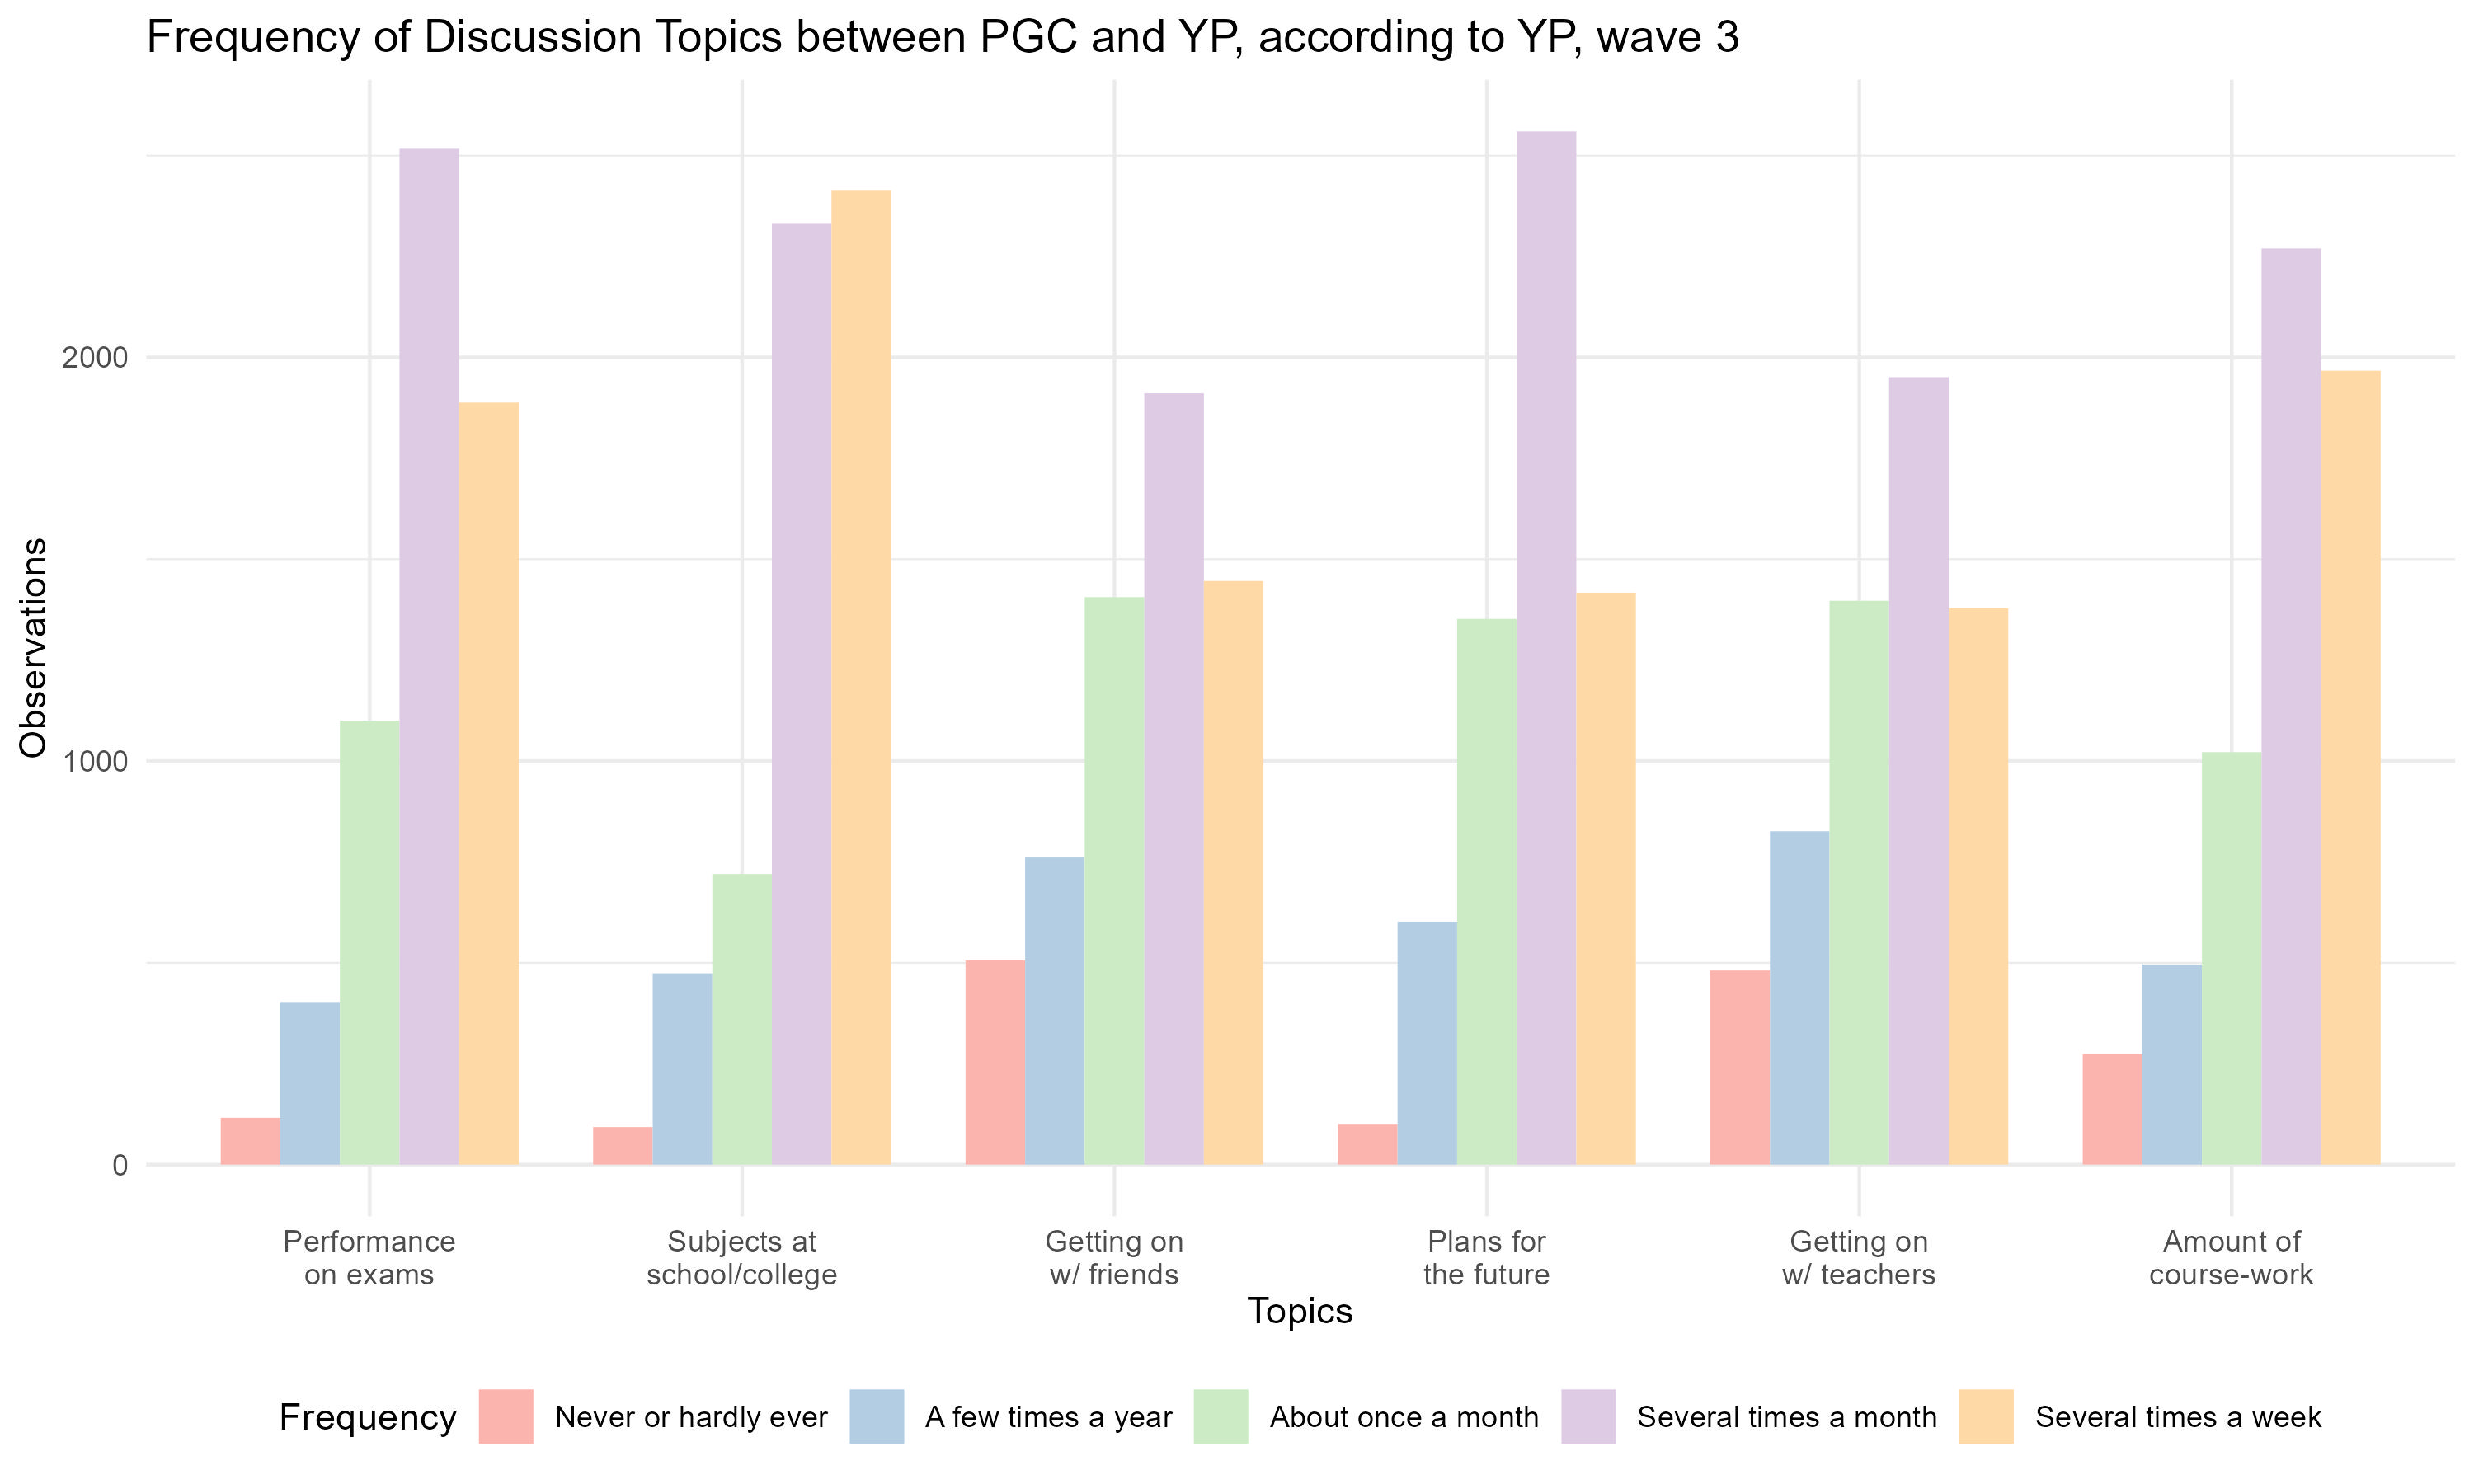
\includegraphics[width=1.15\linewidth]{discussed_topics_plot_YP.jpeg}}
    \caption{Frequency of discussion topics between PCG and YP, according to YP, wave 3}
    \label{}
\end{figure}

\begin{figure}[htbp] 
    \centering
    \rotatebox{90}{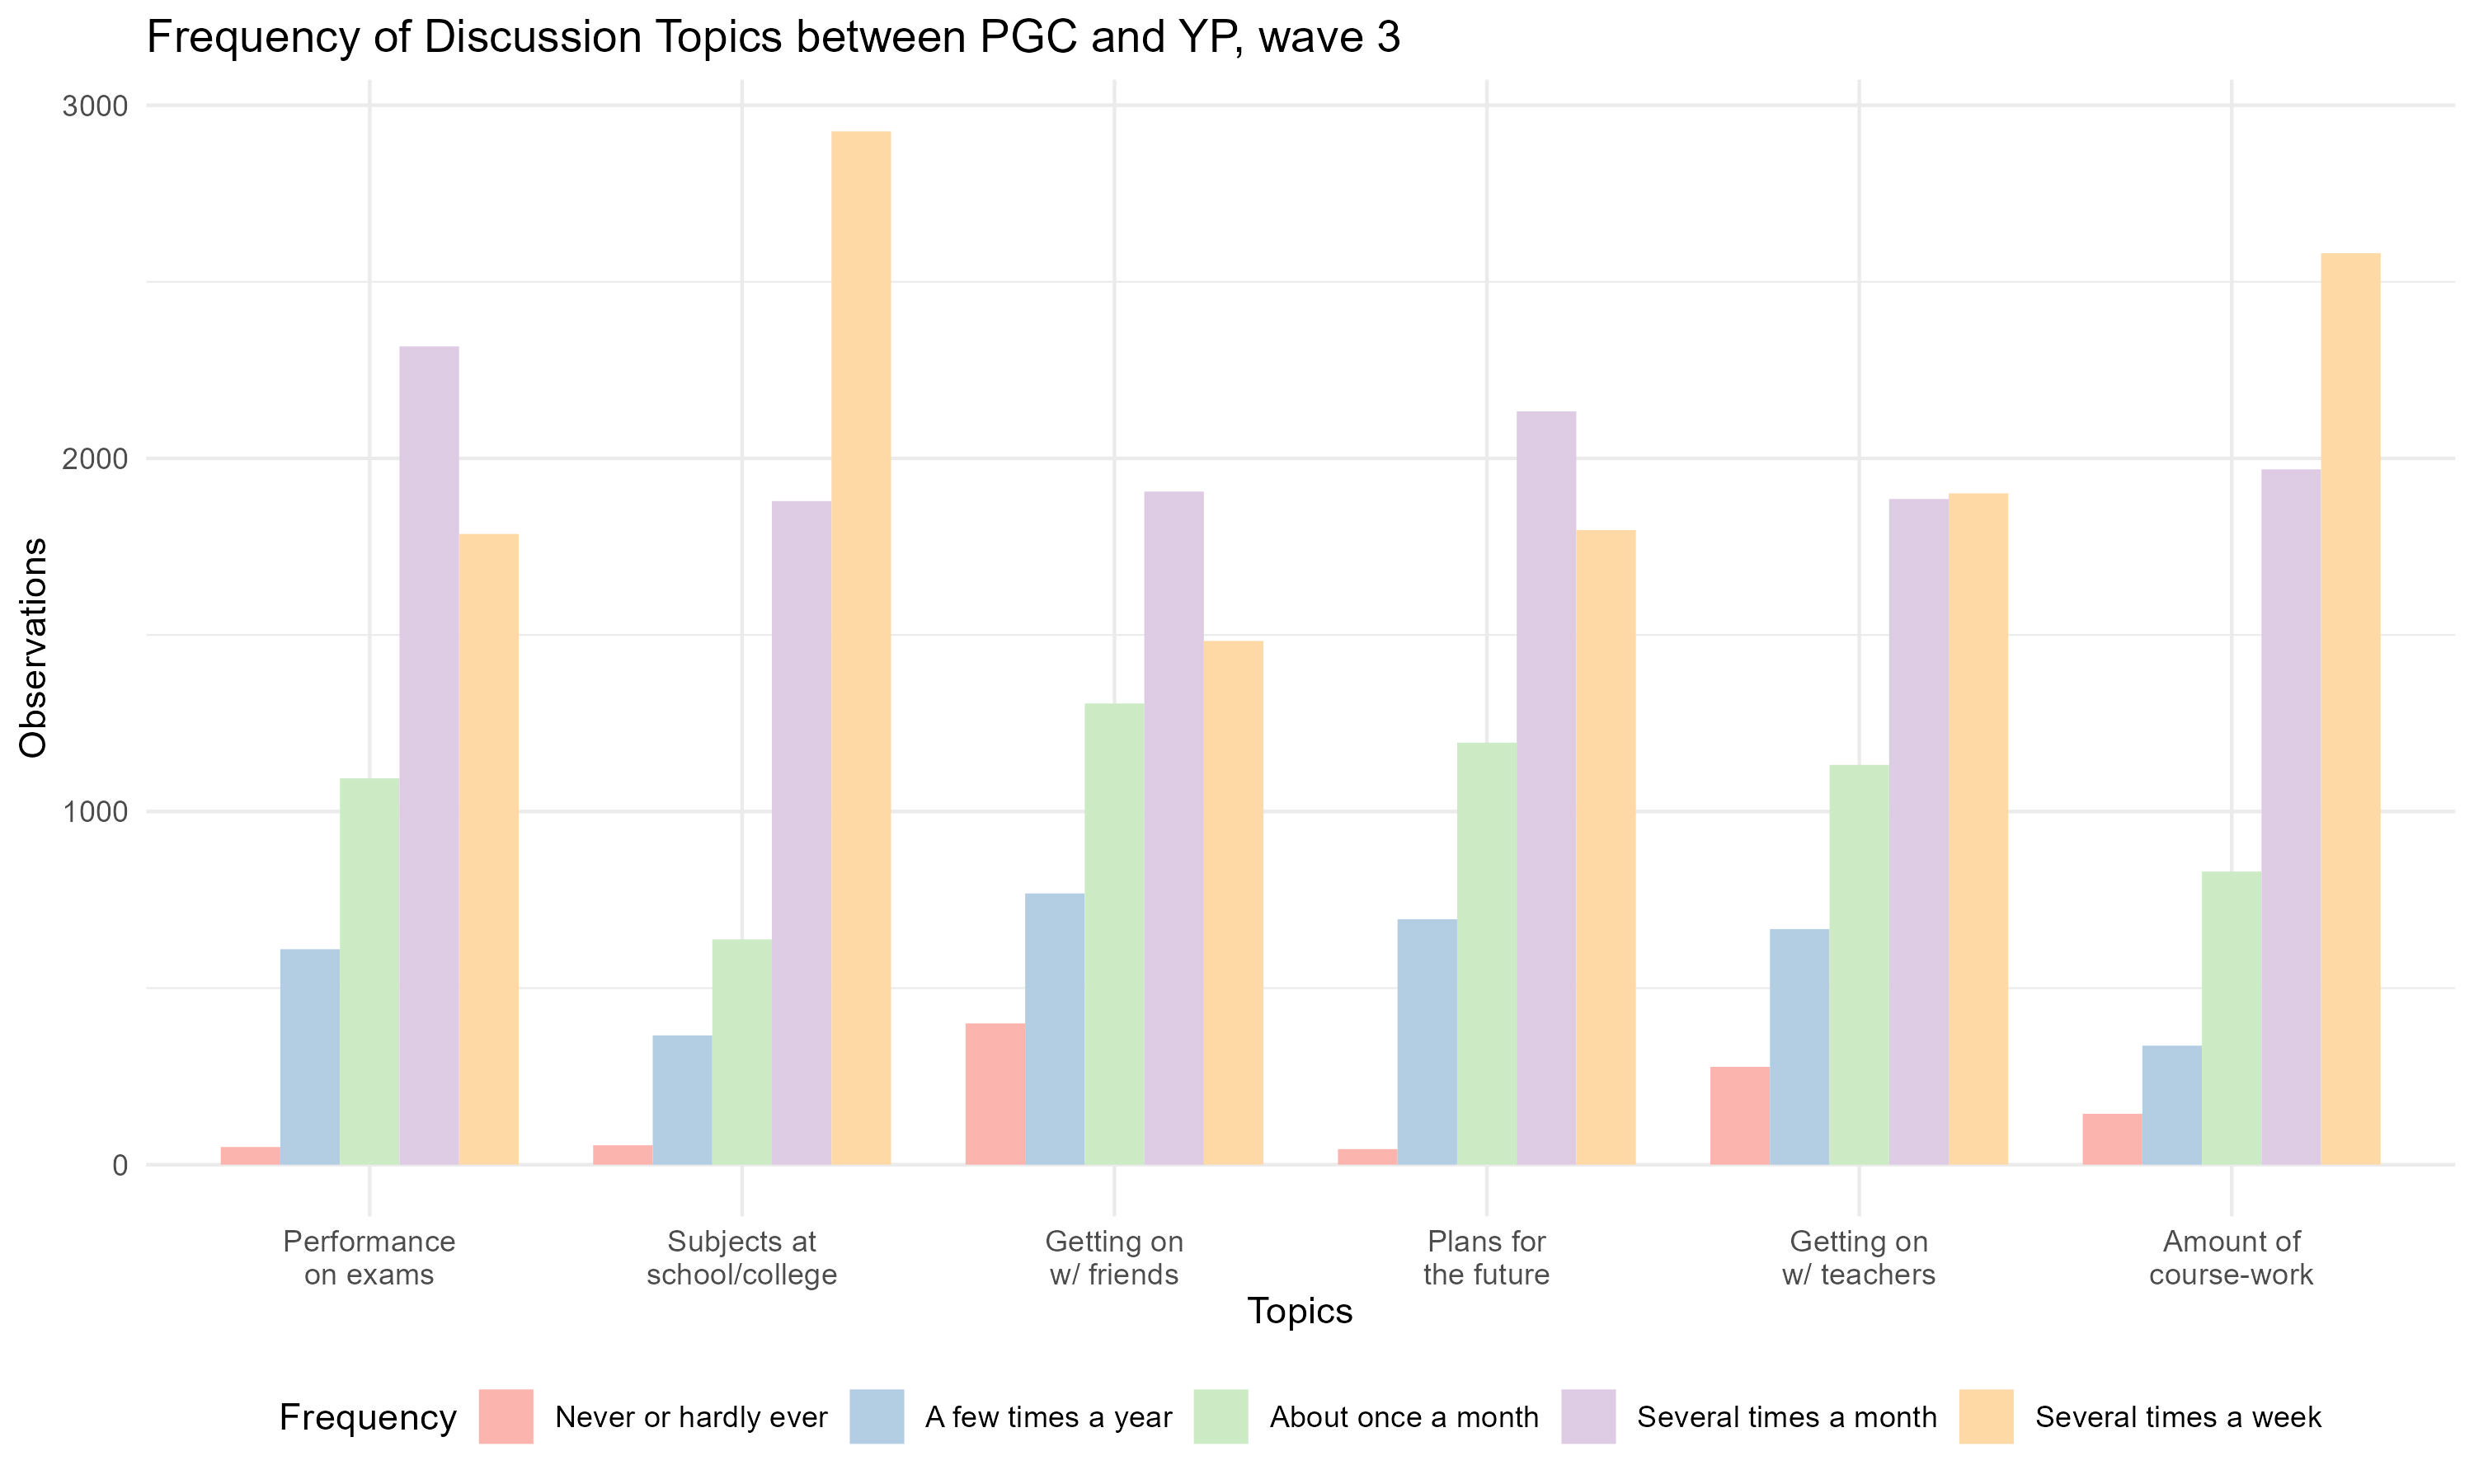
\includegraphics[width=1.15\linewidth]{discussed_topics_plot.jpeg}}
    \caption{Frequency of discussion topics between PCG and YP, according to PCG, wave 3}
    \label{}
\end{figure}

\clearpage
\subsection{TIPI scores}
\begin{figure}[htbp] 
    \centering
    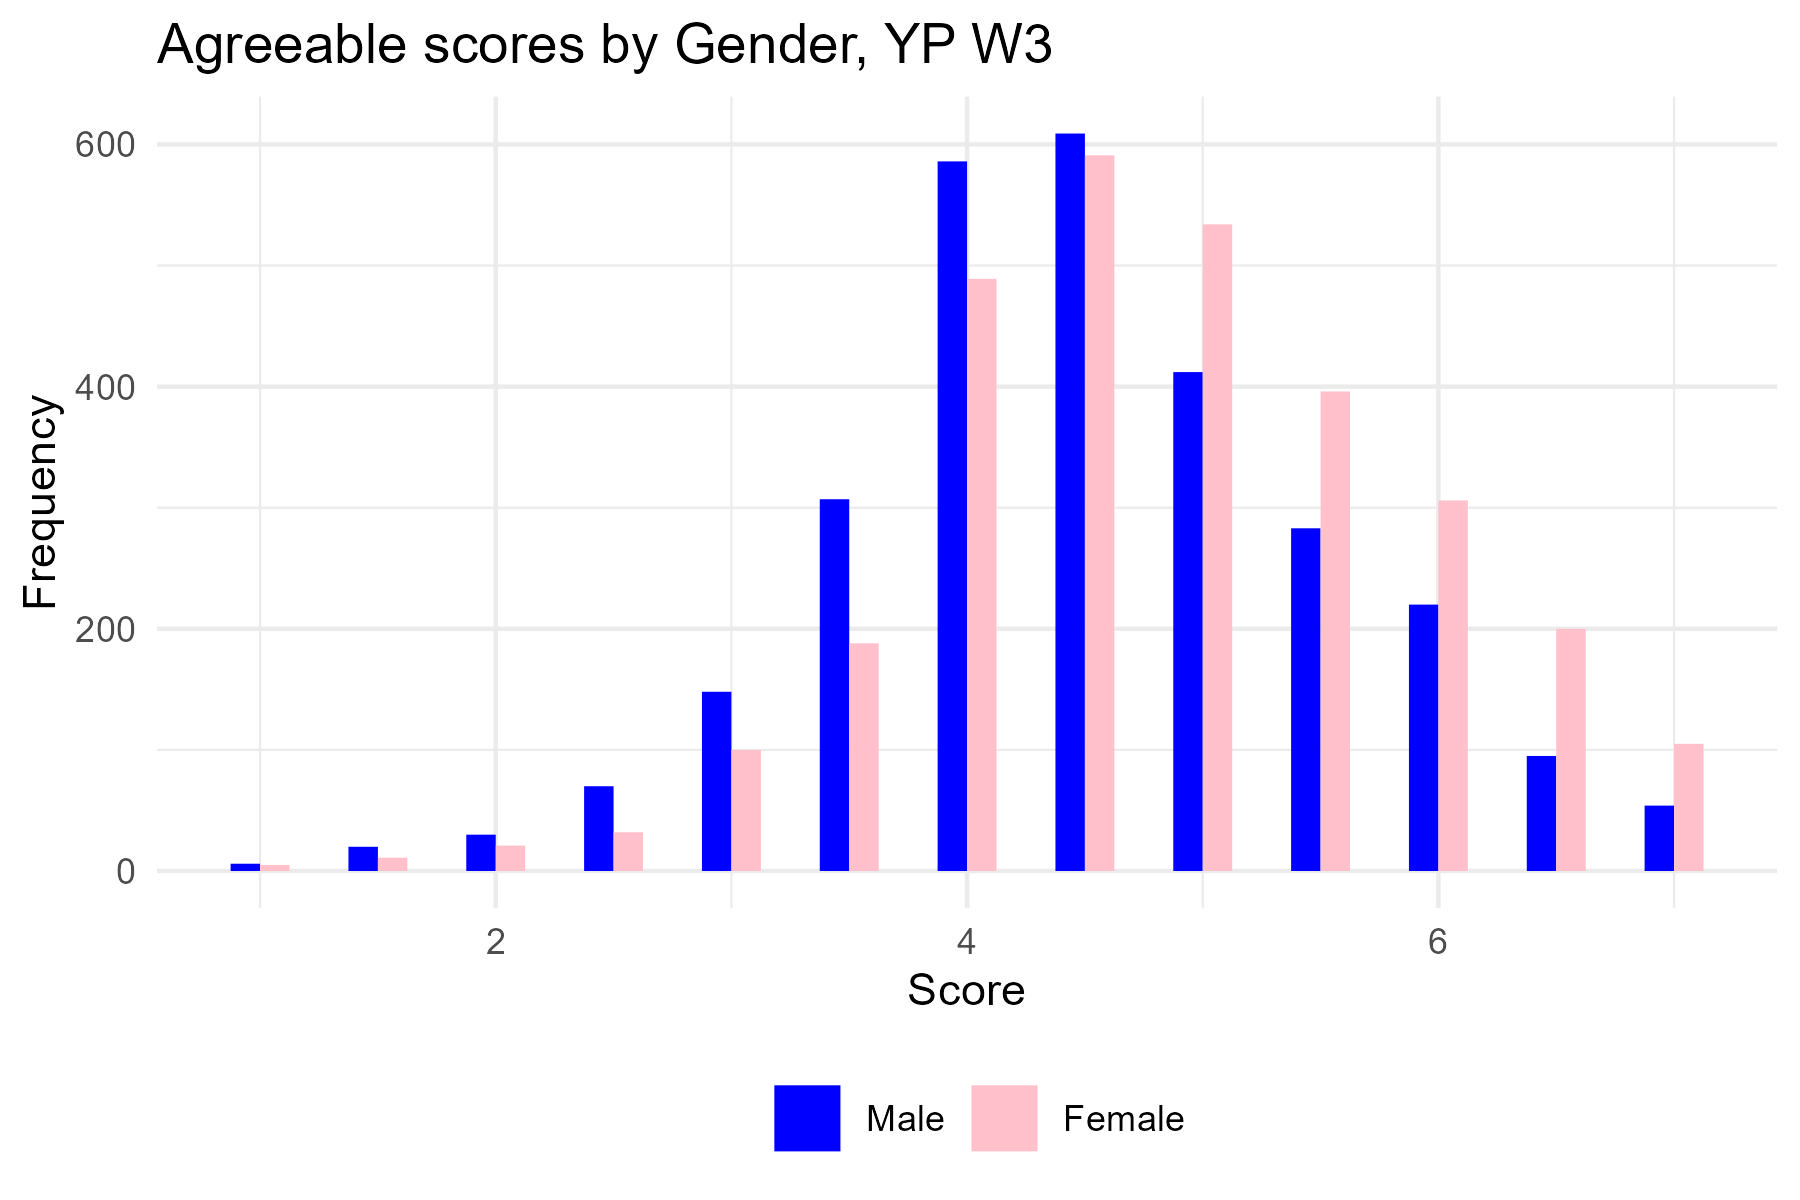
\includegraphics[width=1\linewidth]{Frequency of Agreeable by Gender.jpeg}
    \caption{Frequency of Agreeable scores by gender, reported by YP in wave 3}
    \label{}
\end{figure}

\begin{figure}[htbp] 
    \centering
    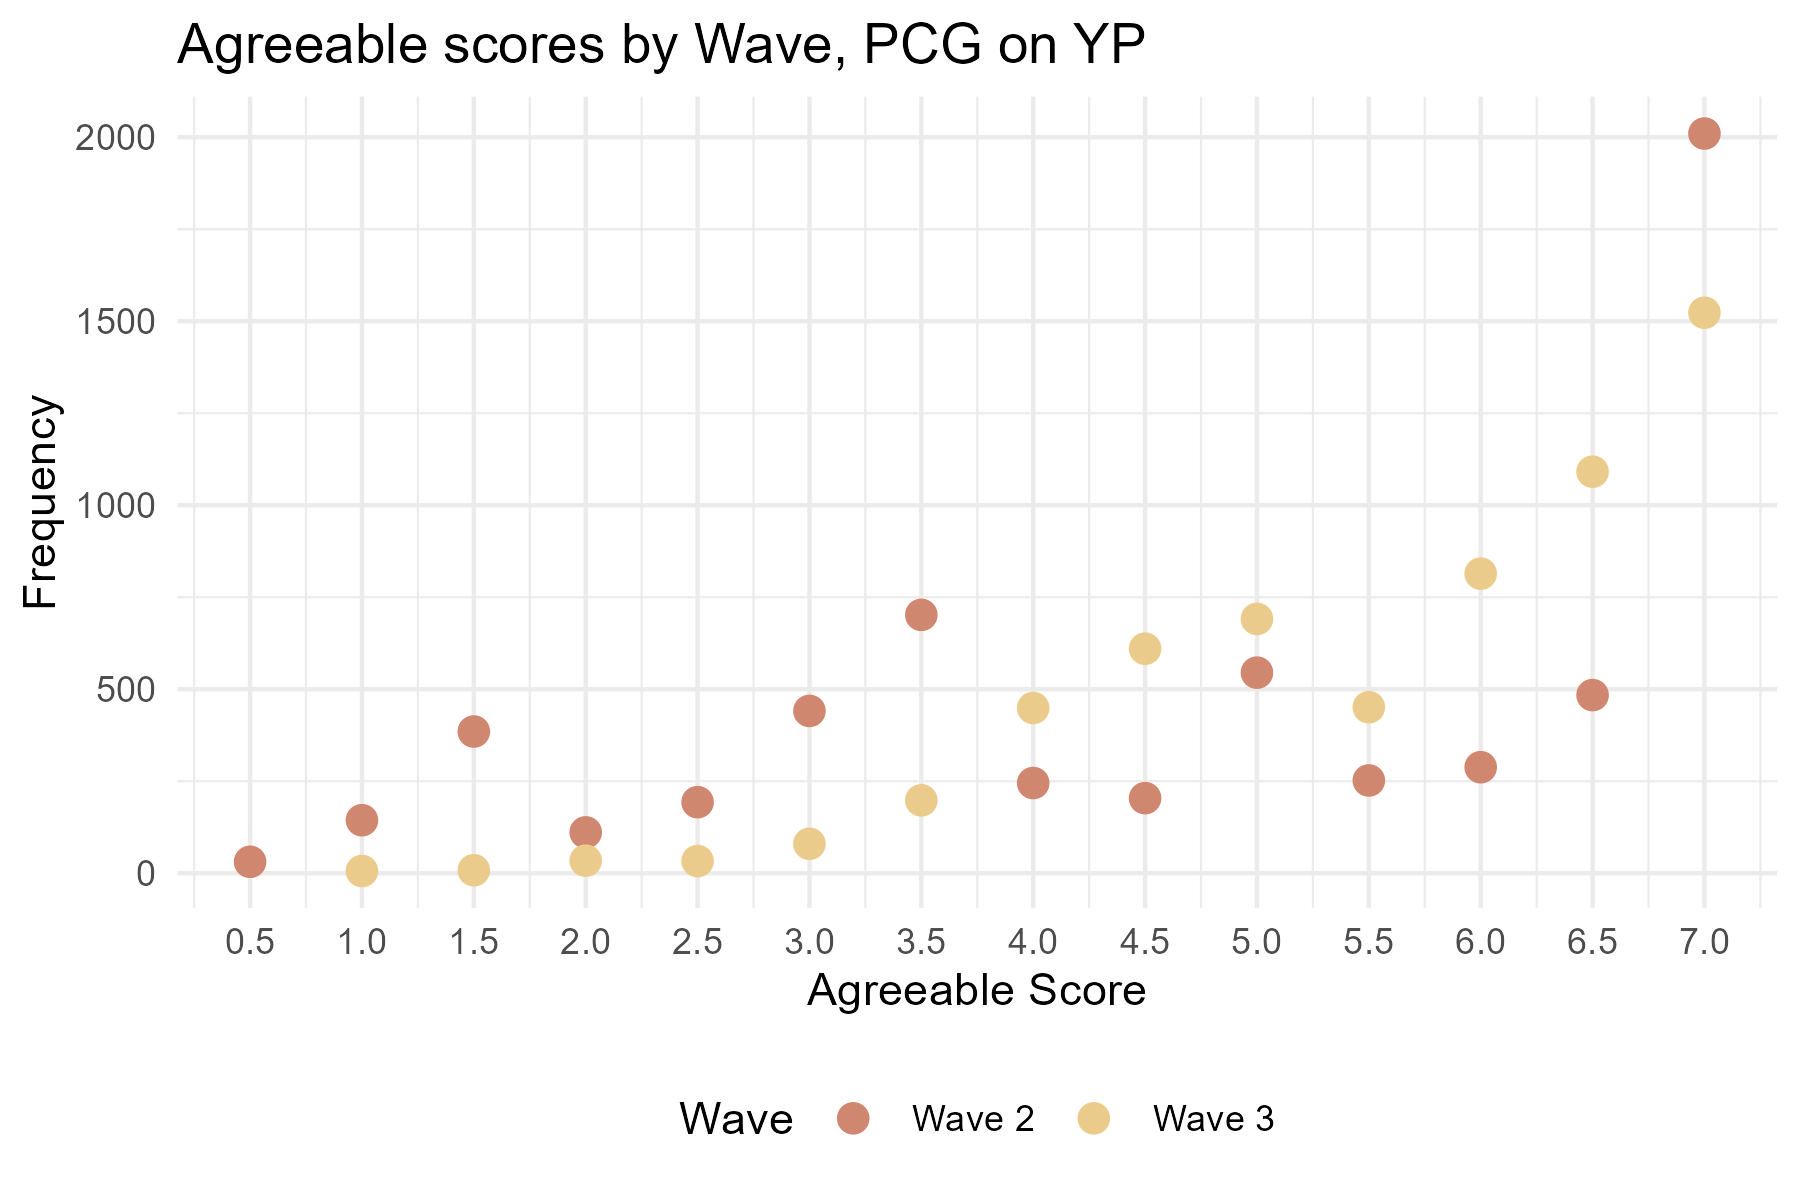
\includegraphics[width=1\linewidth]{Frequency of Agreeable by Wave, PCG.jpeg}
    \caption{Frequency of YP's Agreeable scores reported by PCG in waves 2 and 3}
    \label{}
\end{figure}

\begin{figure}[htbp] 
    \centering
    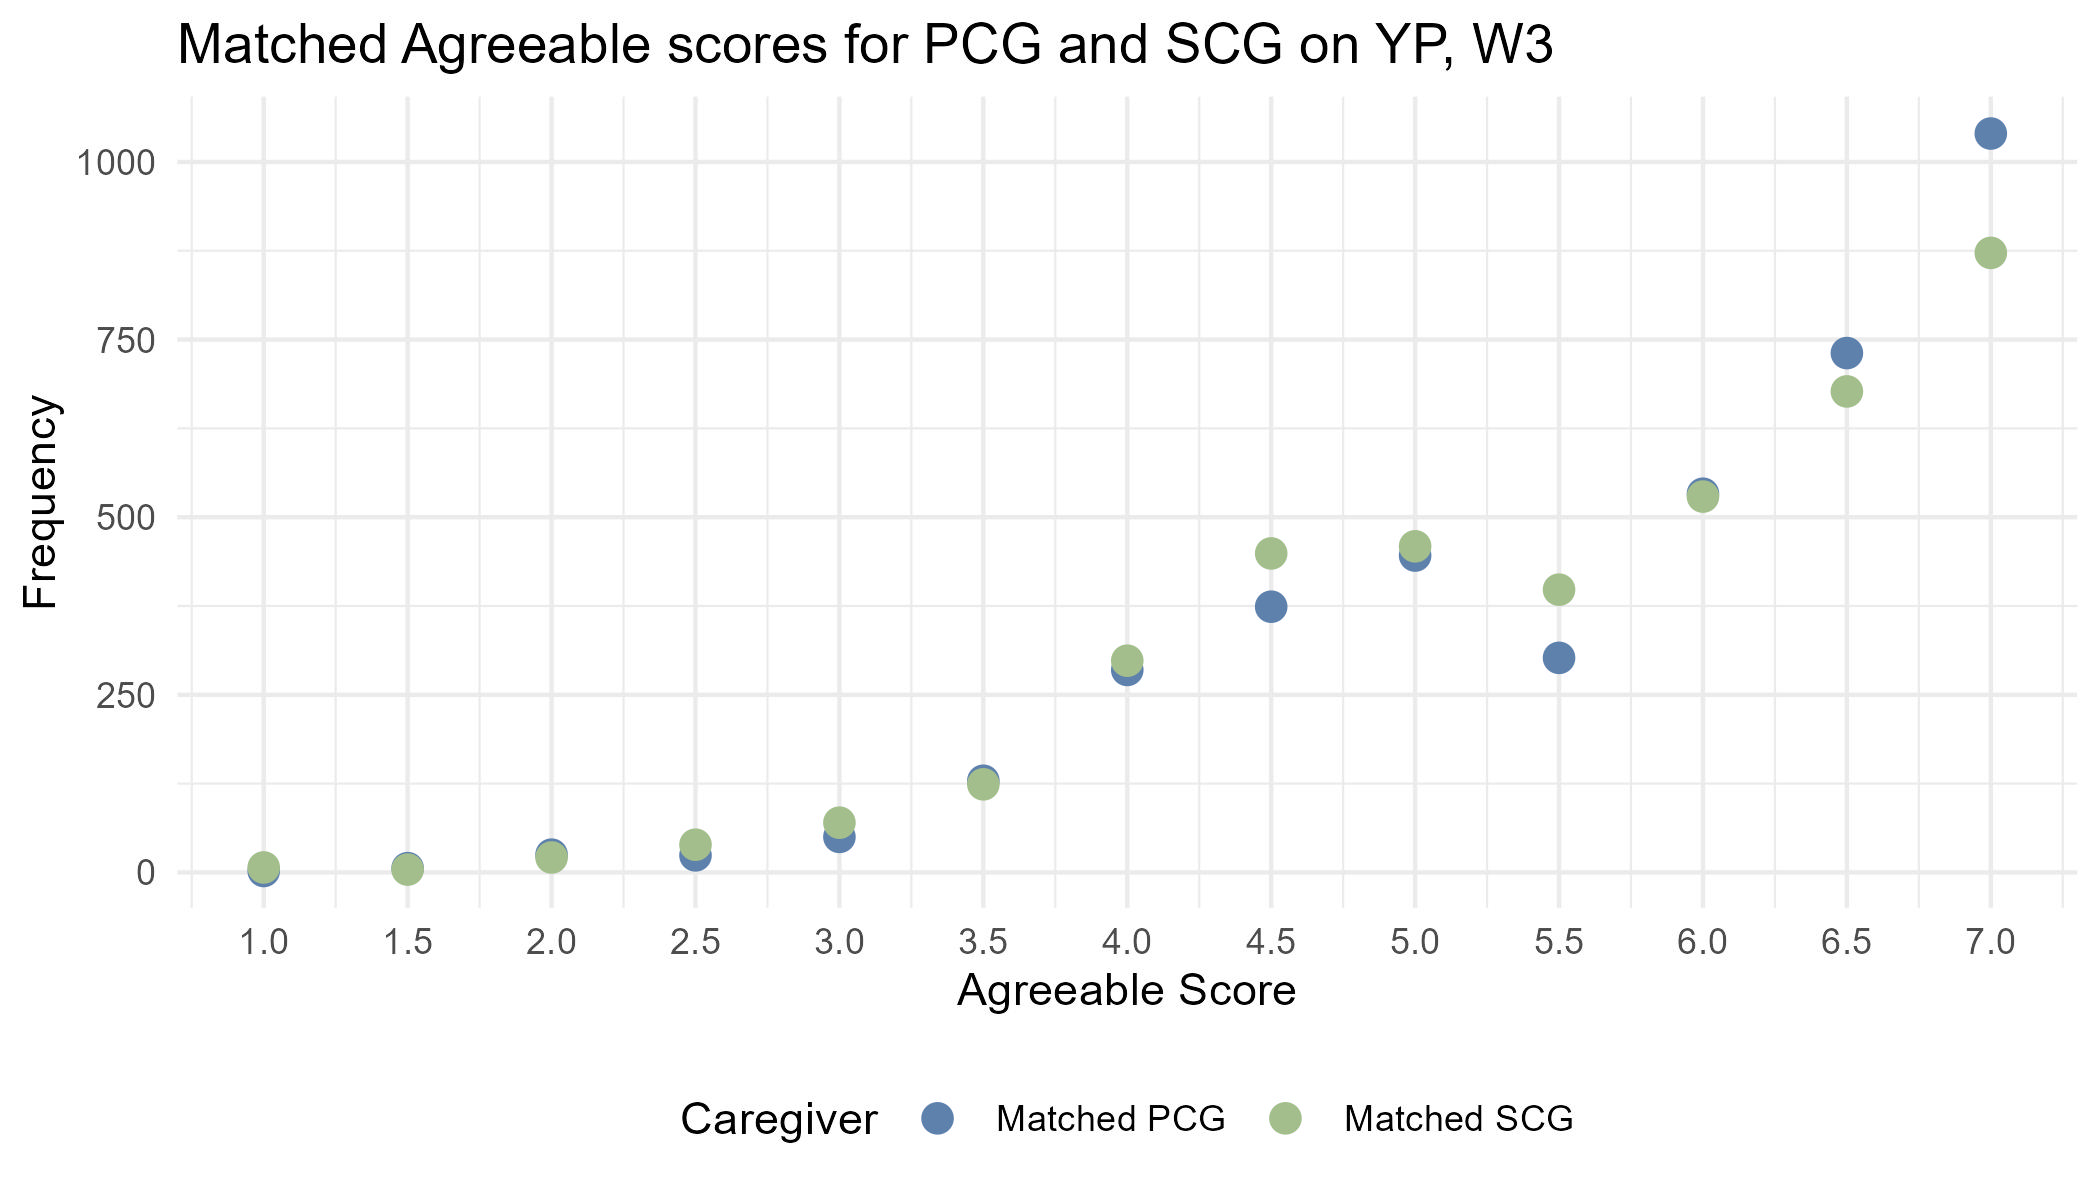
\includegraphics[width=1\linewidth]{Matched Agreeable by participant w3.jpeg}
    \caption{Frequency of YP's Agreeable scores reported by PCG and SCG in wave 3 (matched)}
    \label{}
\end{figure}

\begin{figure}[htbp] 
    \centering
    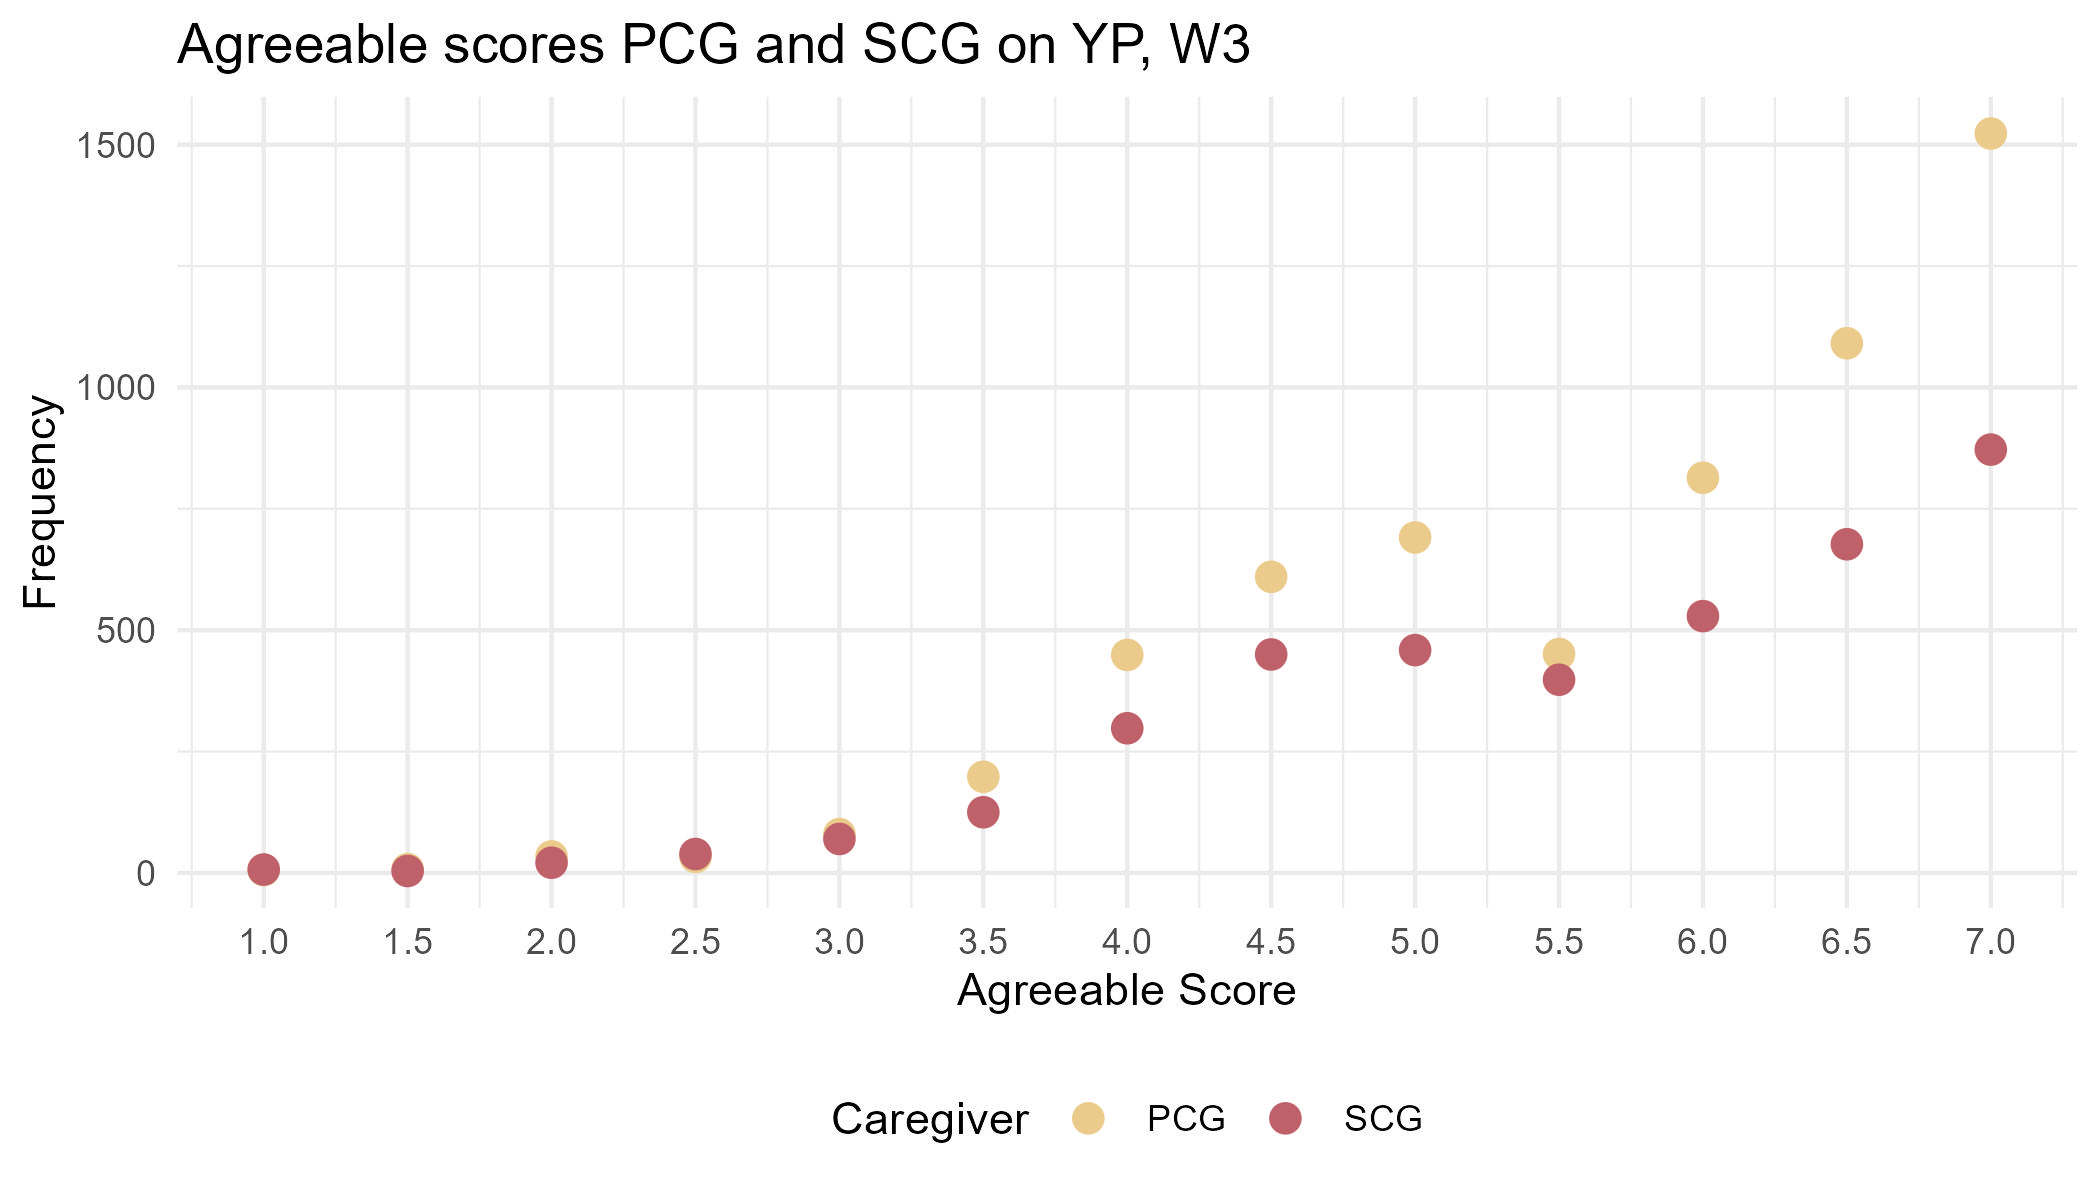
\includegraphics[width=1\linewidth]{Frequency of Agreeable by participant w3.jpeg}
    \caption{Frequency of YP's Agreeable scores reported by PCG and SCG in wave 3 (not matched)}
    \label{}
\end{figure}

\begin{figure}[htbp] 
    \centering
    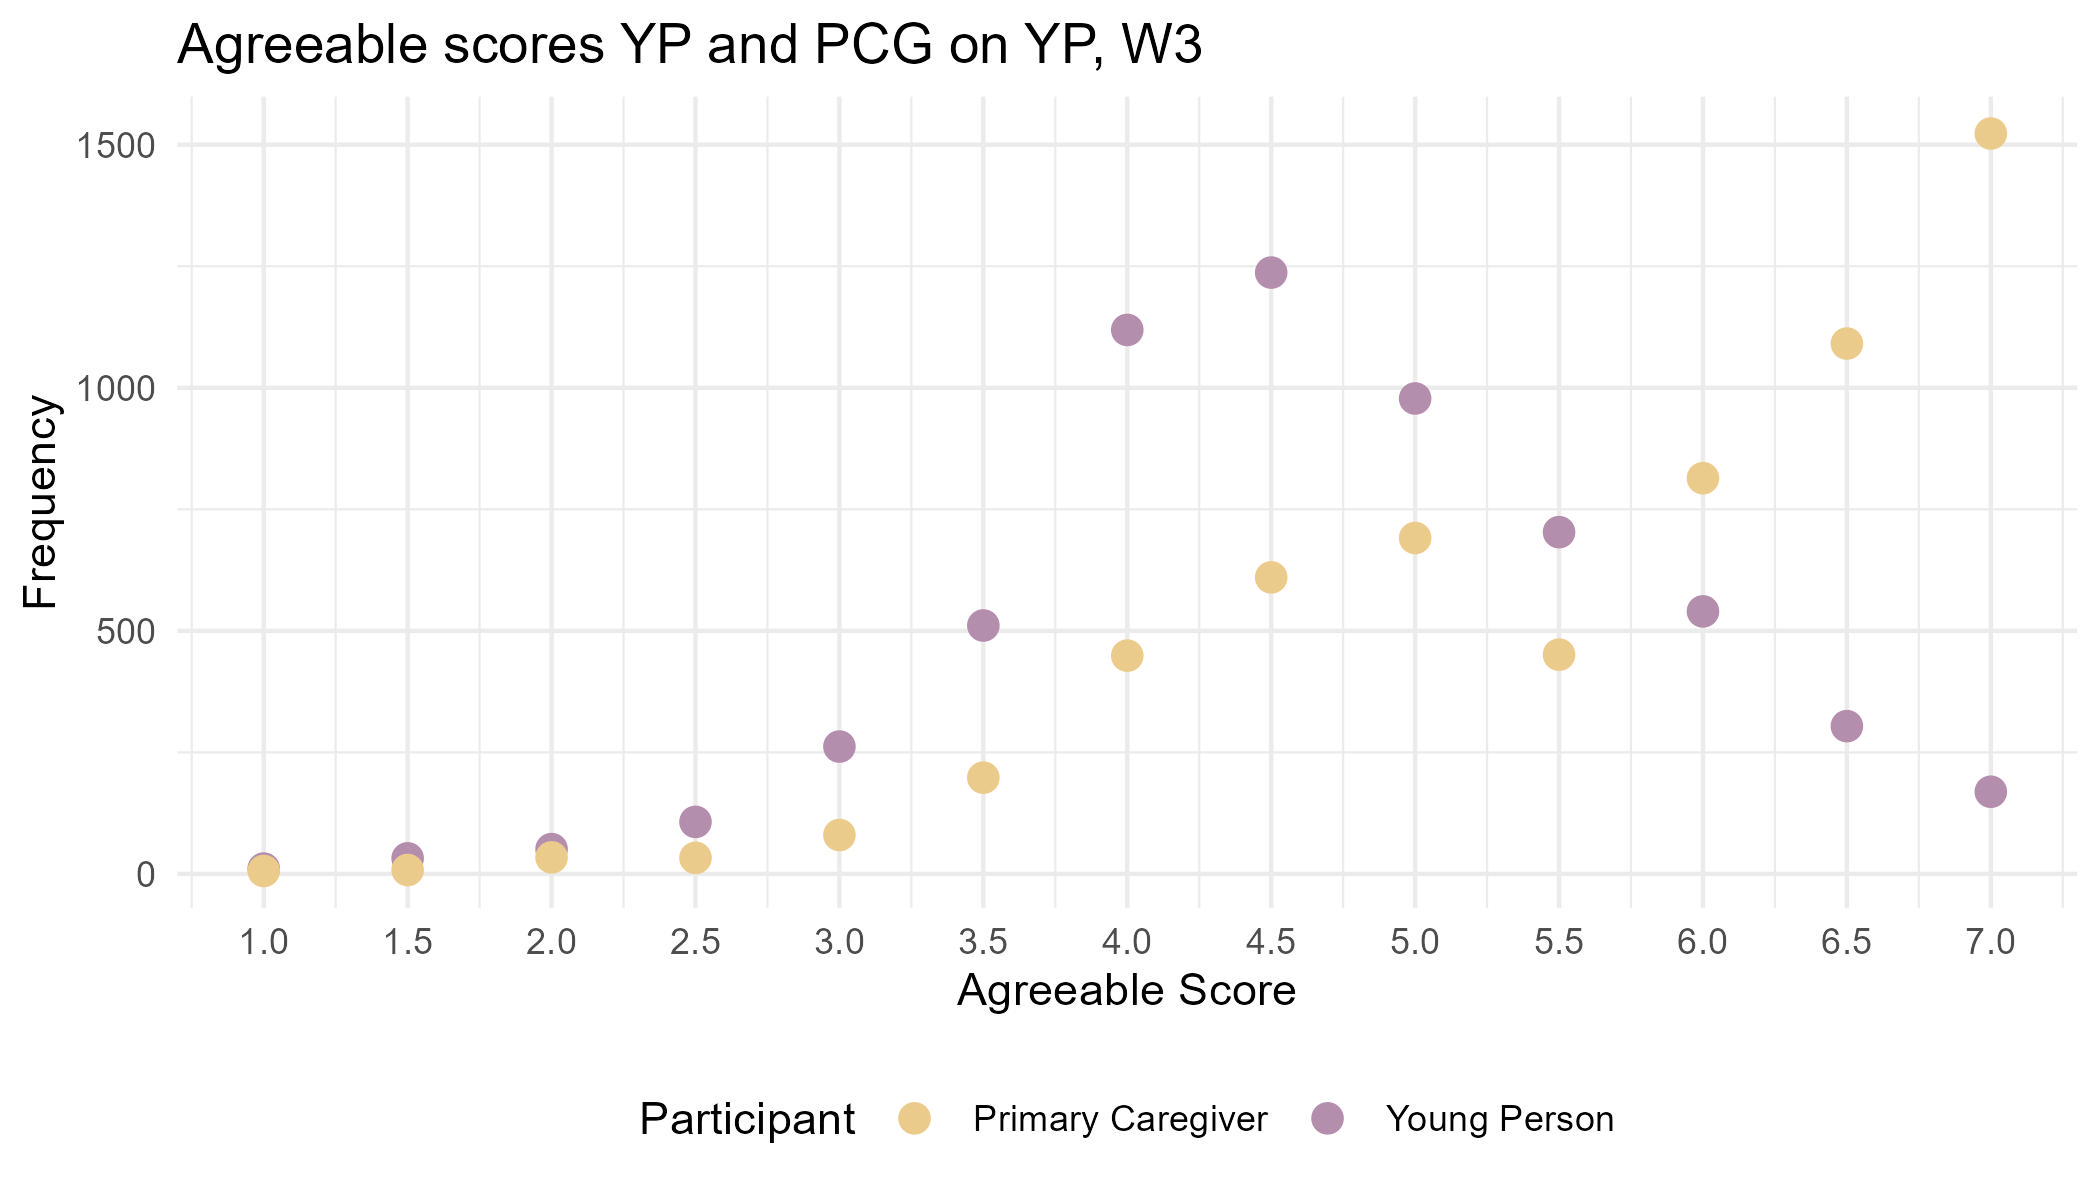
\includegraphics[width=1\linewidth]{Frequency of Agreeable by participant w3a.jpeg}
    \caption{Frequency of YP's Agreeable scores reported by YP and PCG in wave 3}
    \label{}
\end{figure}


\begin{figure}[htbp] 
    \centering
    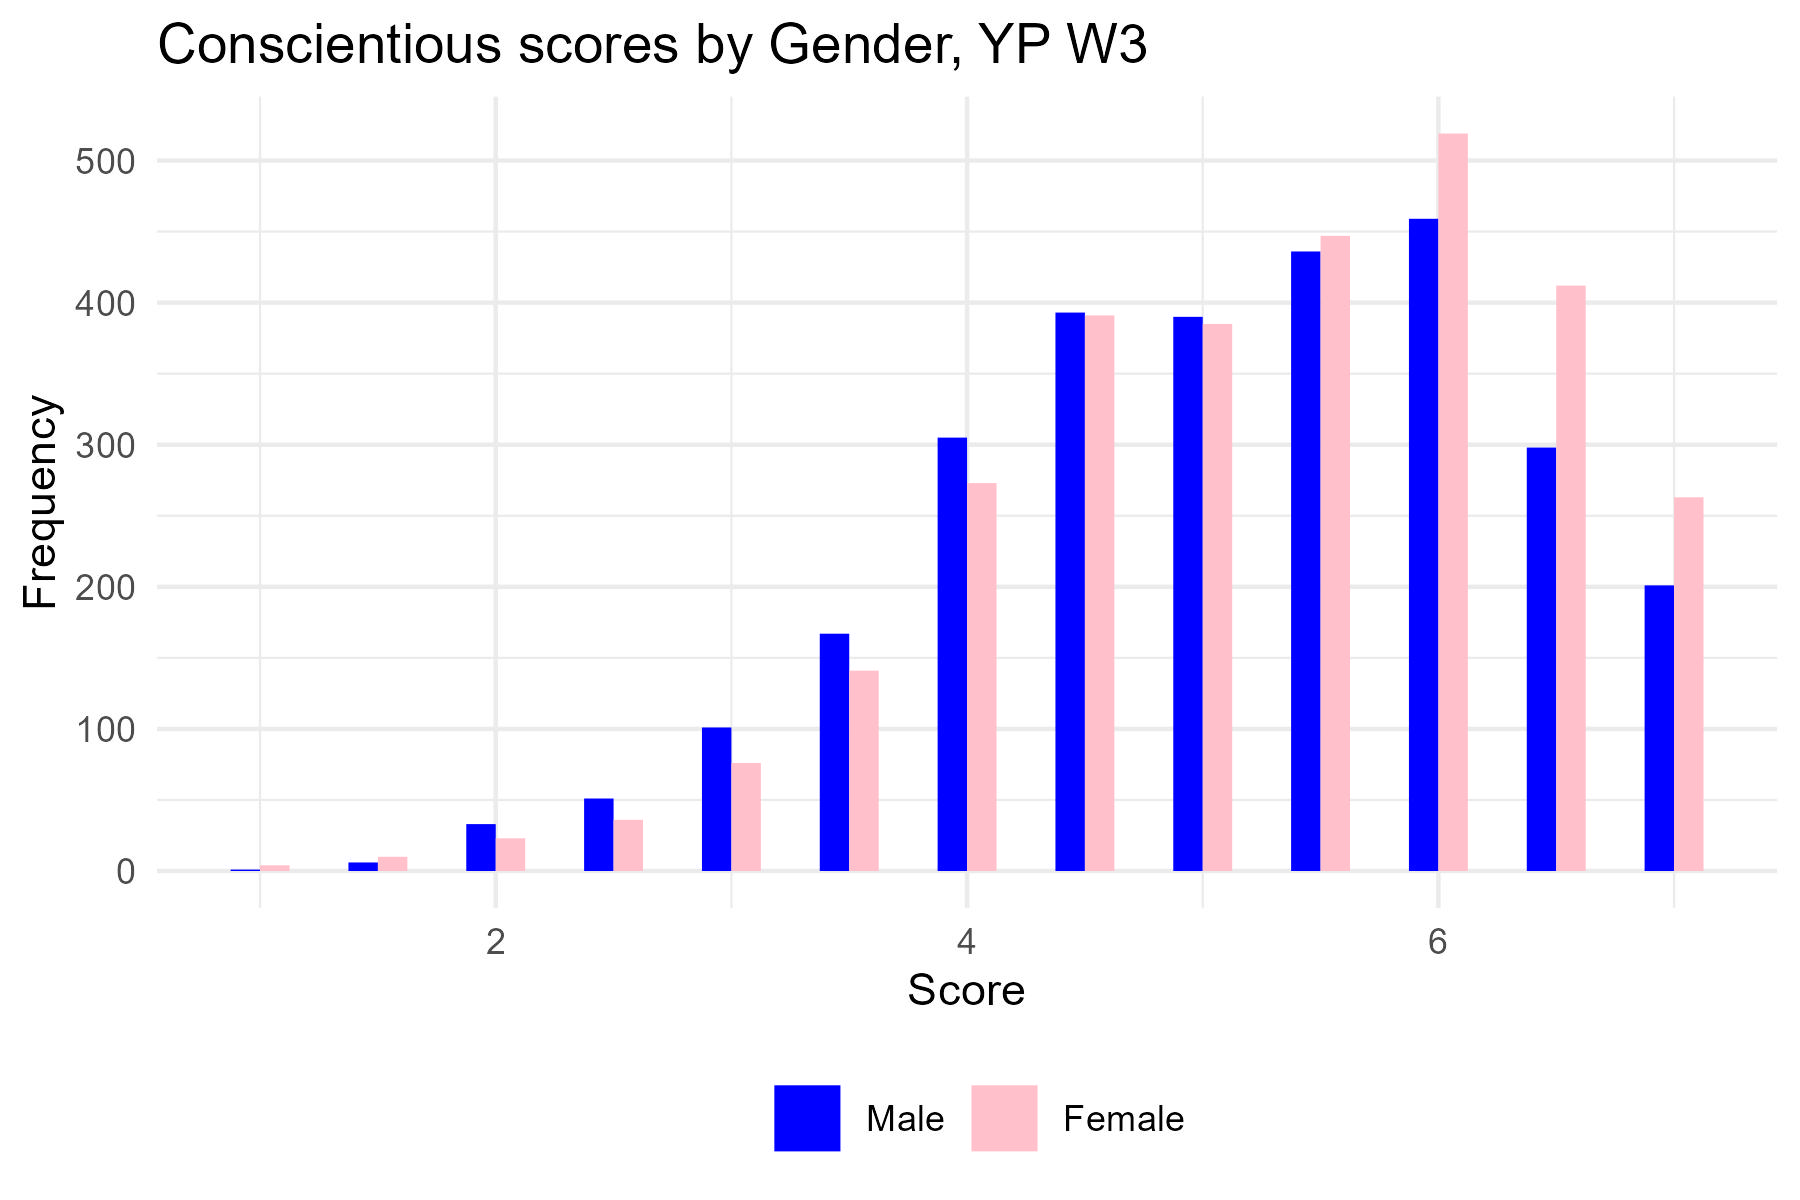
\includegraphics[width=1\linewidth]{Frequency of Conscientious by Gender.jpeg}
    \caption{Frequency of Conscientious scores by gender, reported by YP in wave 3}
    \label{}
\end{figure}

\begin{figure}[htbp] 
    \centering
    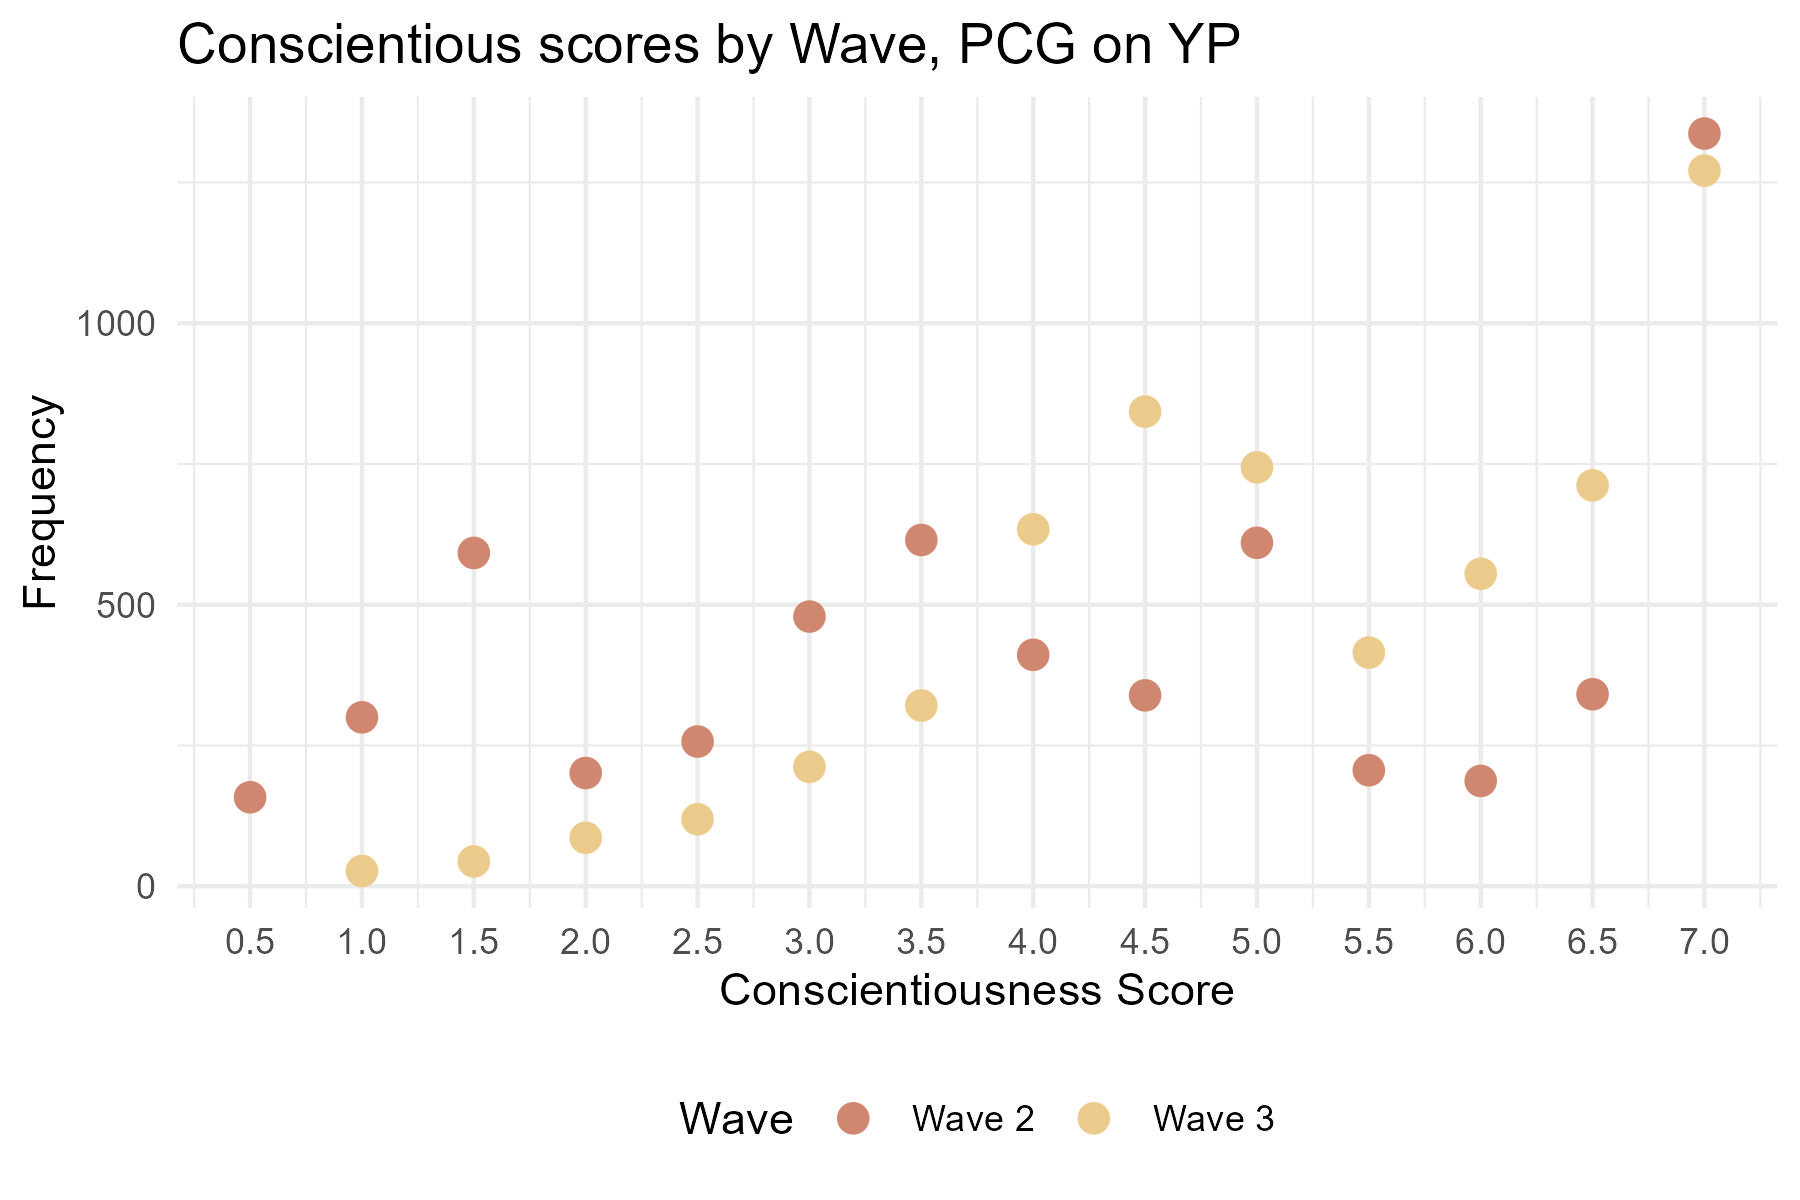
\includegraphics[width=1\linewidth]{Frequency of Conscientious by Wave, PCG.jpeg}
    \caption{Frequency of YP's Conscientious scores reported by PCG in waves 2 and 3}
    \label{}
\end{figure}

\begin{figure}[htbp] 
    \centering
    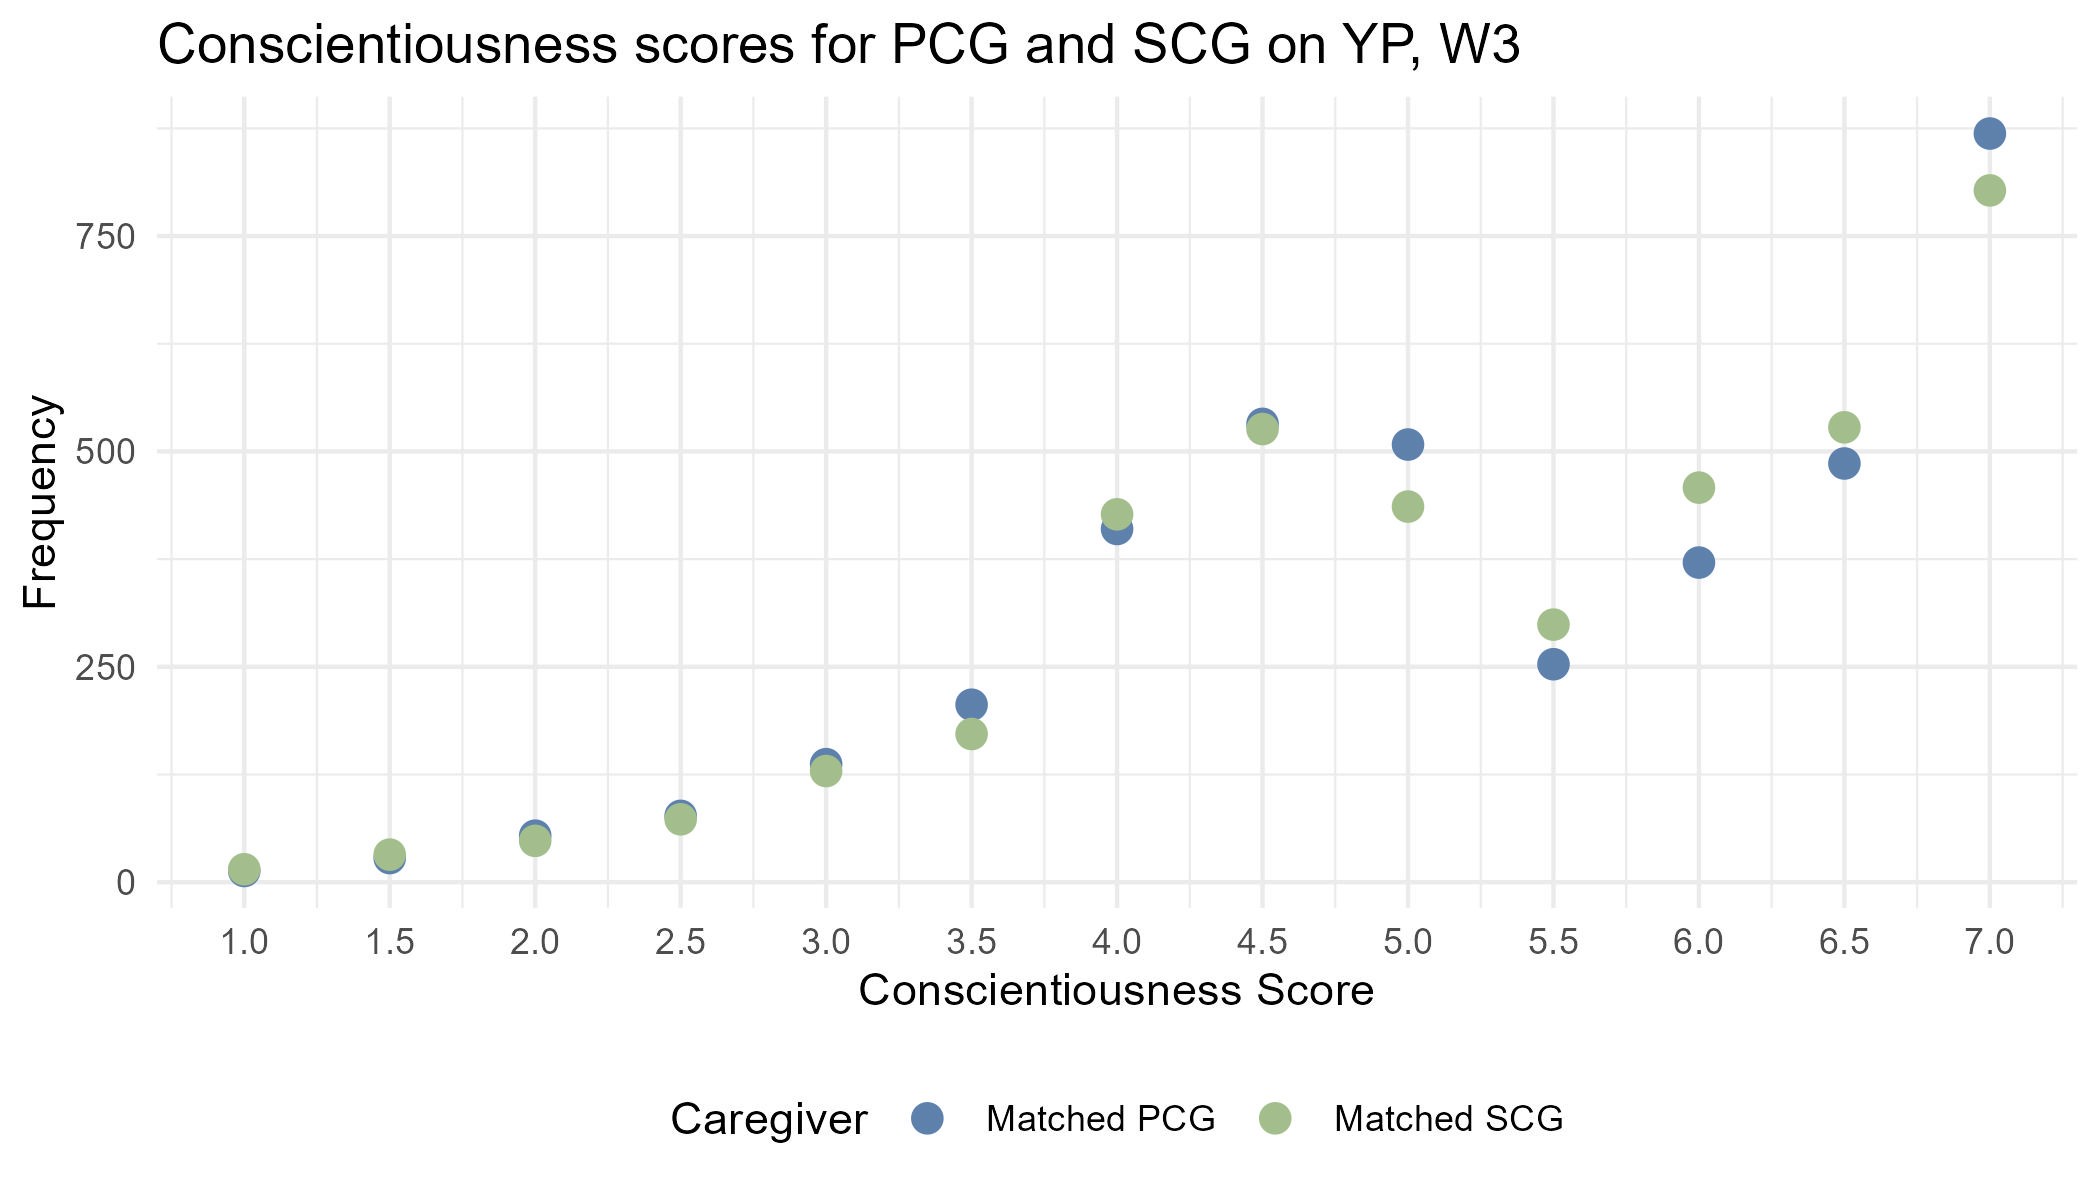
\includegraphics[width=1\linewidth]{Matched Conscientious by participant w3.jpeg}
    \caption{Frequency of YP's Conscientious scores reported by PCG and SCG in wave 3 (matched)}
    \label{}
\end{figure}

\begin{figure}[htbp] 
    \centering
    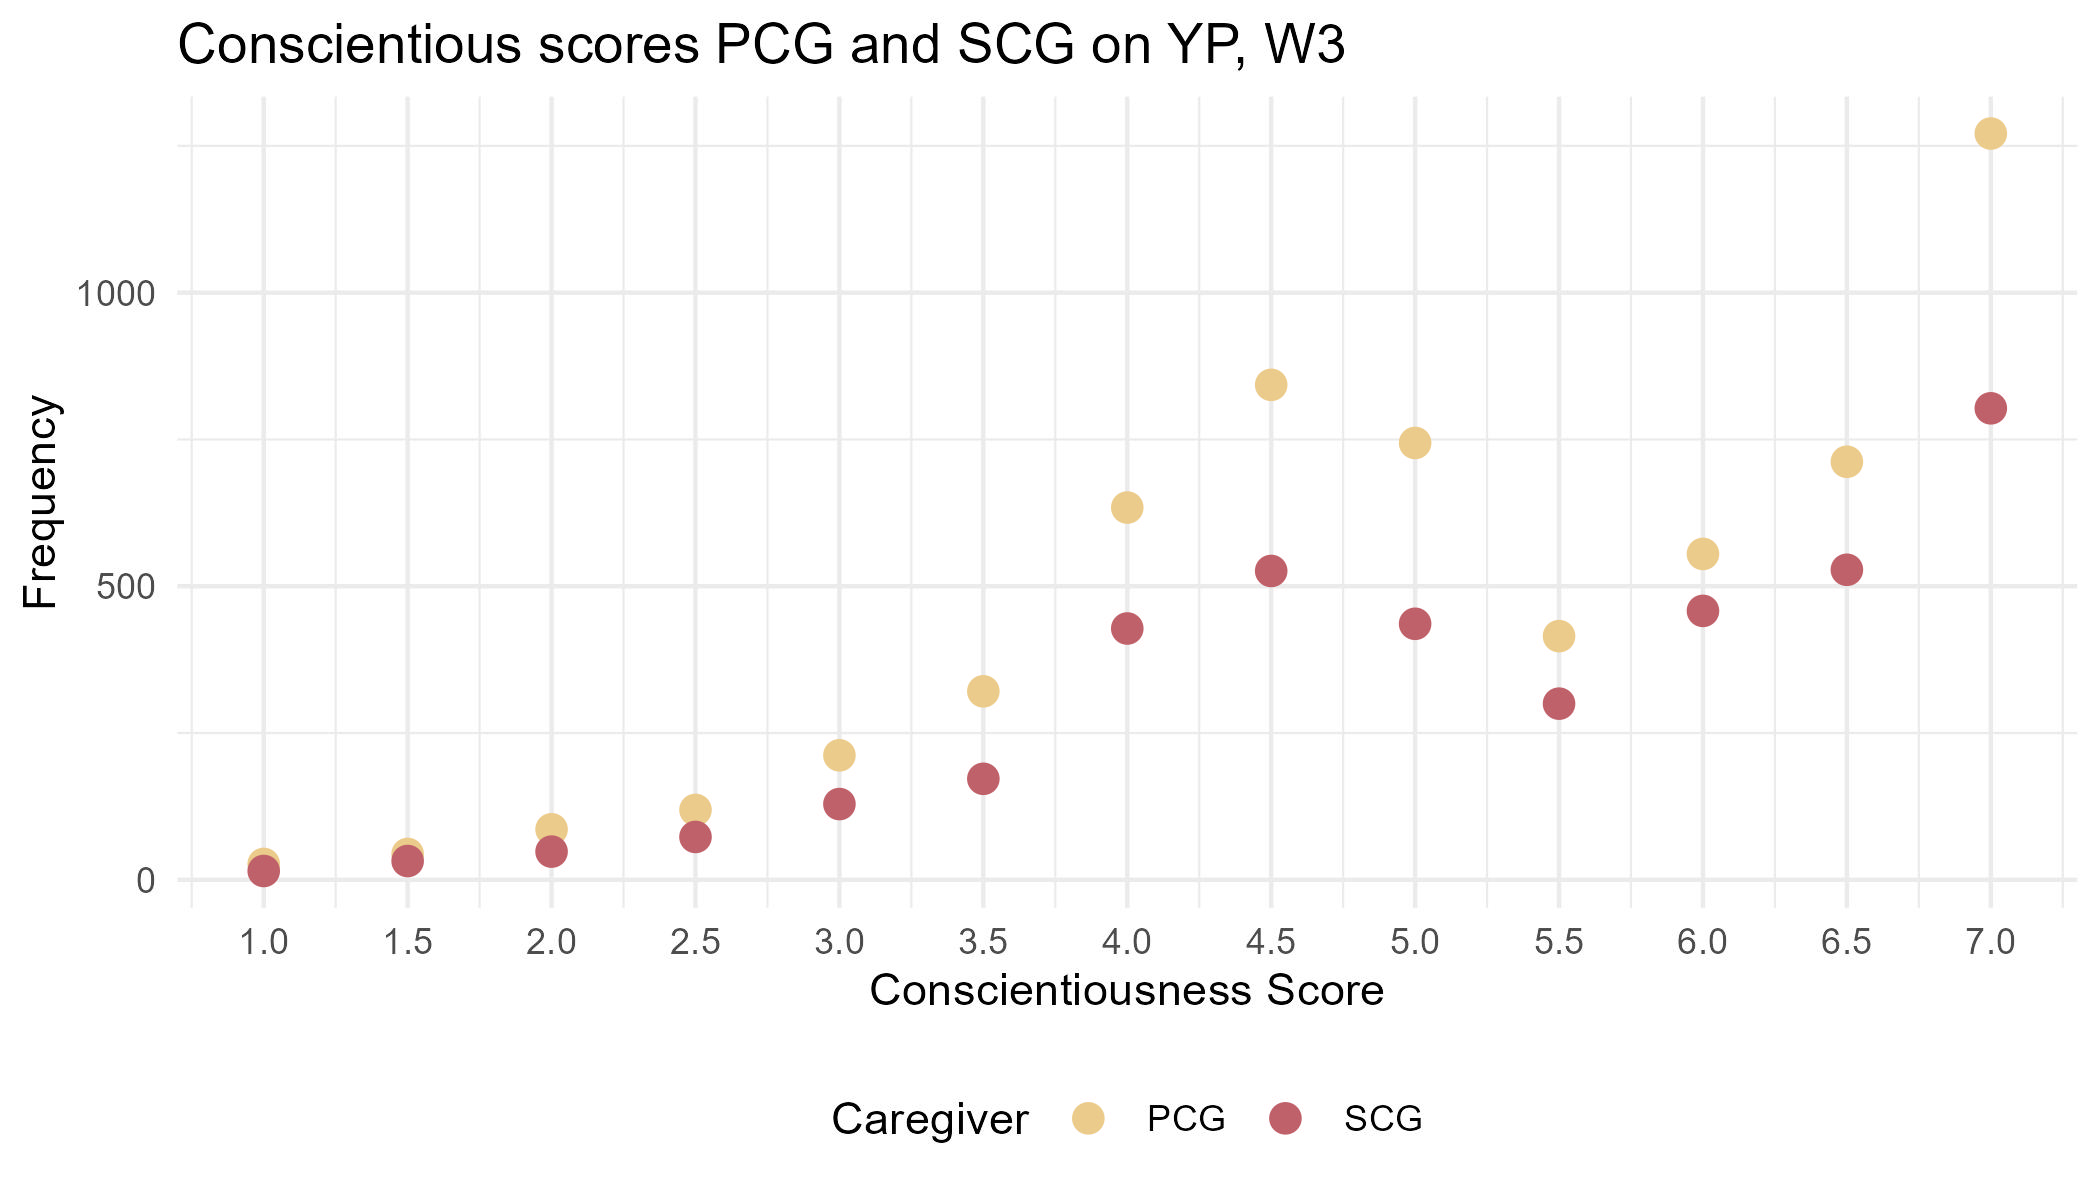
\includegraphics[width=1\linewidth]{Frequency of Conscientious by participant w3.jpeg}
    \caption{Frequency of YP's Conscientious scores reported by PCG and SCG in wave 3 (not matched)}
    \label{}
\end{figure}

\begin{figure}[htbp] 
    \centering
    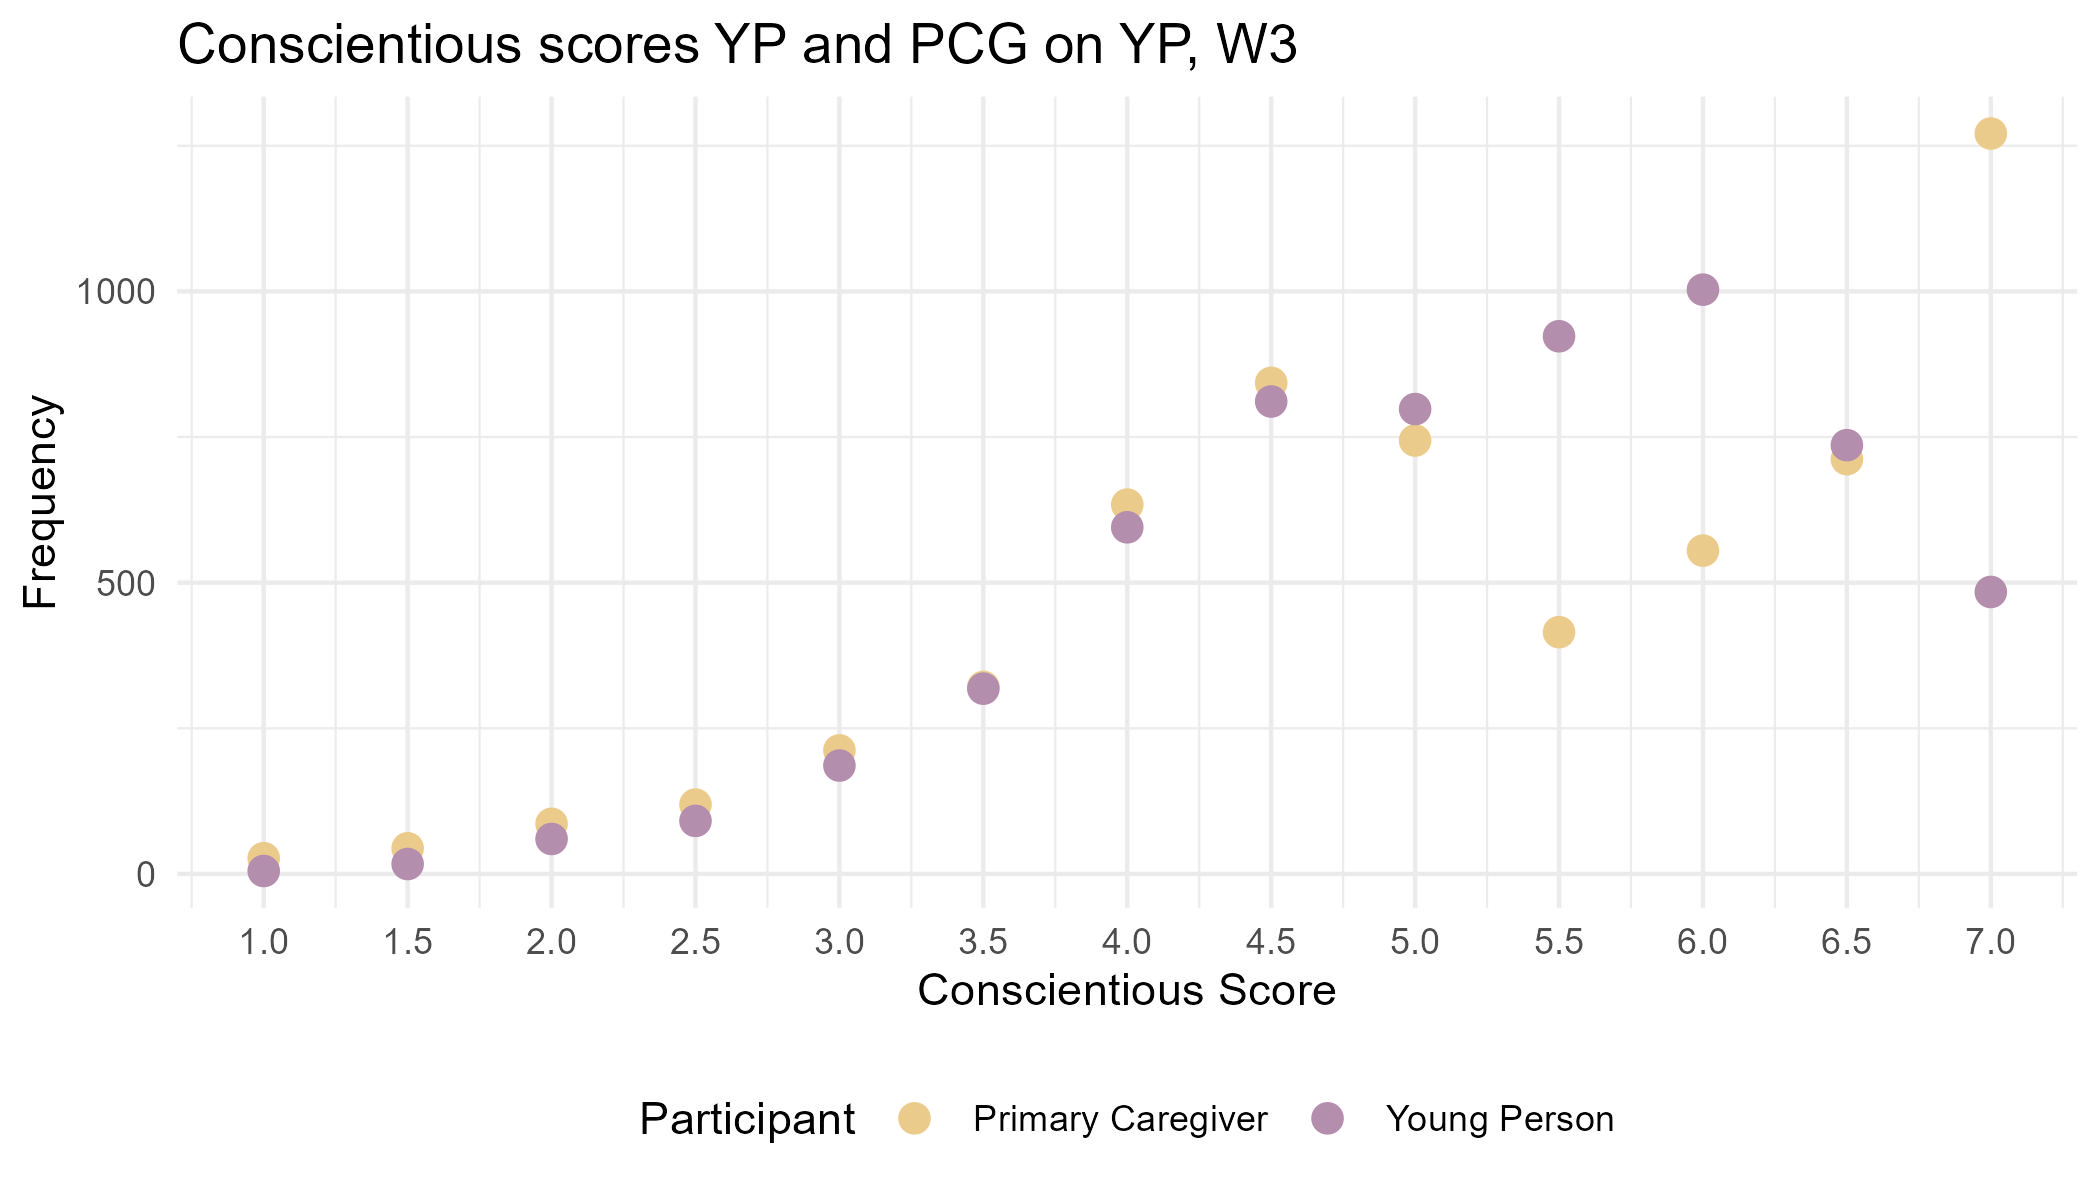
\includegraphics[width=1\linewidth]{Frequency of Conscientious by participant w3a.jpeg}
    \caption{Frequency of YP's Conscientious scores reported by YP and PCG in wave 3}
    \label{}
\end{figure}

\begin{figure}[htbp] 
    \centering
    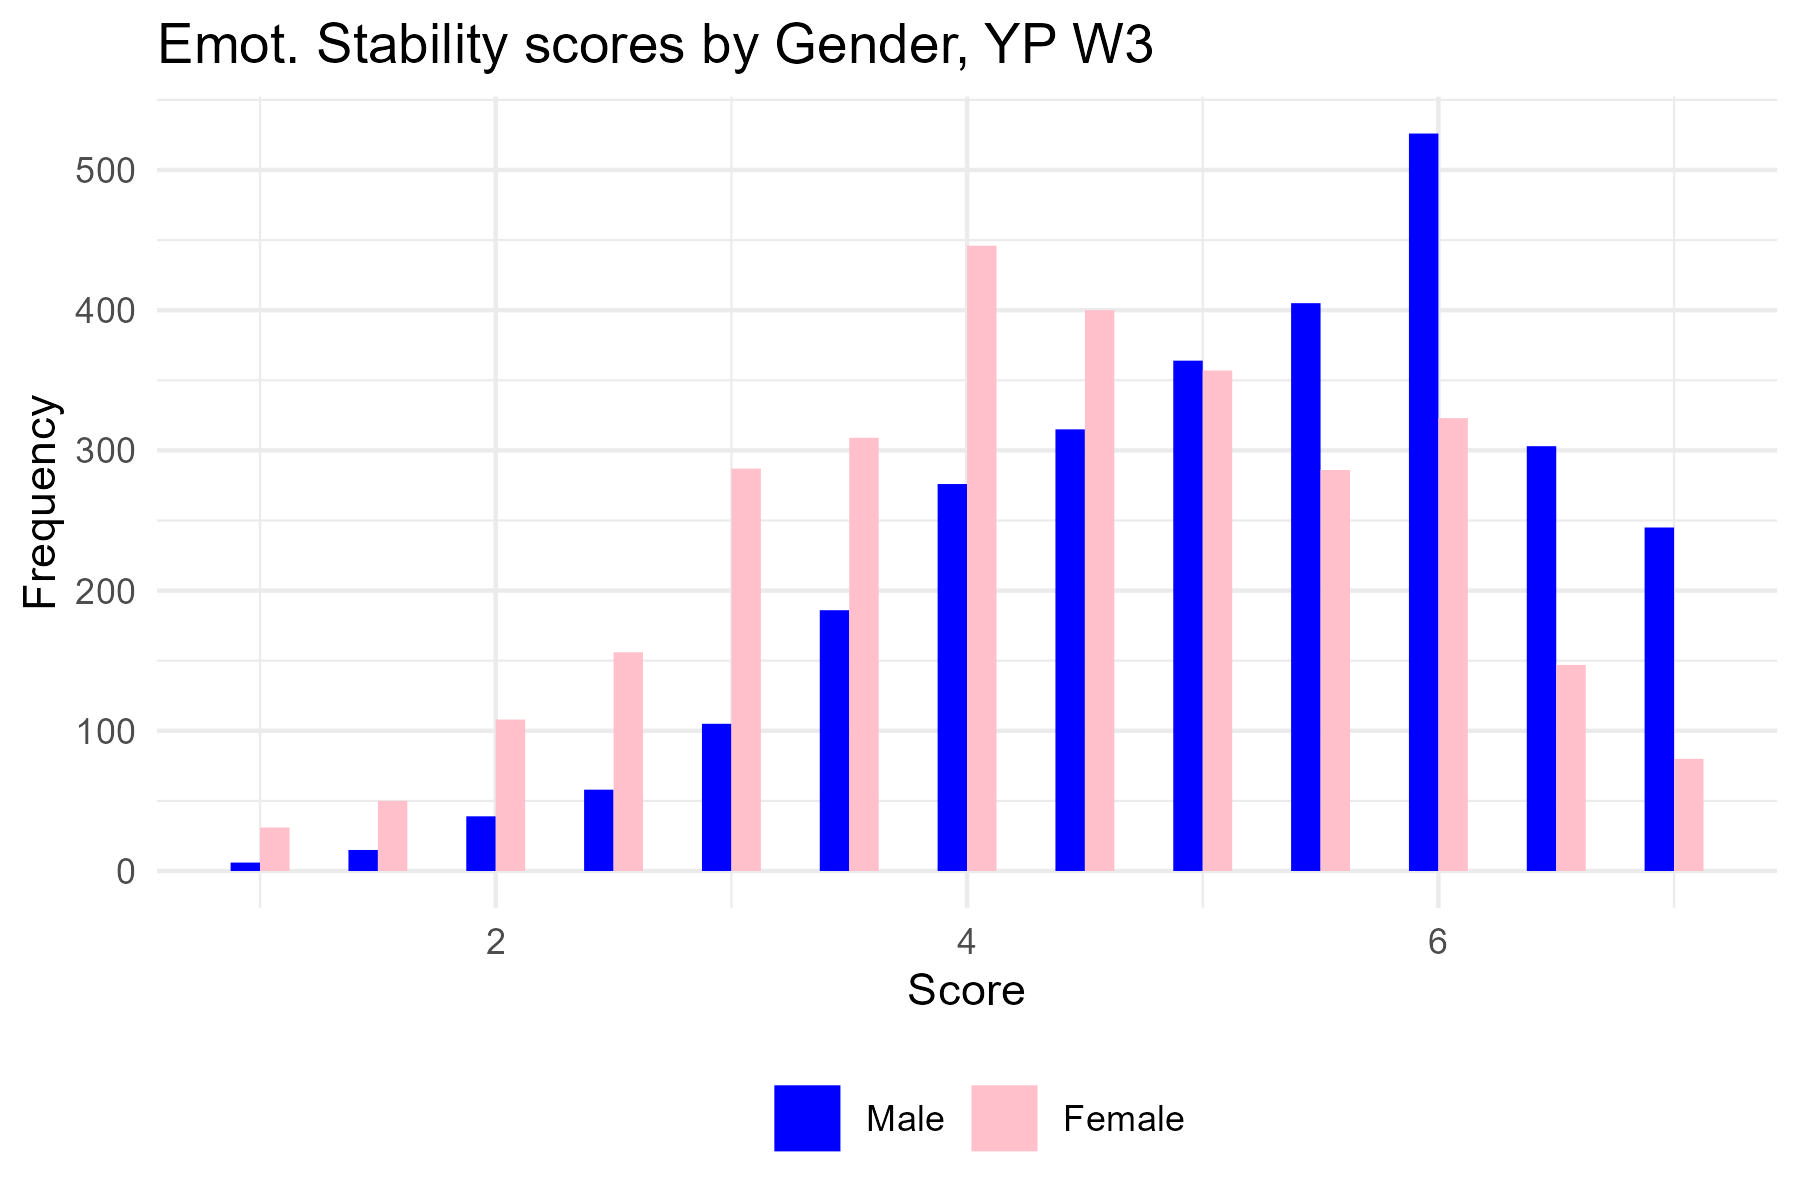
\includegraphics[width=1\linewidth]{Frequency of Emotional Stability Gender.jpeg}
    \caption{Frequency of Emotional Stability scores by gender, reported by YP in wave 3}
    \label{}
\end{figure}

\begin{figure}[htbp] 
    \centering
    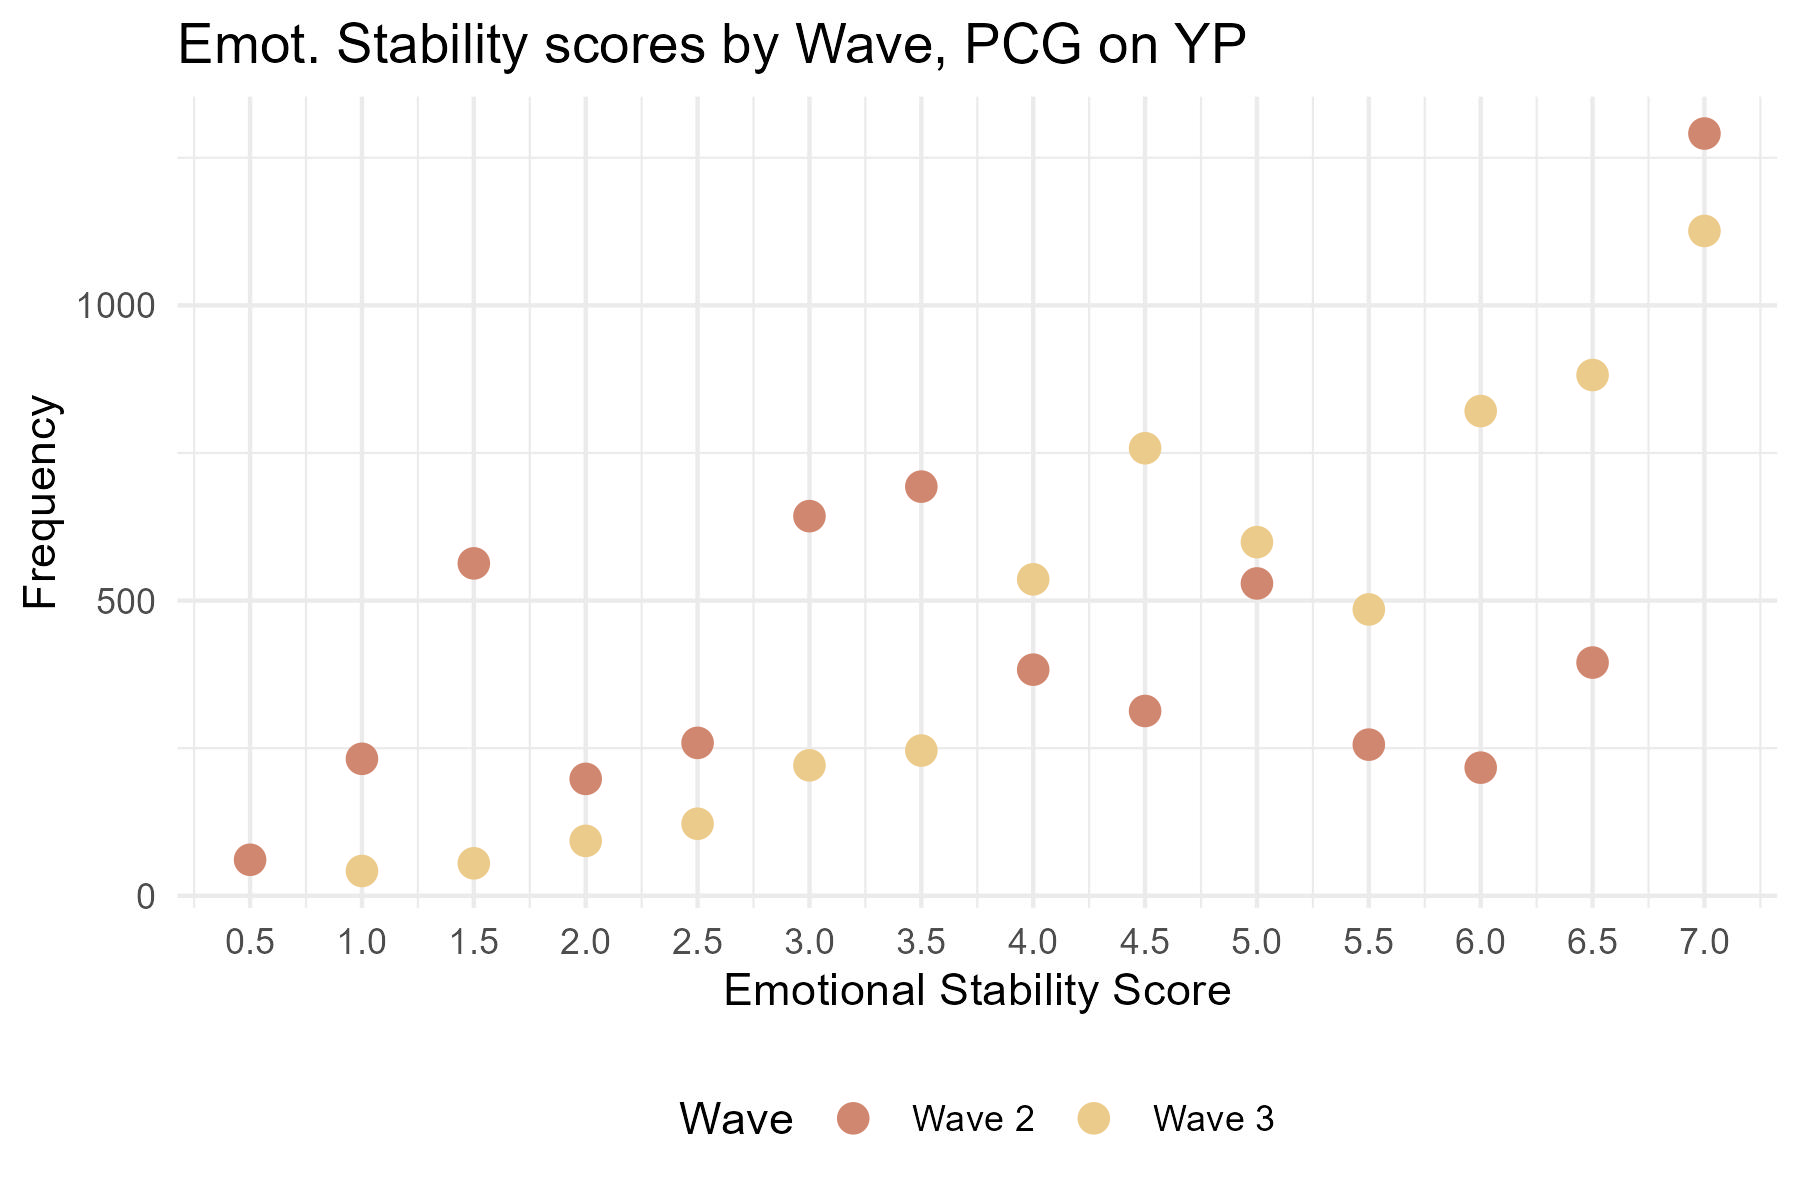
\includegraphics[width=1\linewidth]{Frequency of Emotional Stability by Wave, PCG.jpeg}
    \caption{Frequency of YP's Emotional Stability scores reported by PCG in waves 2 and 3}
    \label{}
\end{figure}

\begin{figure}[htbp] 
    \centering
    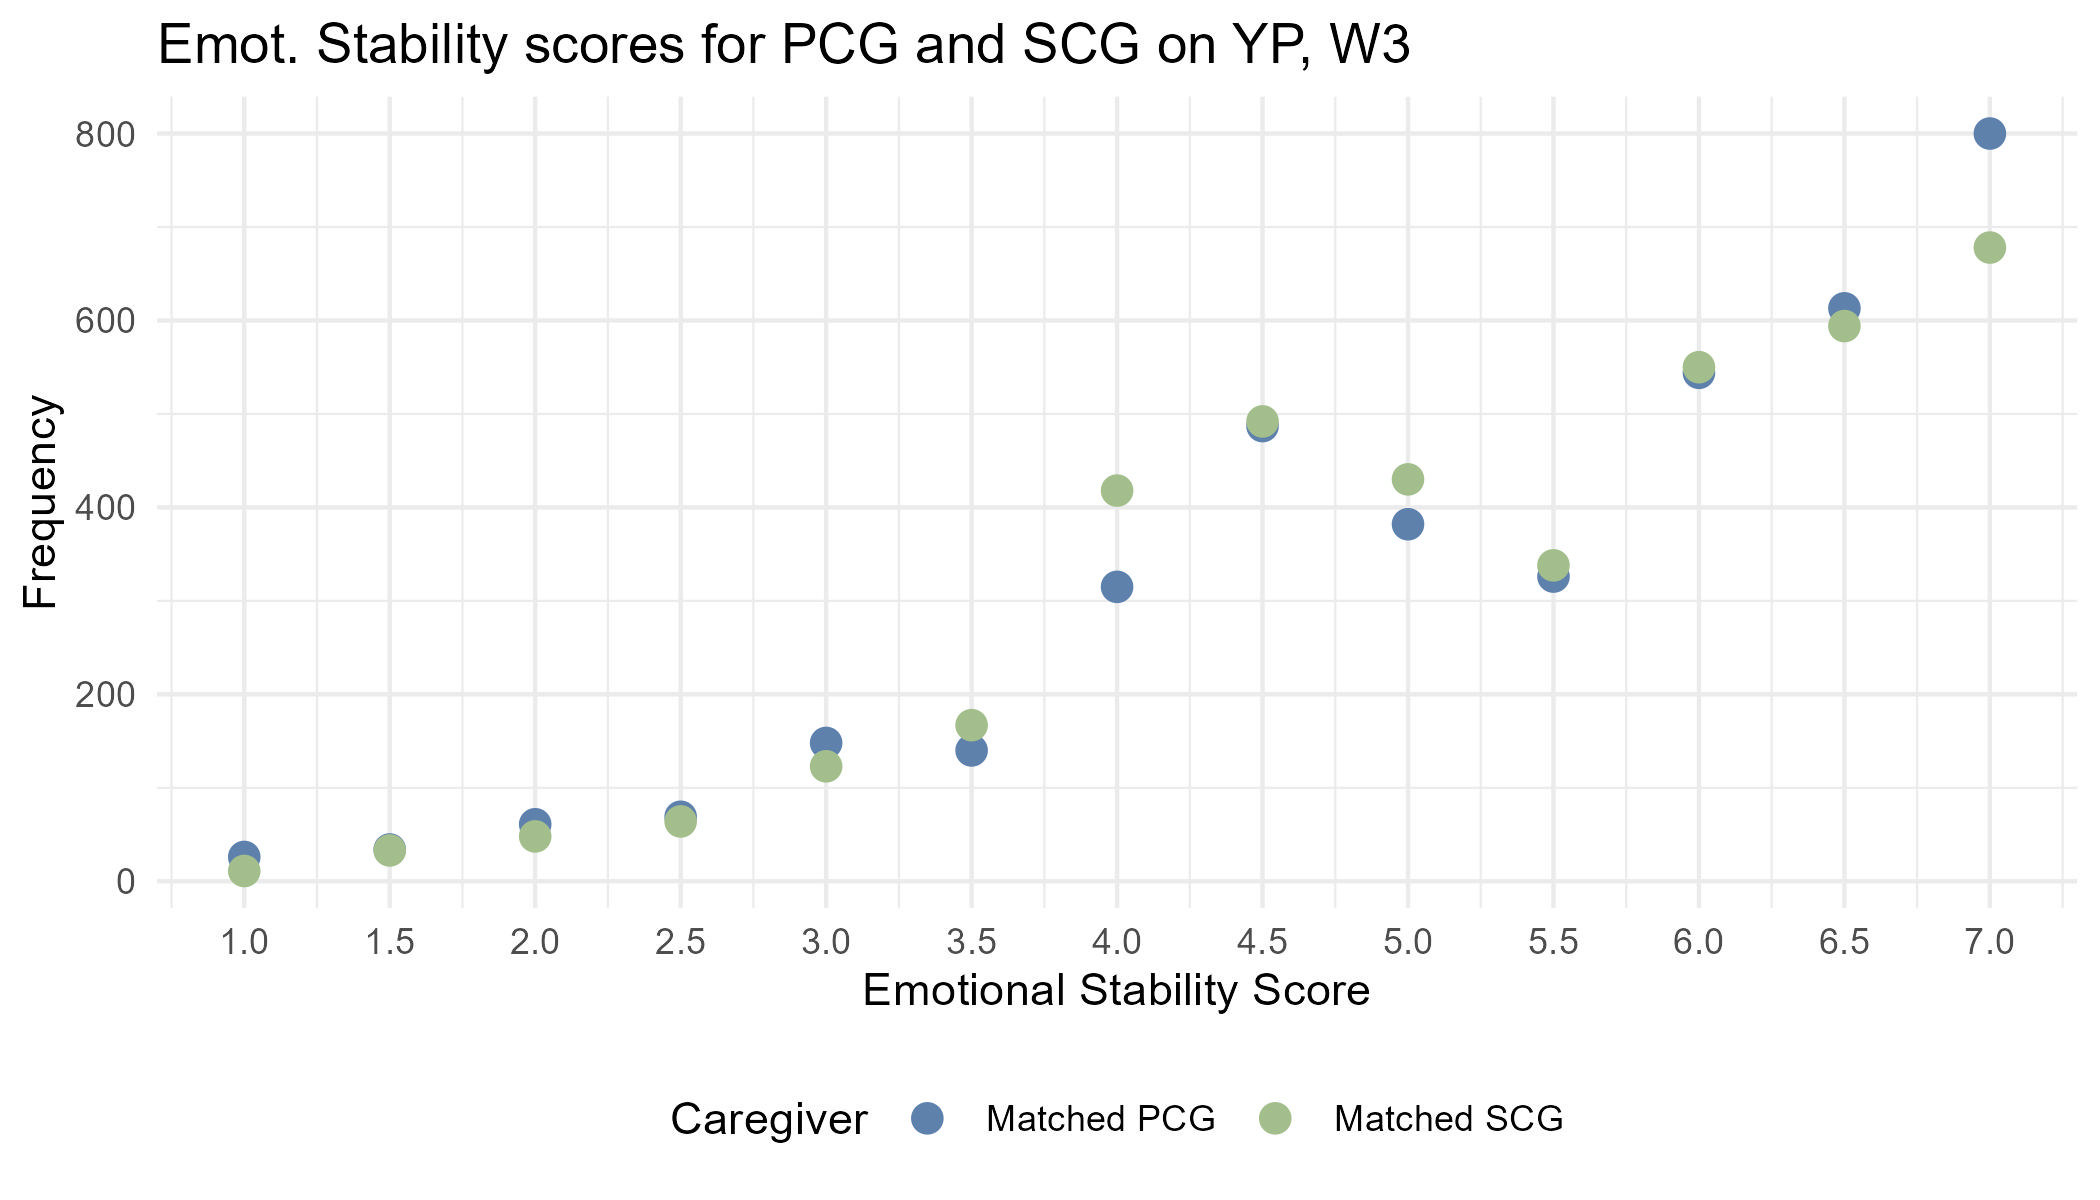
\includegraphics[width=1\linewidth]{Matched Emotional Stability by participant w3.jpeg}
    \caption{Frequency of YP's Emotional Stability scores reported by PCG and SCG in wave 3 (matched)}
    \label{}
\end{figure}


\begin{figure}[htbp] 
    \centering
    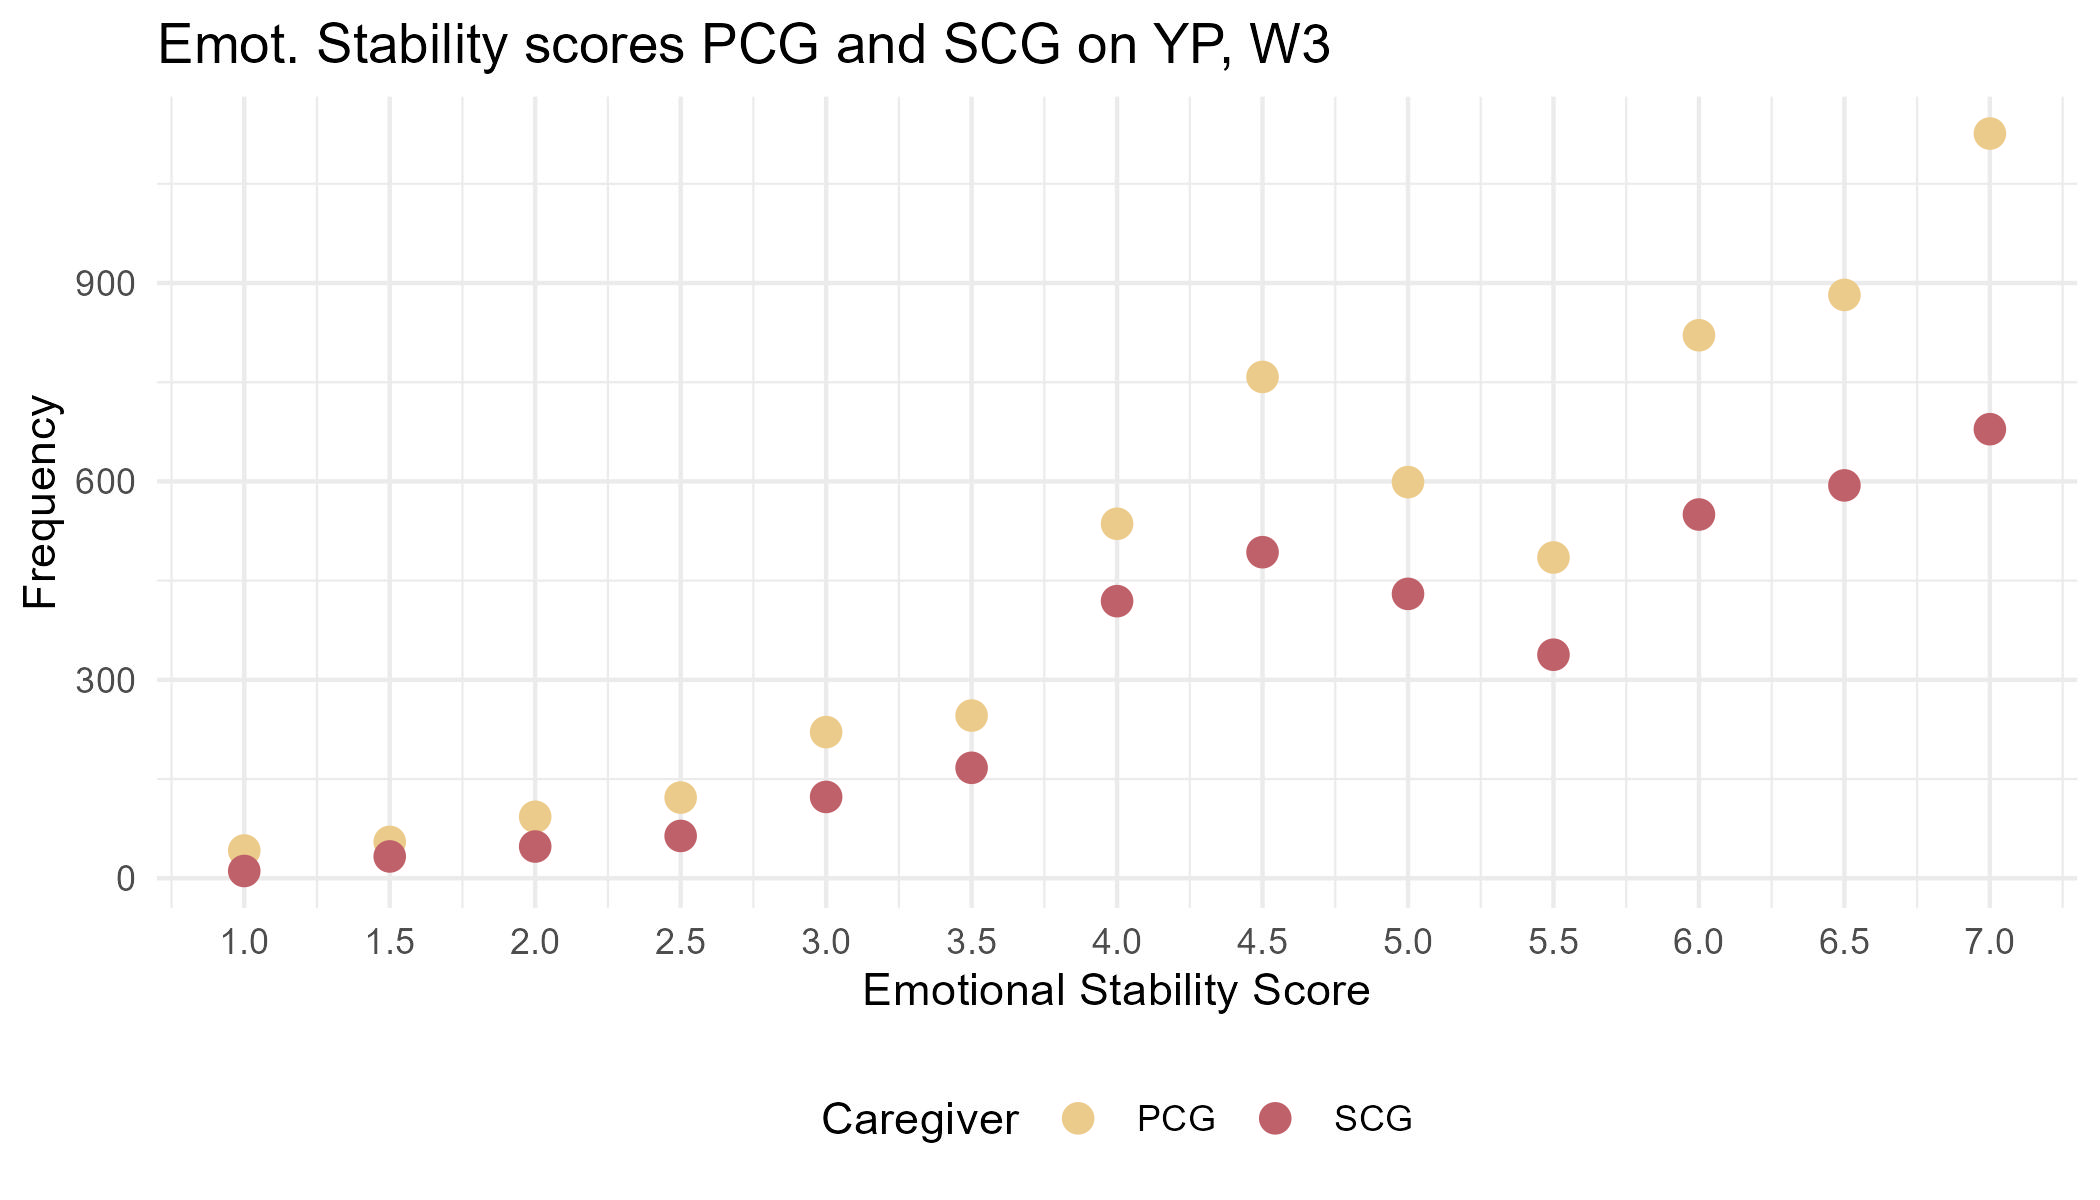
\includegraphics[width=1\linewidth]{Frequency of Emotional Stability by participant w3.jpeg}
    \caption{Frequency of YP's Emotional Stability scores reported by PCG and SCG in wave 3 (not matched}
    \label{}
\end{figure}

\begin{figure}[htbp] 
    \centering
    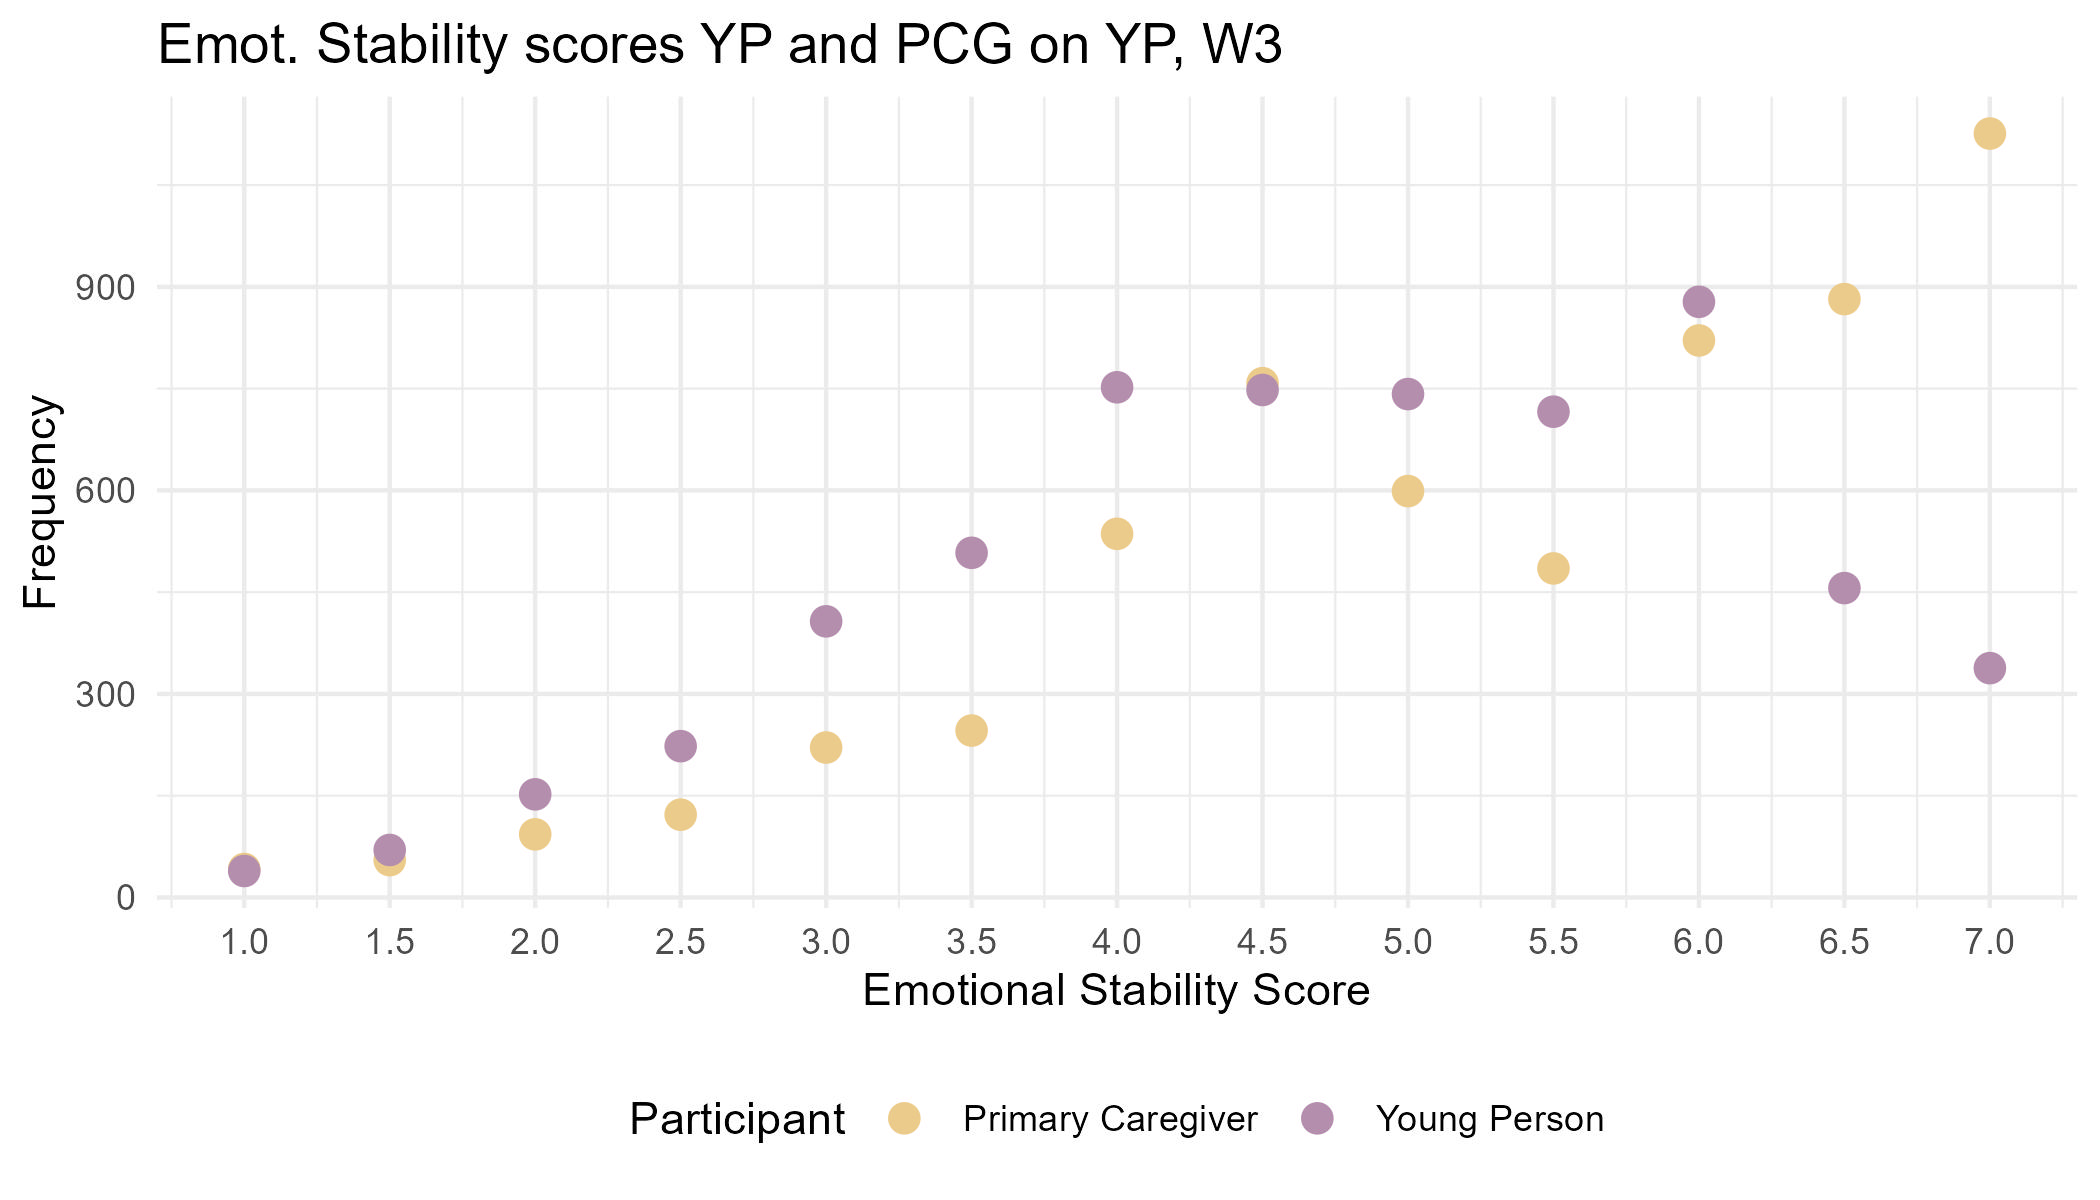
\includegraphics[width=1\linewidth]{Frequency of Emotional Stability by participant w3a.jpeg}
    \caption{Frequency of YP's Emotional Stability scores reported by YP and PCG in wave 3}
    \label{}
\end{figure}

\begin{figure}[htbp] 
    \centering
    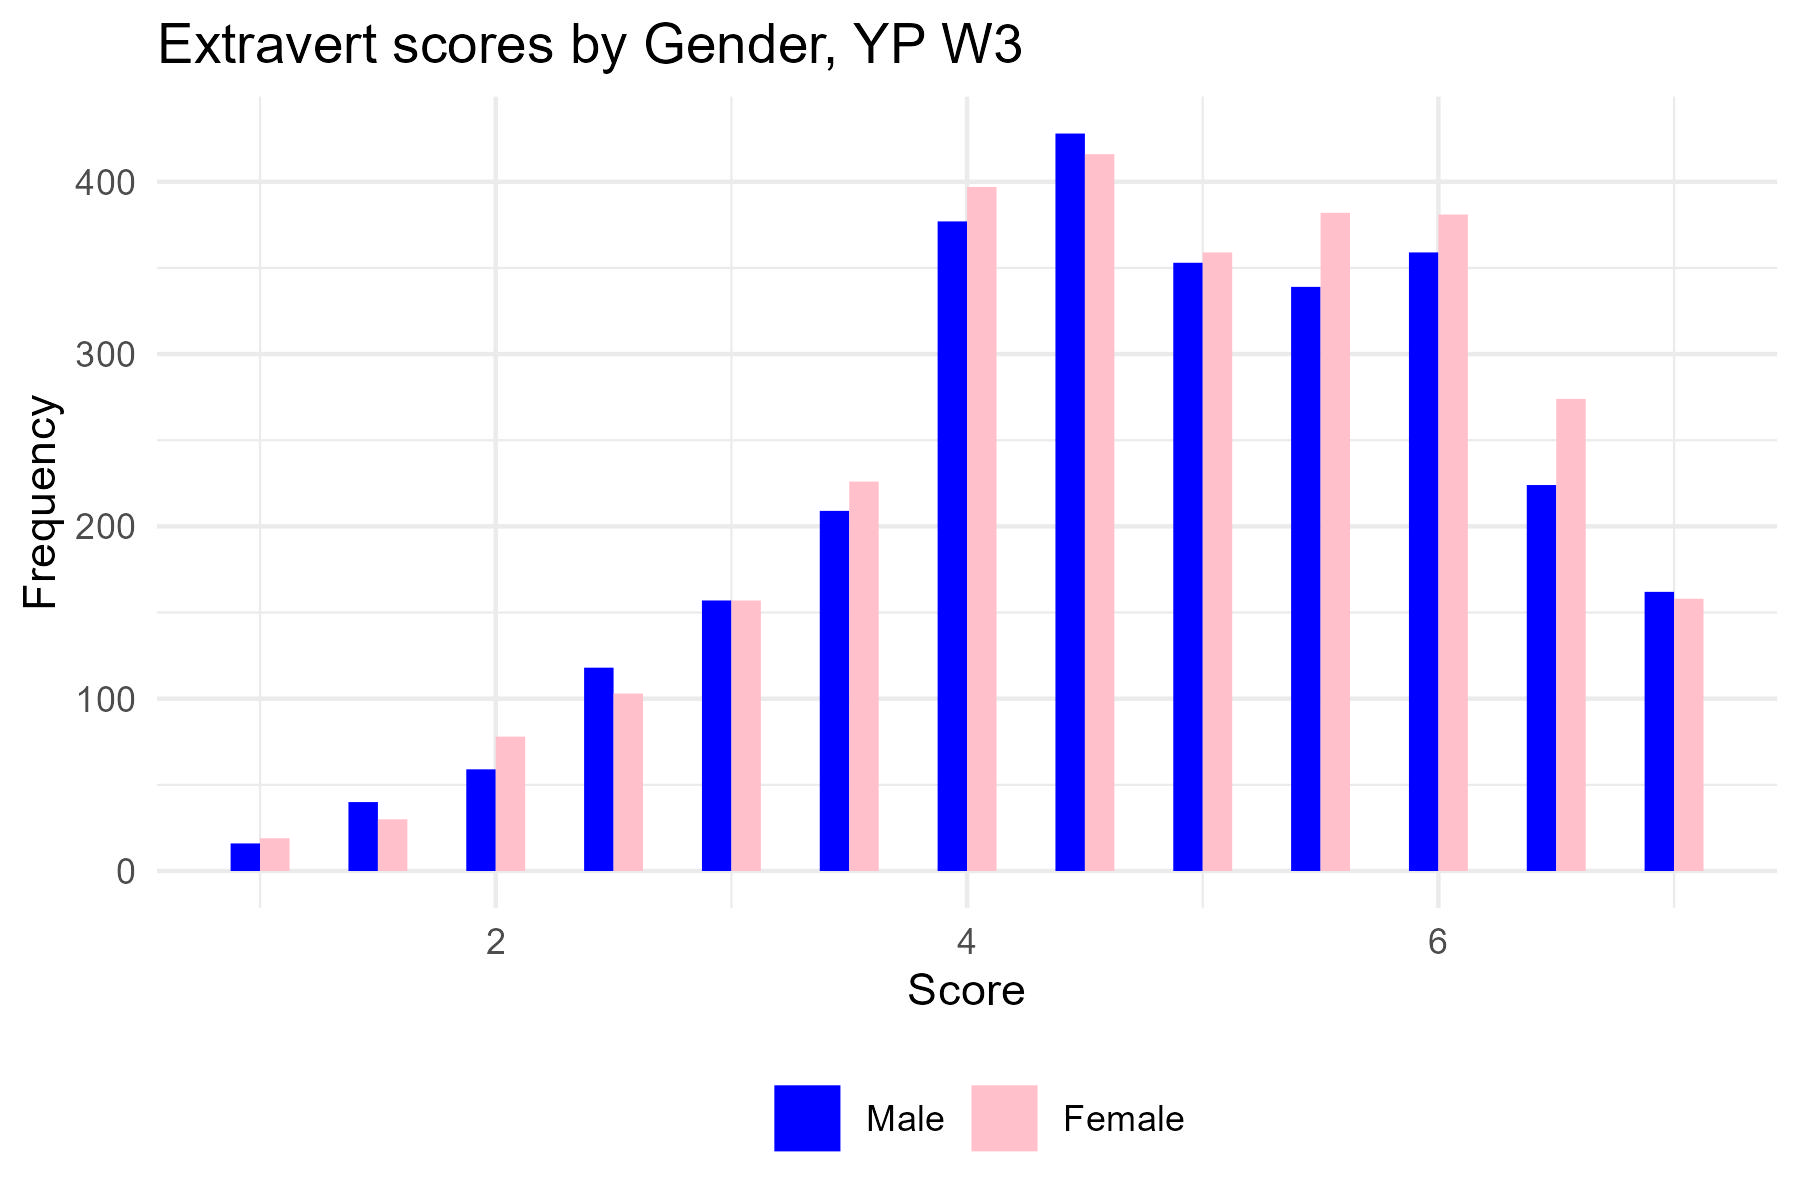
\includegraphics[width=1\linewidth]{Frequency of Extravert by Gender.jpeg}
    \caption{Frequency of Extravert scores by gender, reported by YP in wave 3}
    \label{}
\end{figure}

\begin{figure}[htbp] 
    \centering
    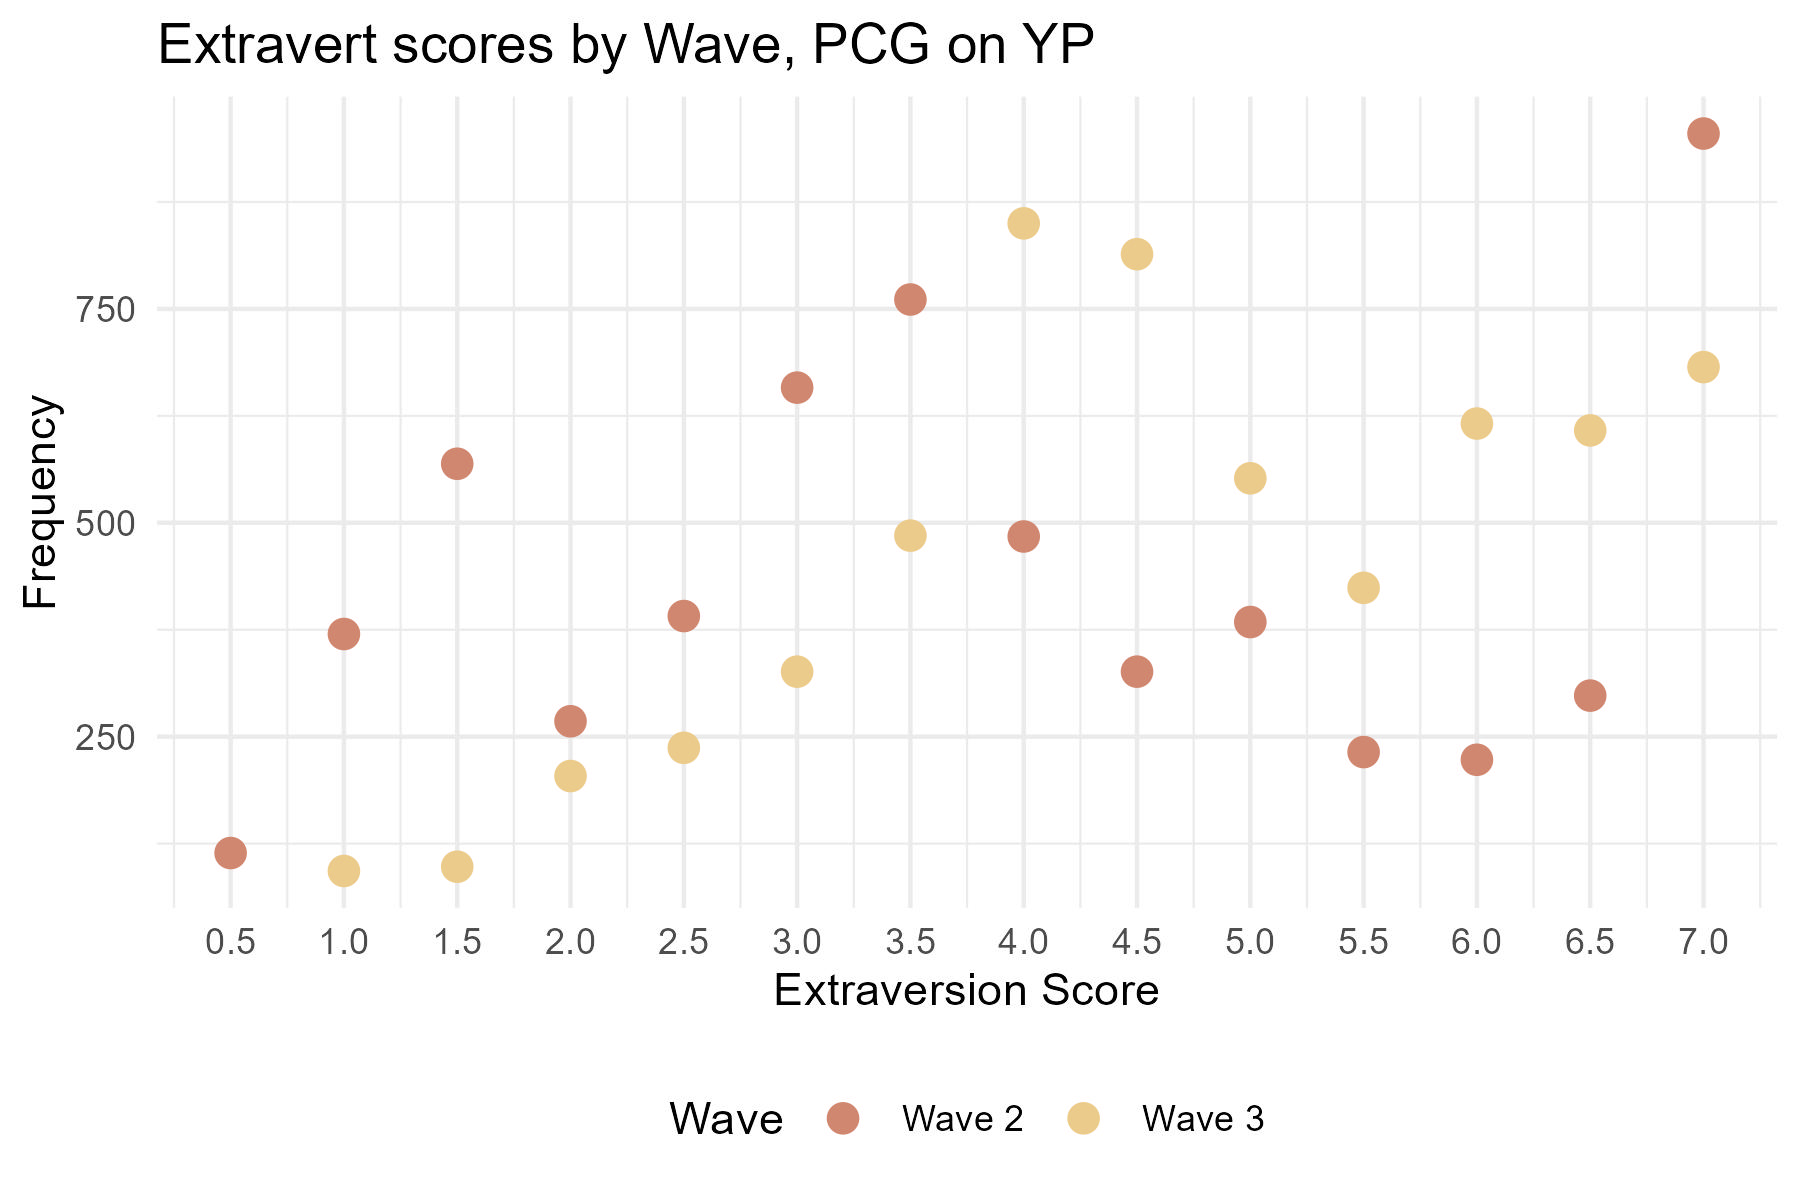
\includegraphics[width=1\linewidth]{Frequency of Extravert by Wave, PCG.jpeg}
    \caption{Frequency of YP's Extravert scores reported by PCG in waves 2 and 3}
    \label{}
\end{figure}

\begin{figure}[htbp] 
    \centering
    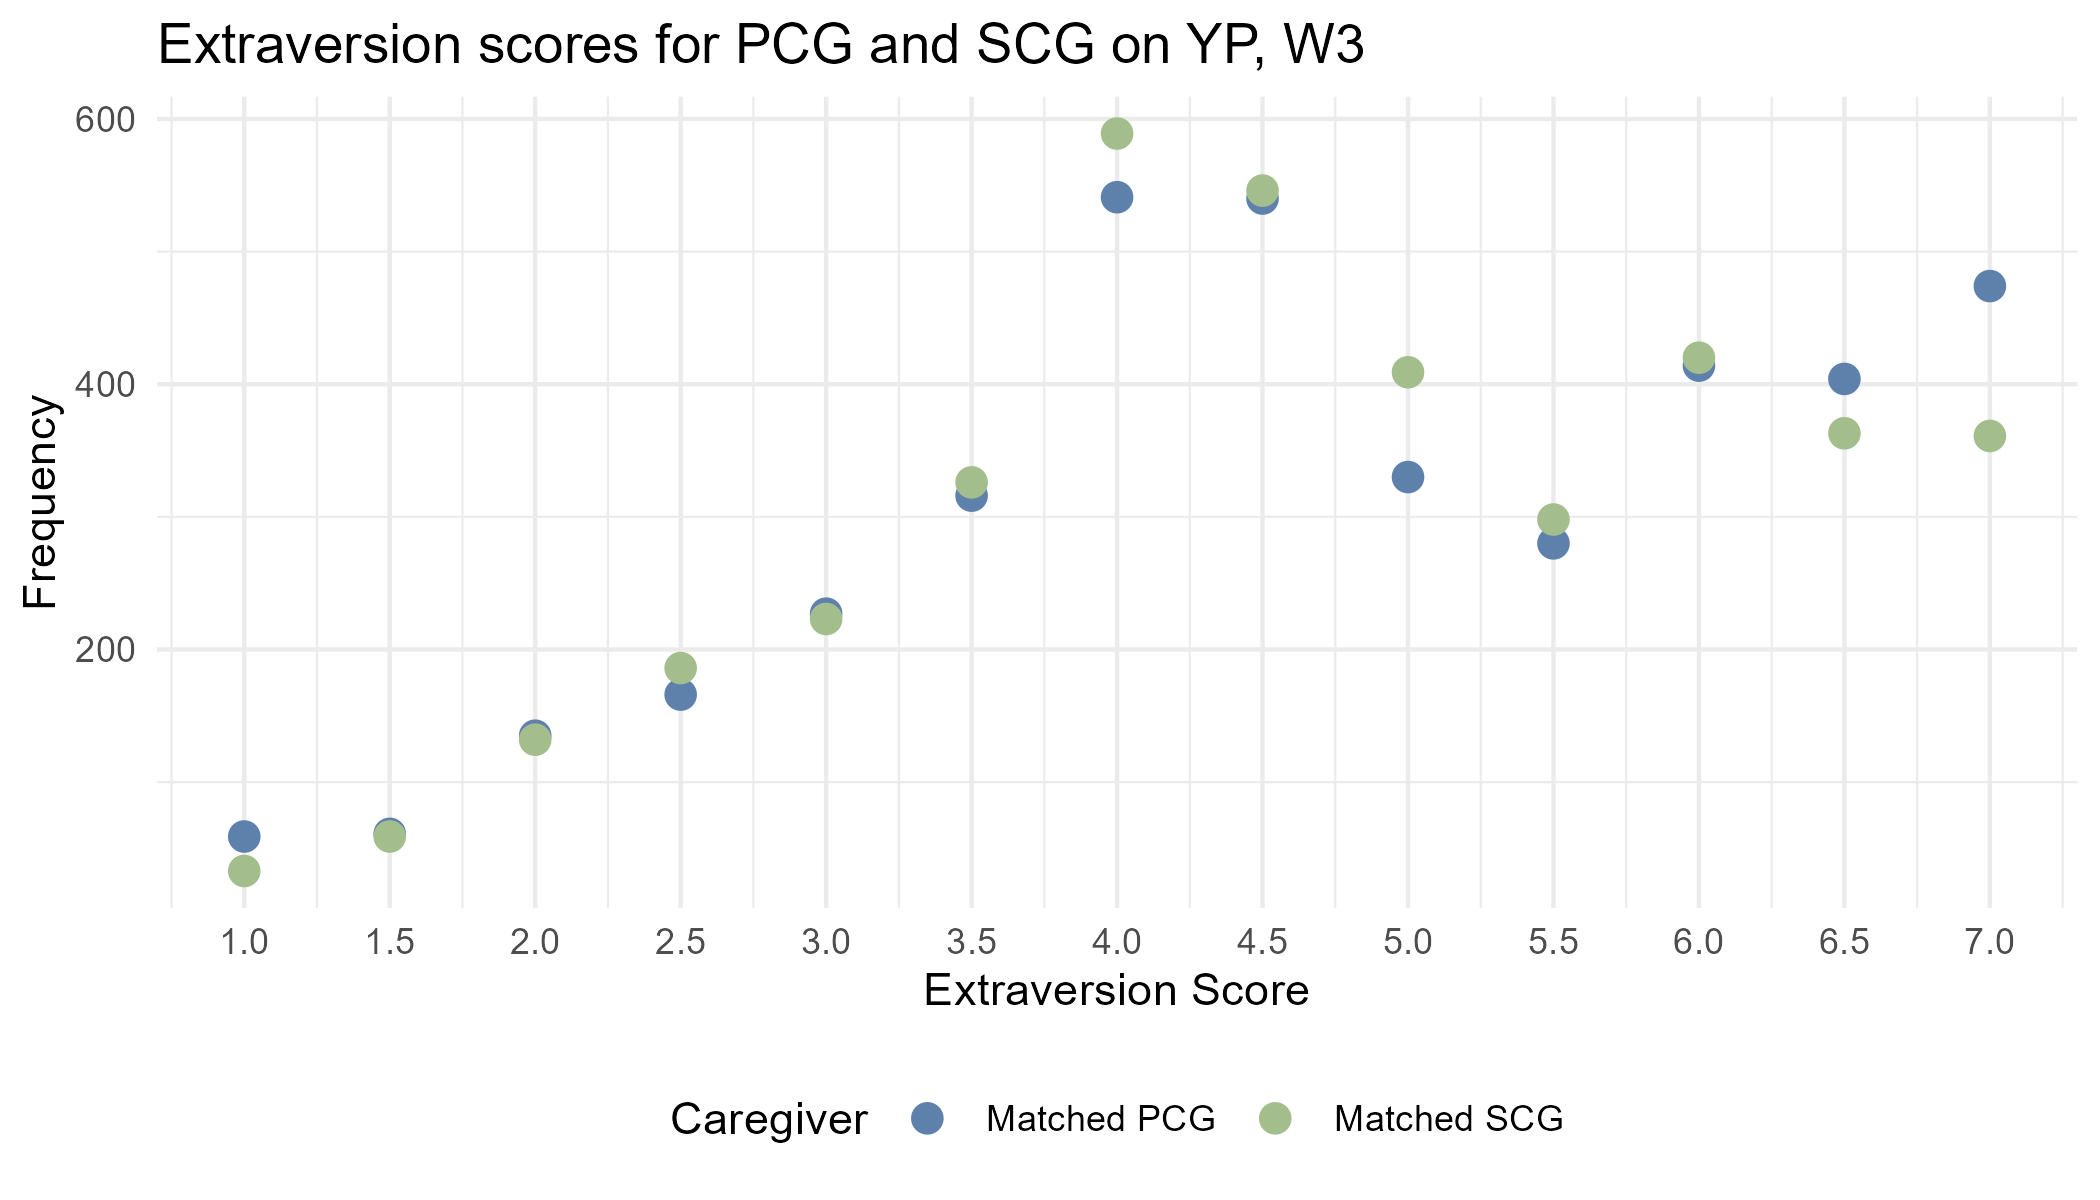
\includegraphics[width=1\linewidth]{Matched Extravert by participant w3.jpeg}
    \caption{Frequency of YP's Extravert scores reported by PCG and SCG in wave 3 (matched)}
    \label{}
\end{figure}

\begin{figure}[htbp] 
    \centering
    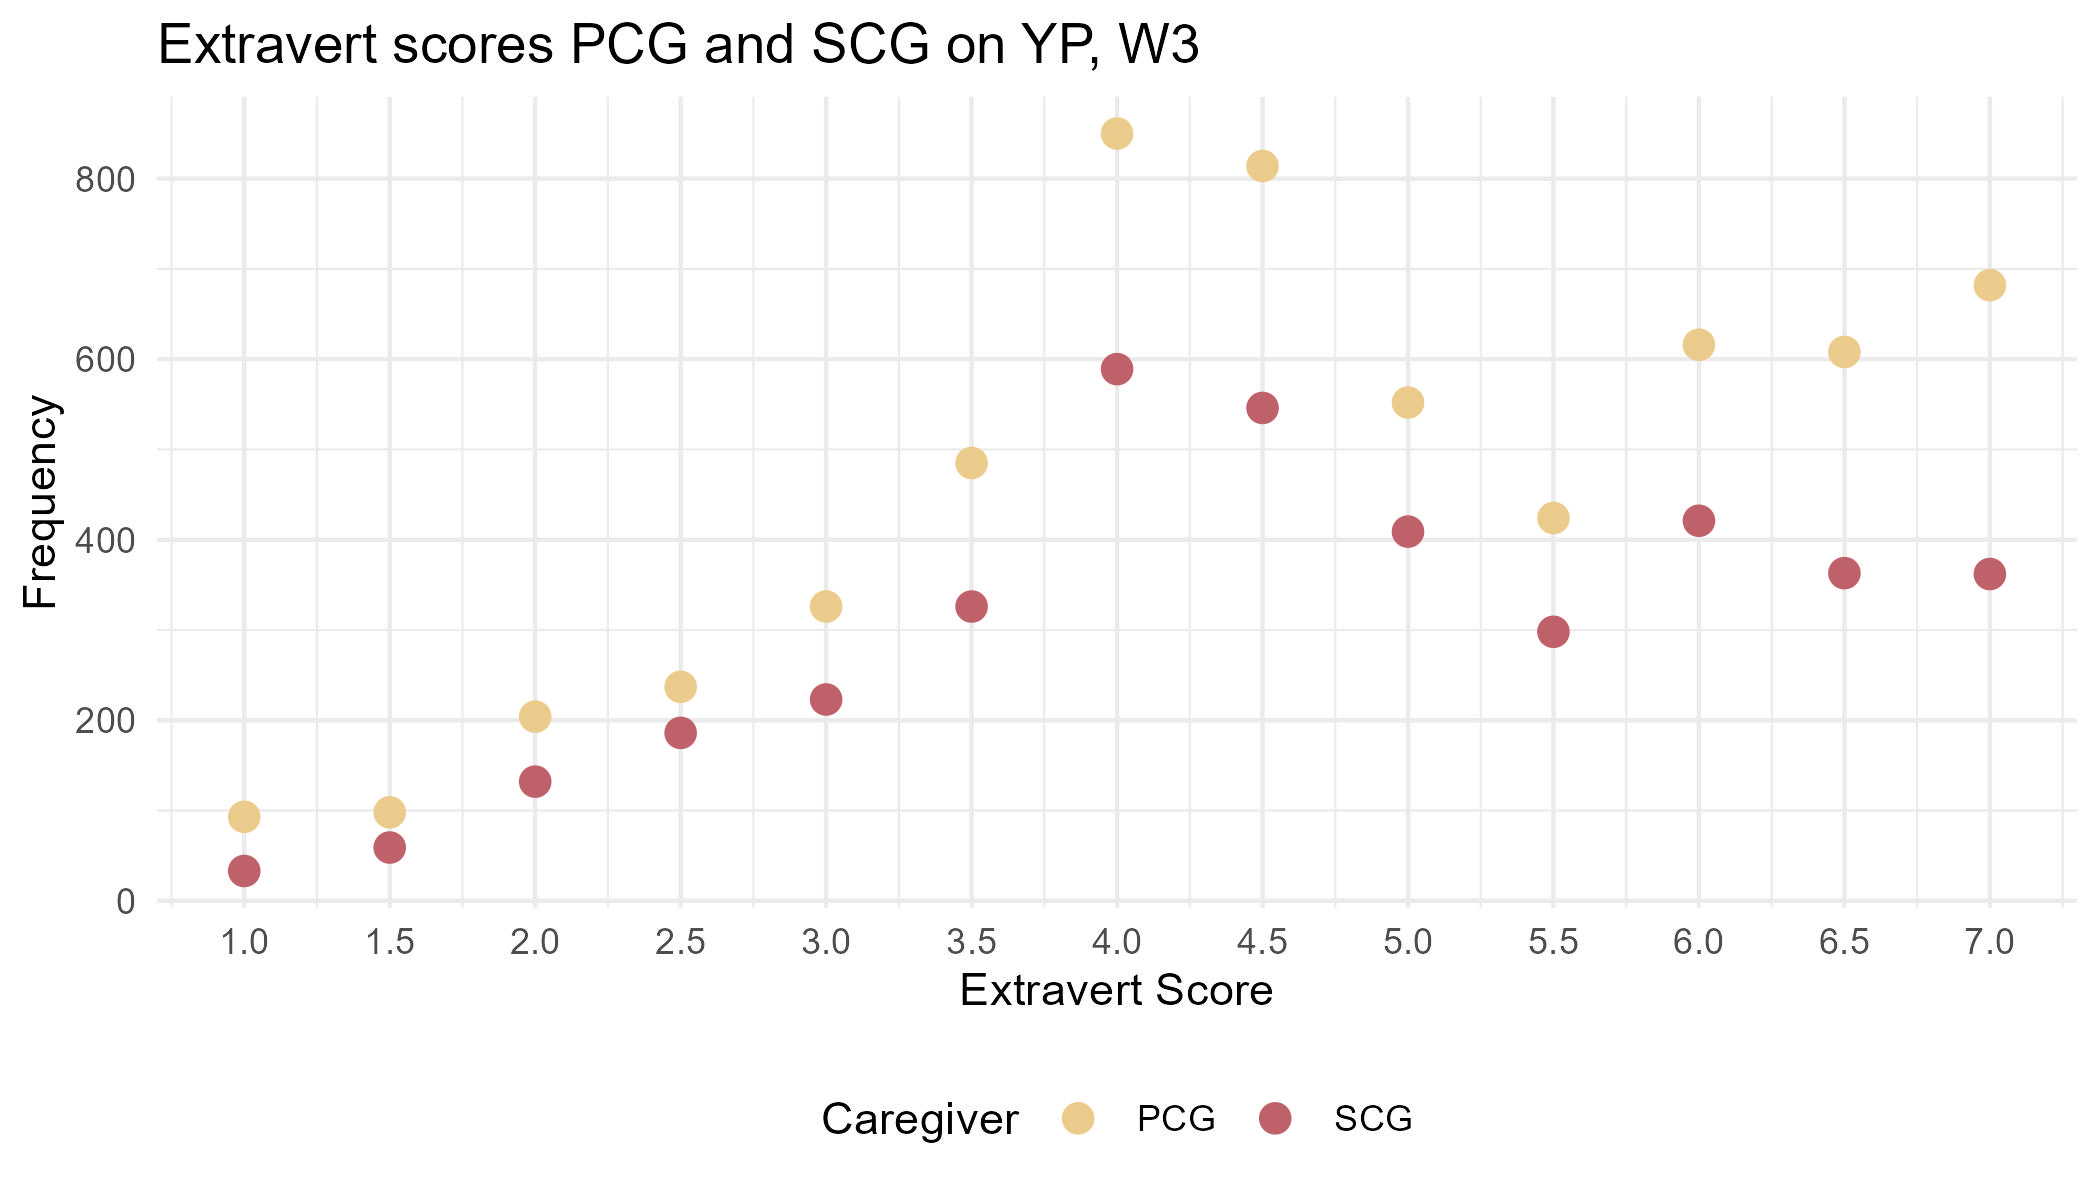
\includegraphics[width=1\linewidth]{Frequency of Extravert by participant w3.jpeg}
    \caption{Frequency of YP's Extravert scores reported by PCG and SCG in wave 3 (not matched}
    \label{}
\end{figure}

\begin{figure}[htbp] 
    \centering
    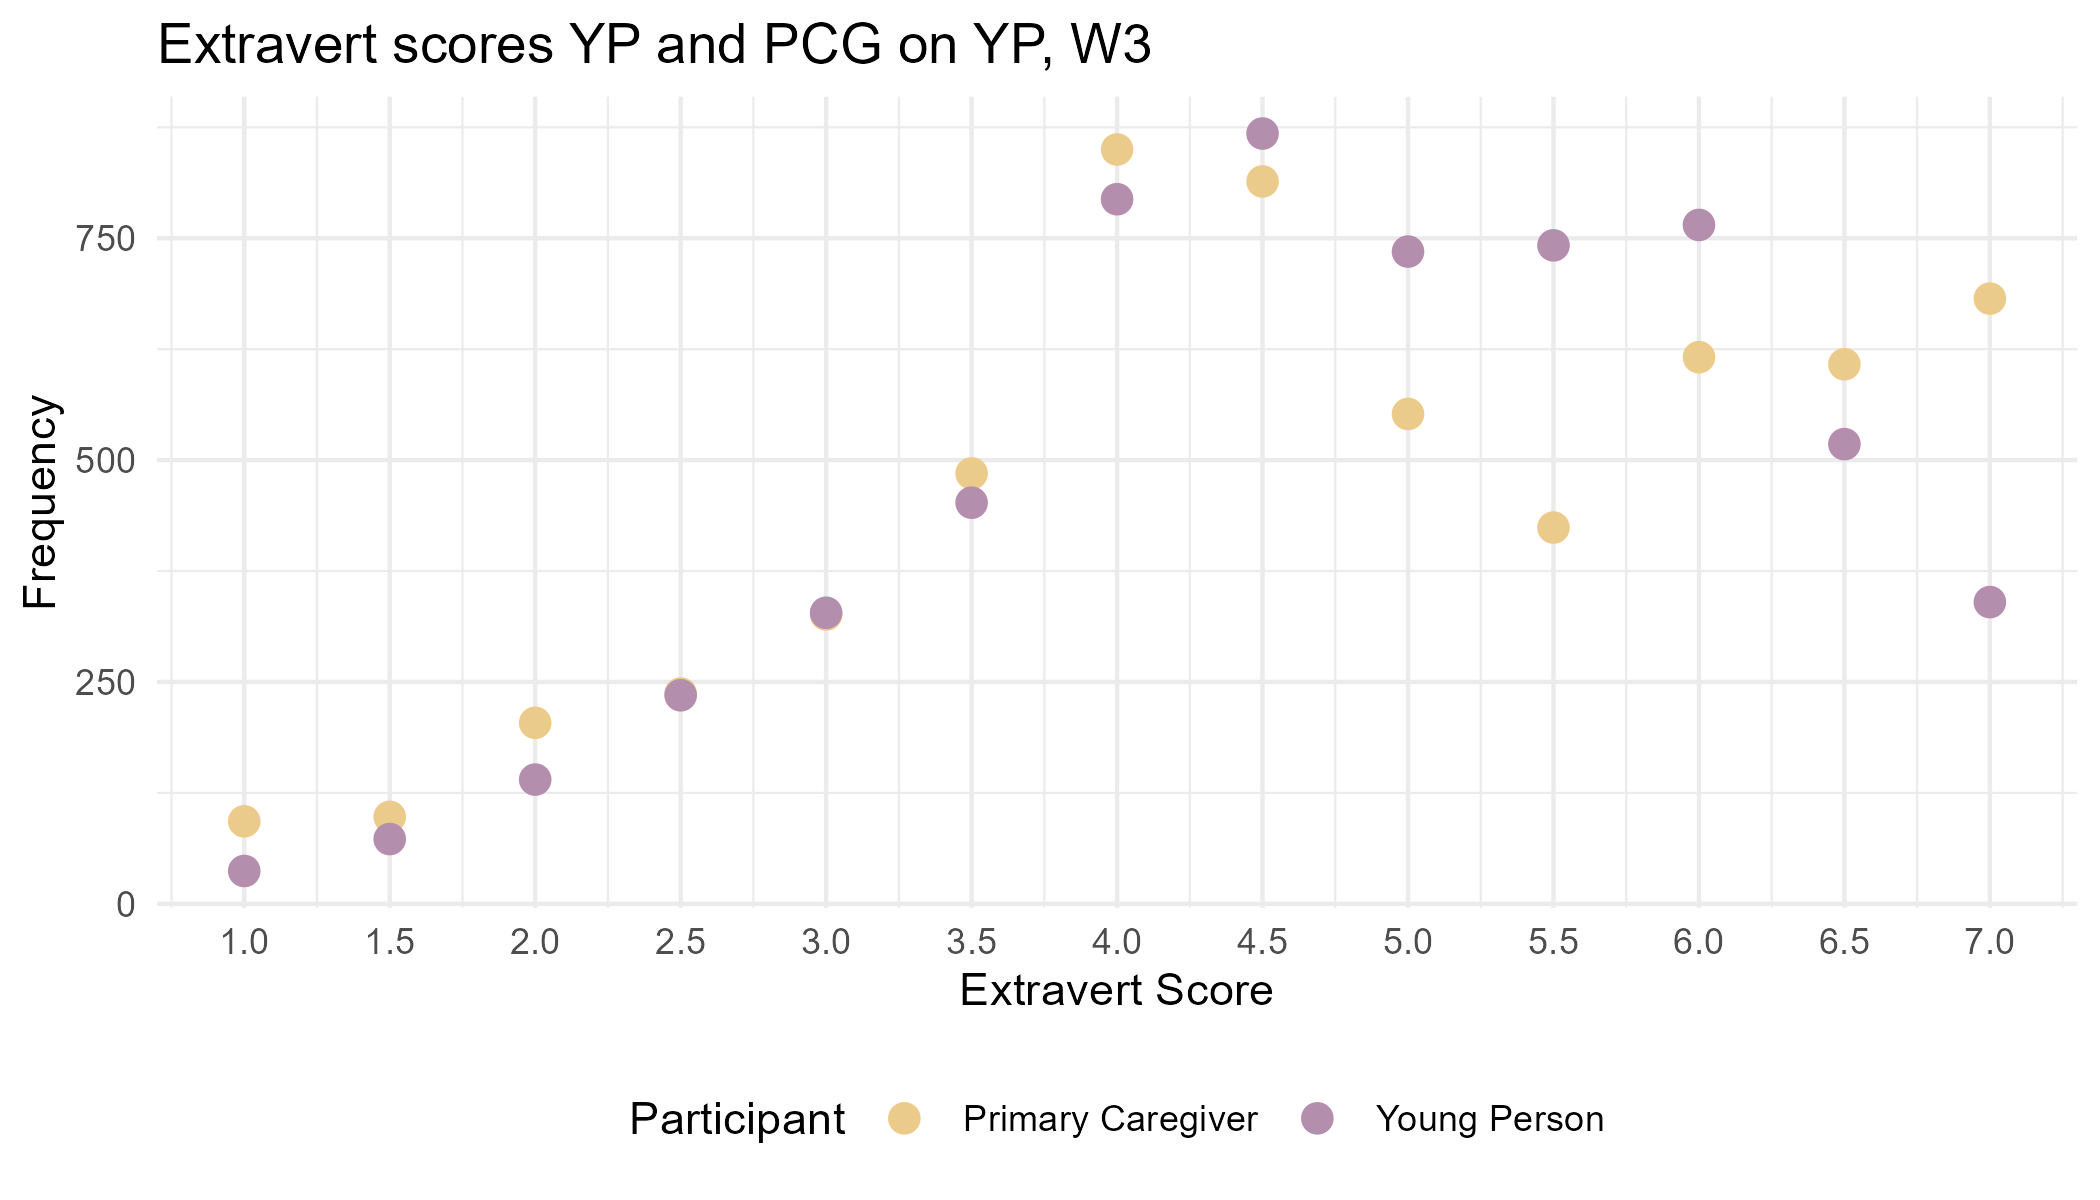
\includegraphics[width=1\linewidth]{Frequency of Extravert by participant w3a.jpeg}
    \caption{Frequency of YP's Extravert scores reported by YP and PCG in wave 3}
    \label{}
\end{figure}



\begin{figure}[htbp] 
    \centering
    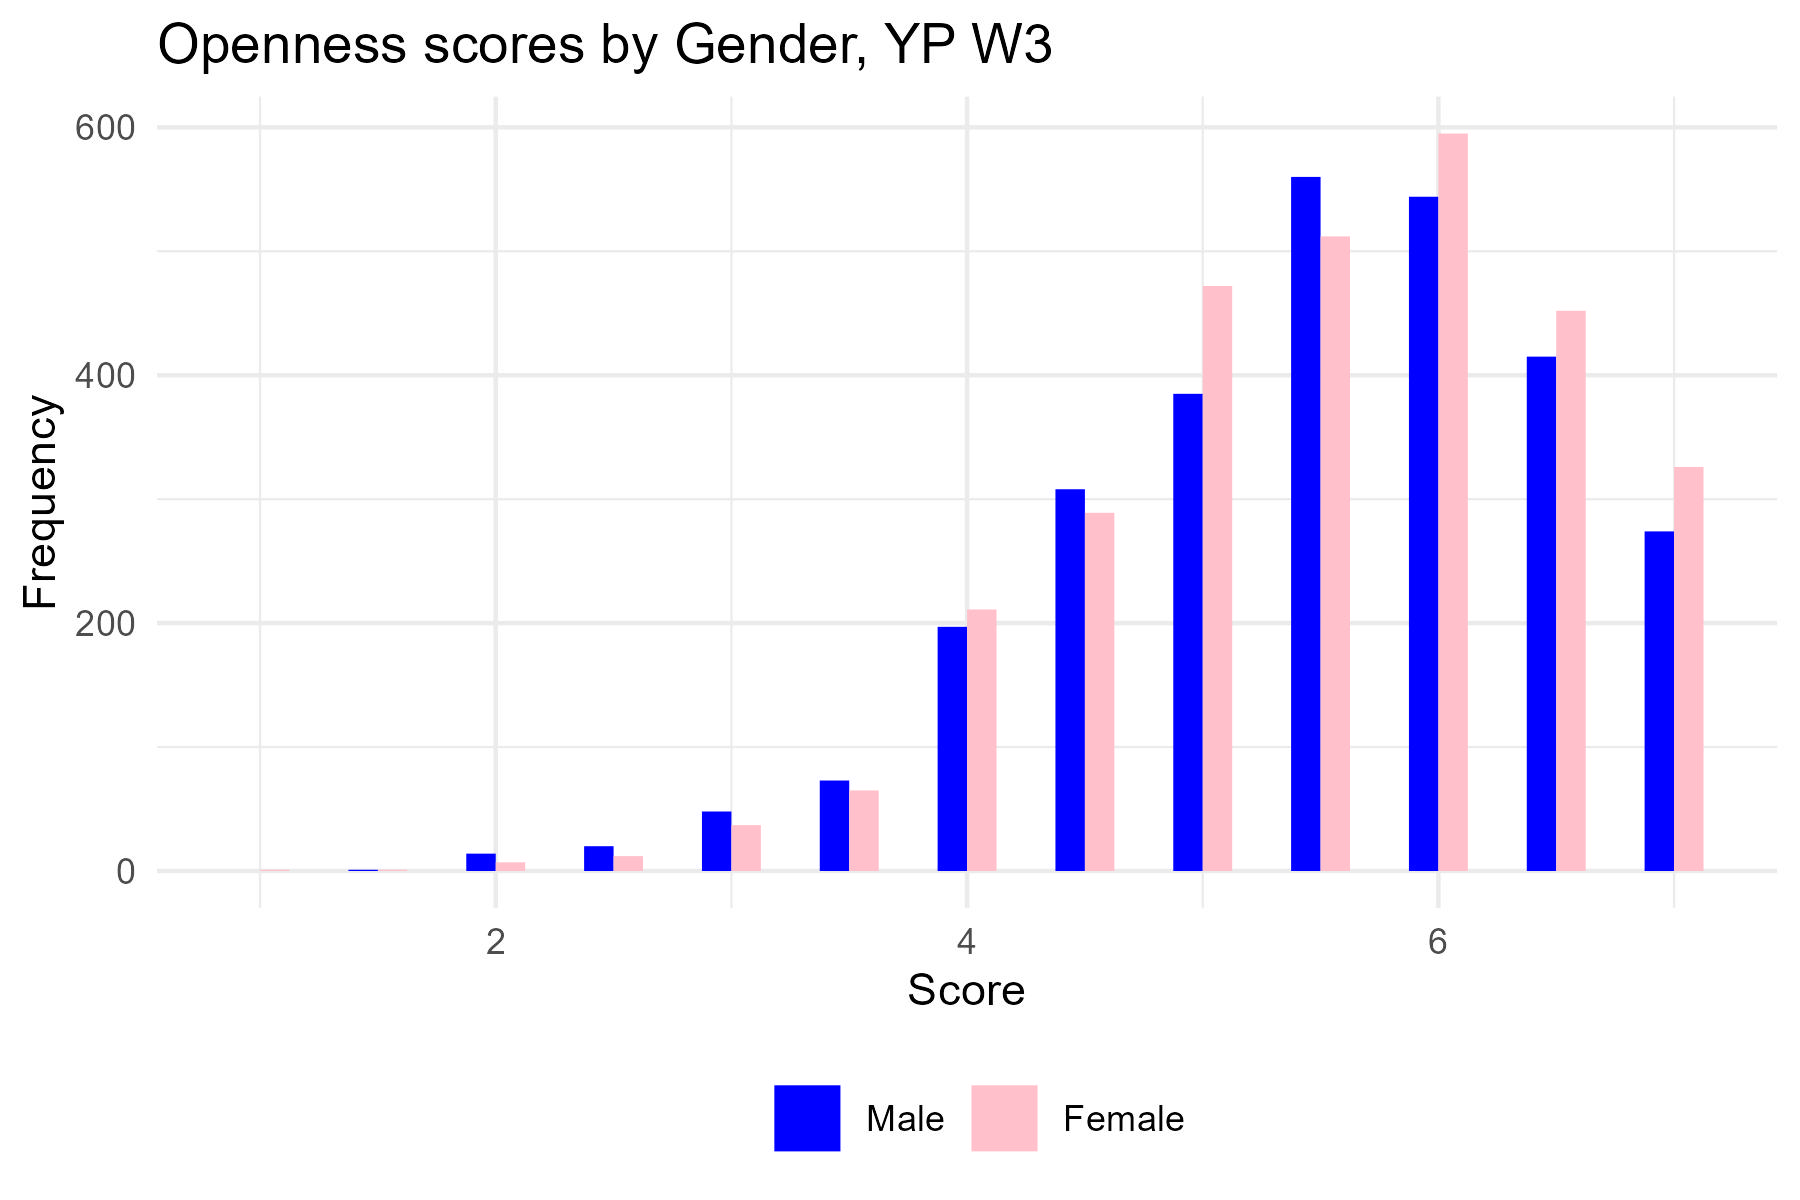
\includegraphics[width=1\linewidth]{Frequency of Openness by Gender side by side.jpeg}
    \caption{Frequency of Openness scores by gender, reported by YP in wave 3}
    \label{}
\end{figure}

\begin{figure}[htbp] 
    \centering
    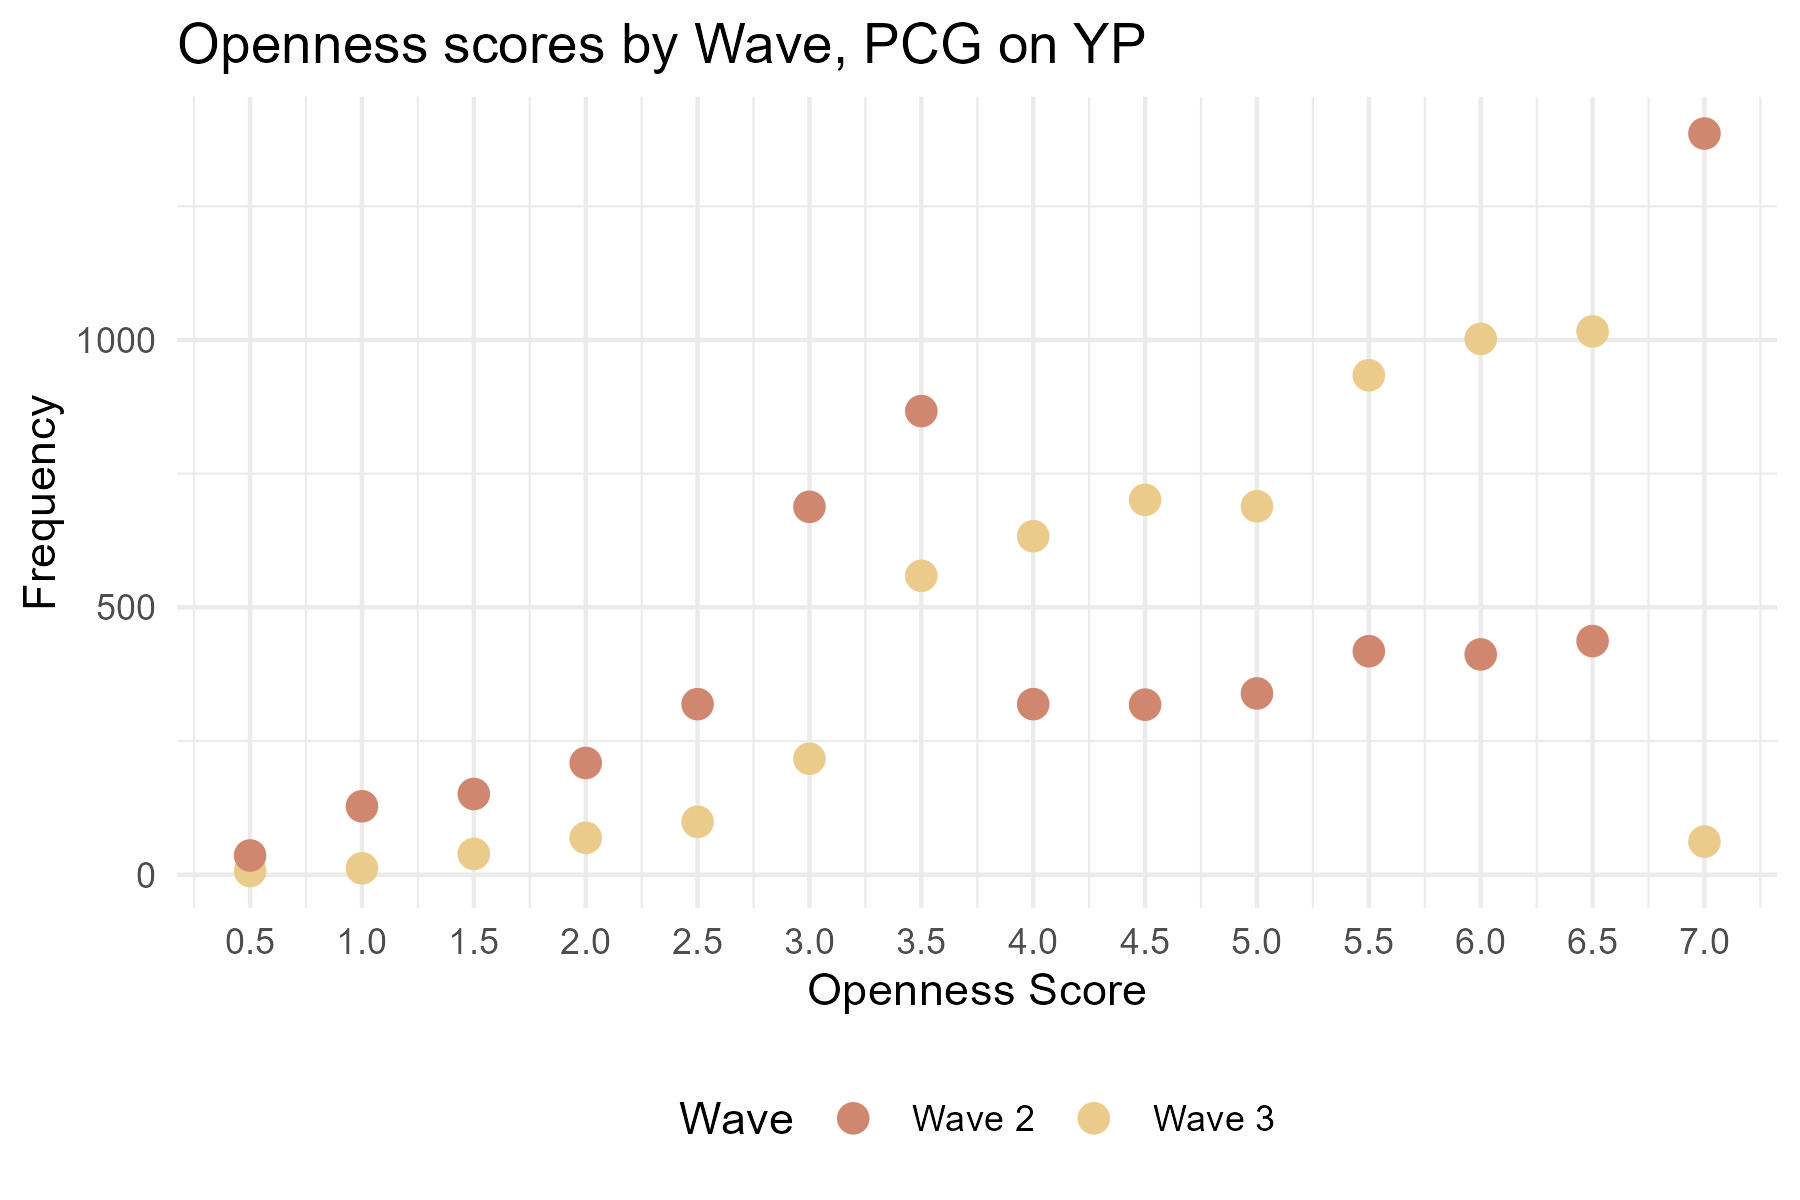
\includegraphics[width=1\linewidth]{Frequency of Openness by Wave, PCG.jpeg}
    \caption{Frequency of YP's Openness scores reported by PCG in waves 2 and 3}
    \label{}
\end{figure}

\begin{figure}[htbp] 
    \centering
    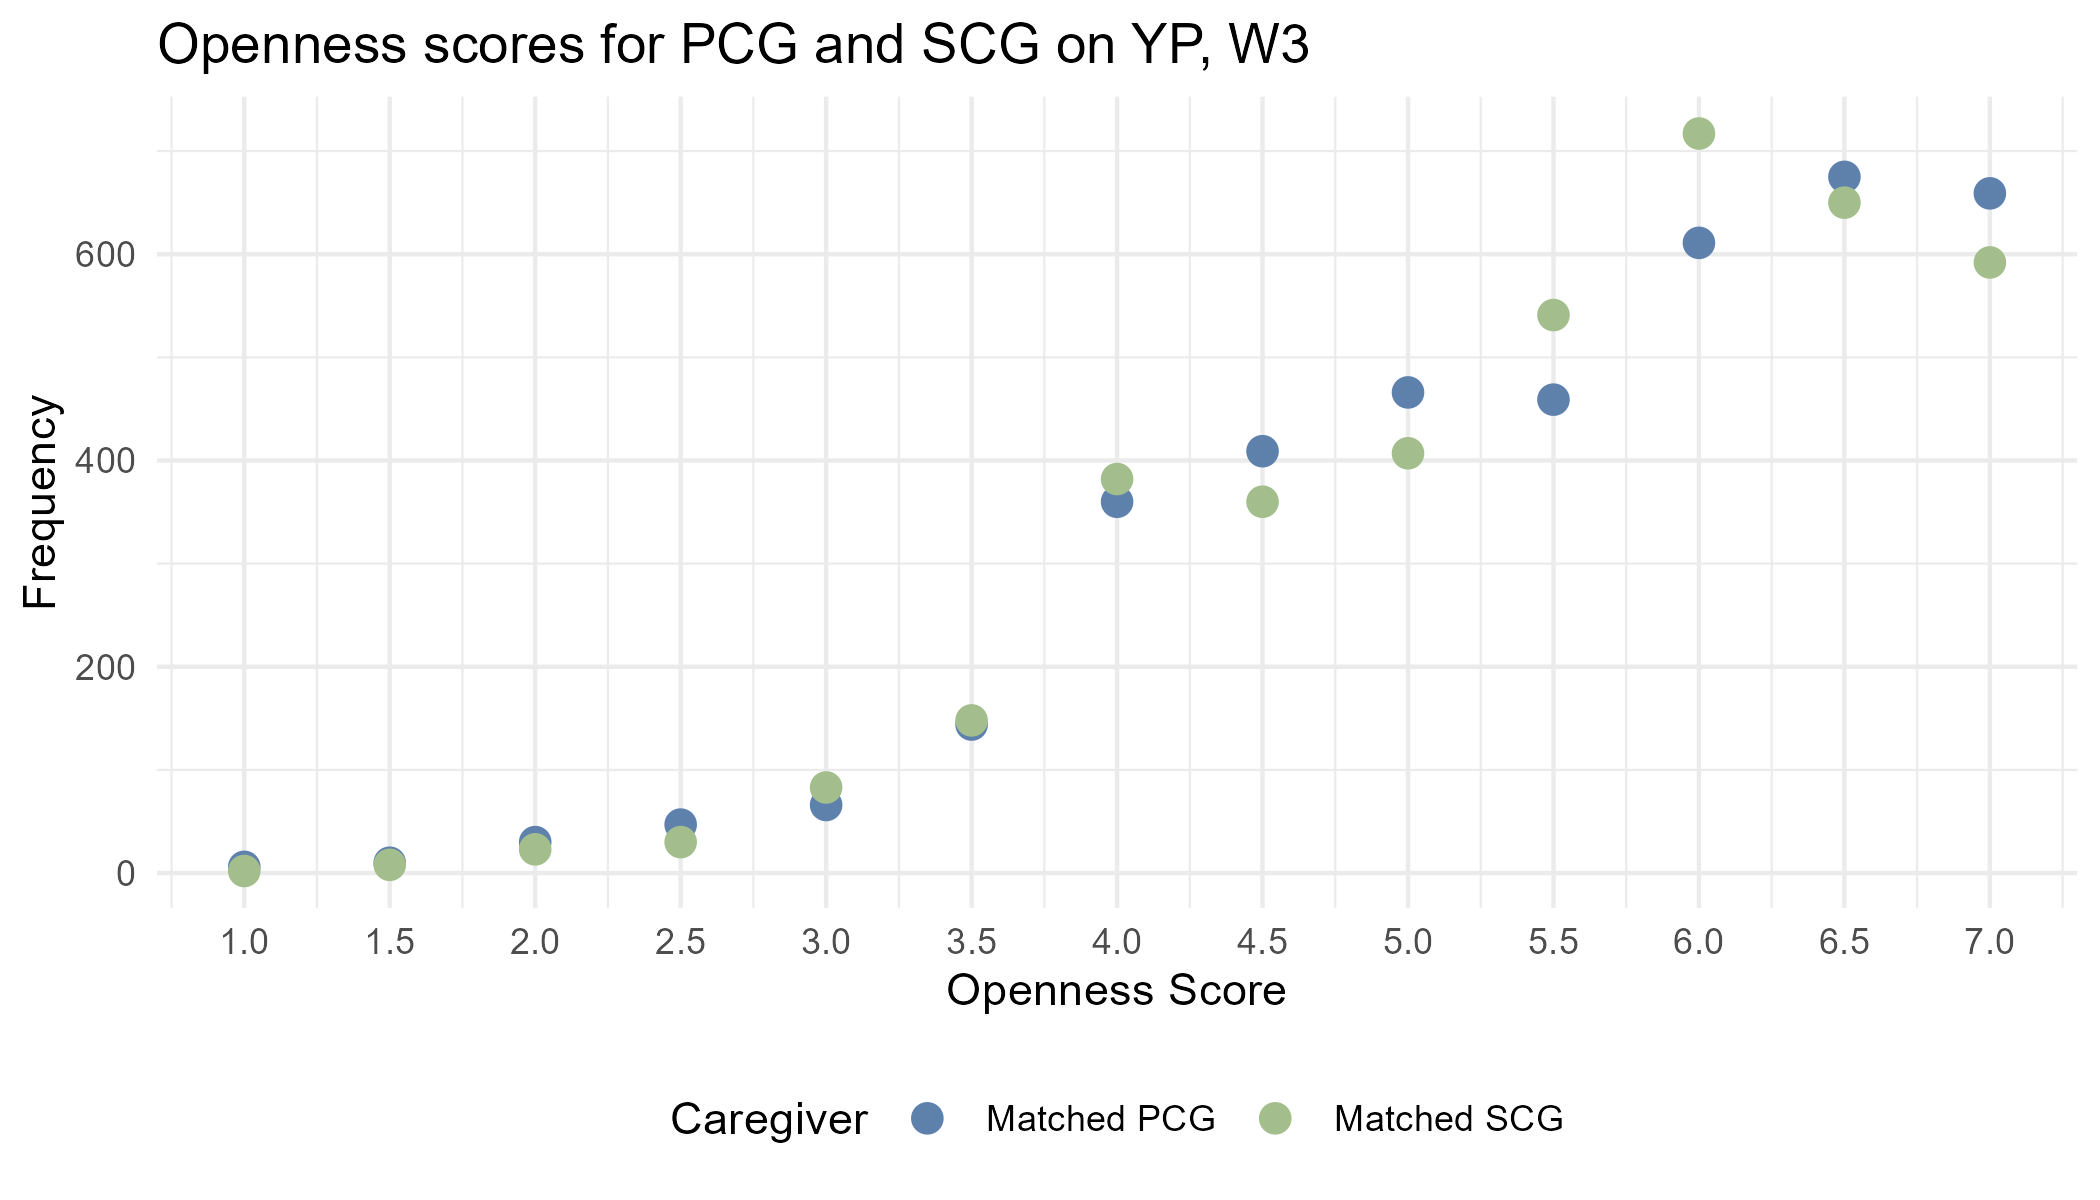
\includegraphics[width=1\linewidth]{Matched Openness by participant w3.jpeg}
    \caption{Frequency of YP's Openness scores reported by PCG and SCG in wave 3 (matched)}
    \label{}
\end{figure}

\begin{figure}[htbp] 
    \centering
    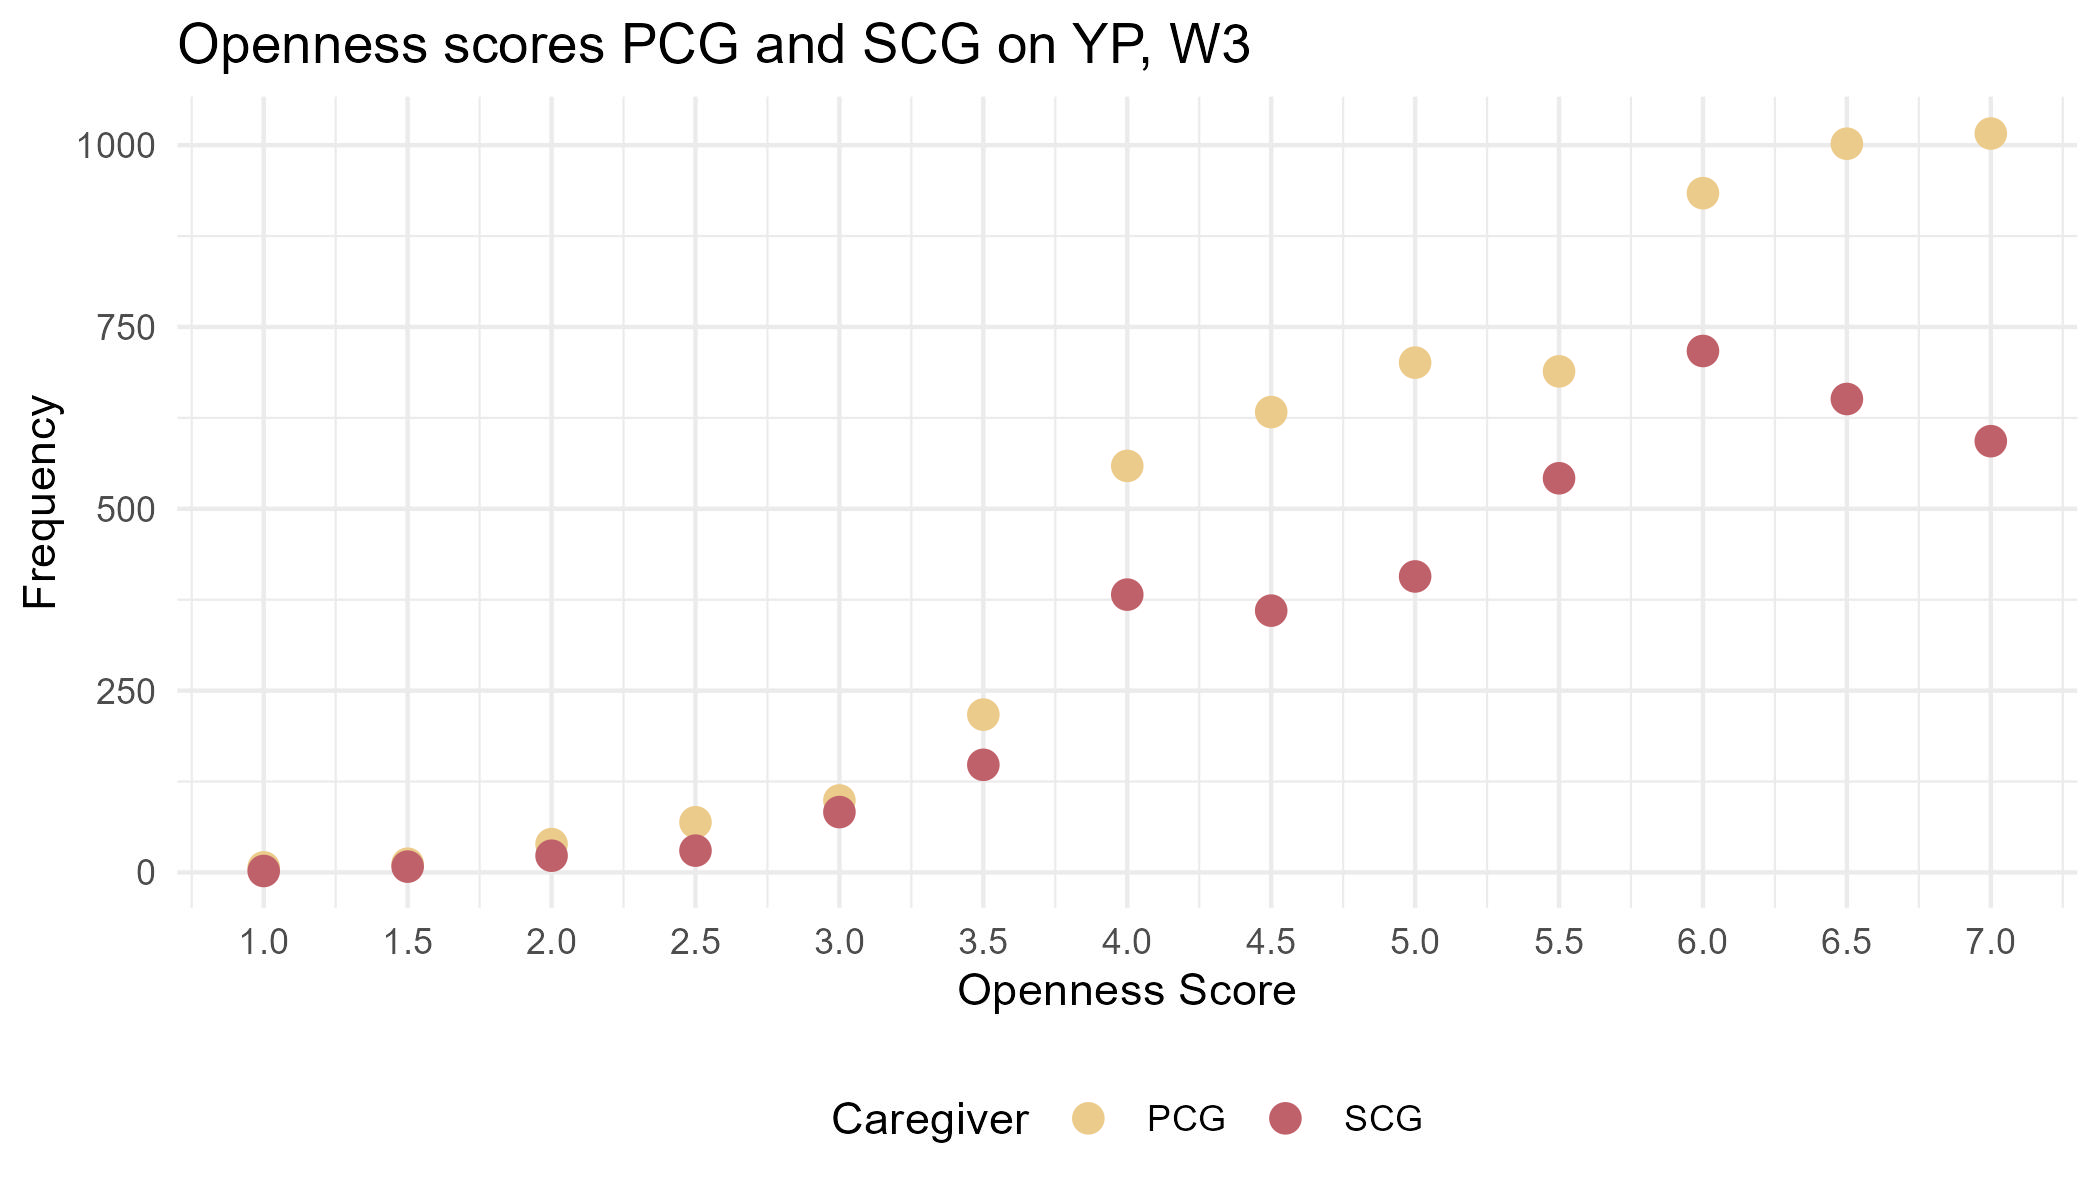
\includegraphics[width=1\linewidth]{Frequency of Openness by participant w3.jpeg}
    \caption{Frequency of YP's Openness scores reported by PCG and SCG in wave 3 (not matched}
    \label{}
\end{figure}

\begin{figure}[htbp] 
    \centering
    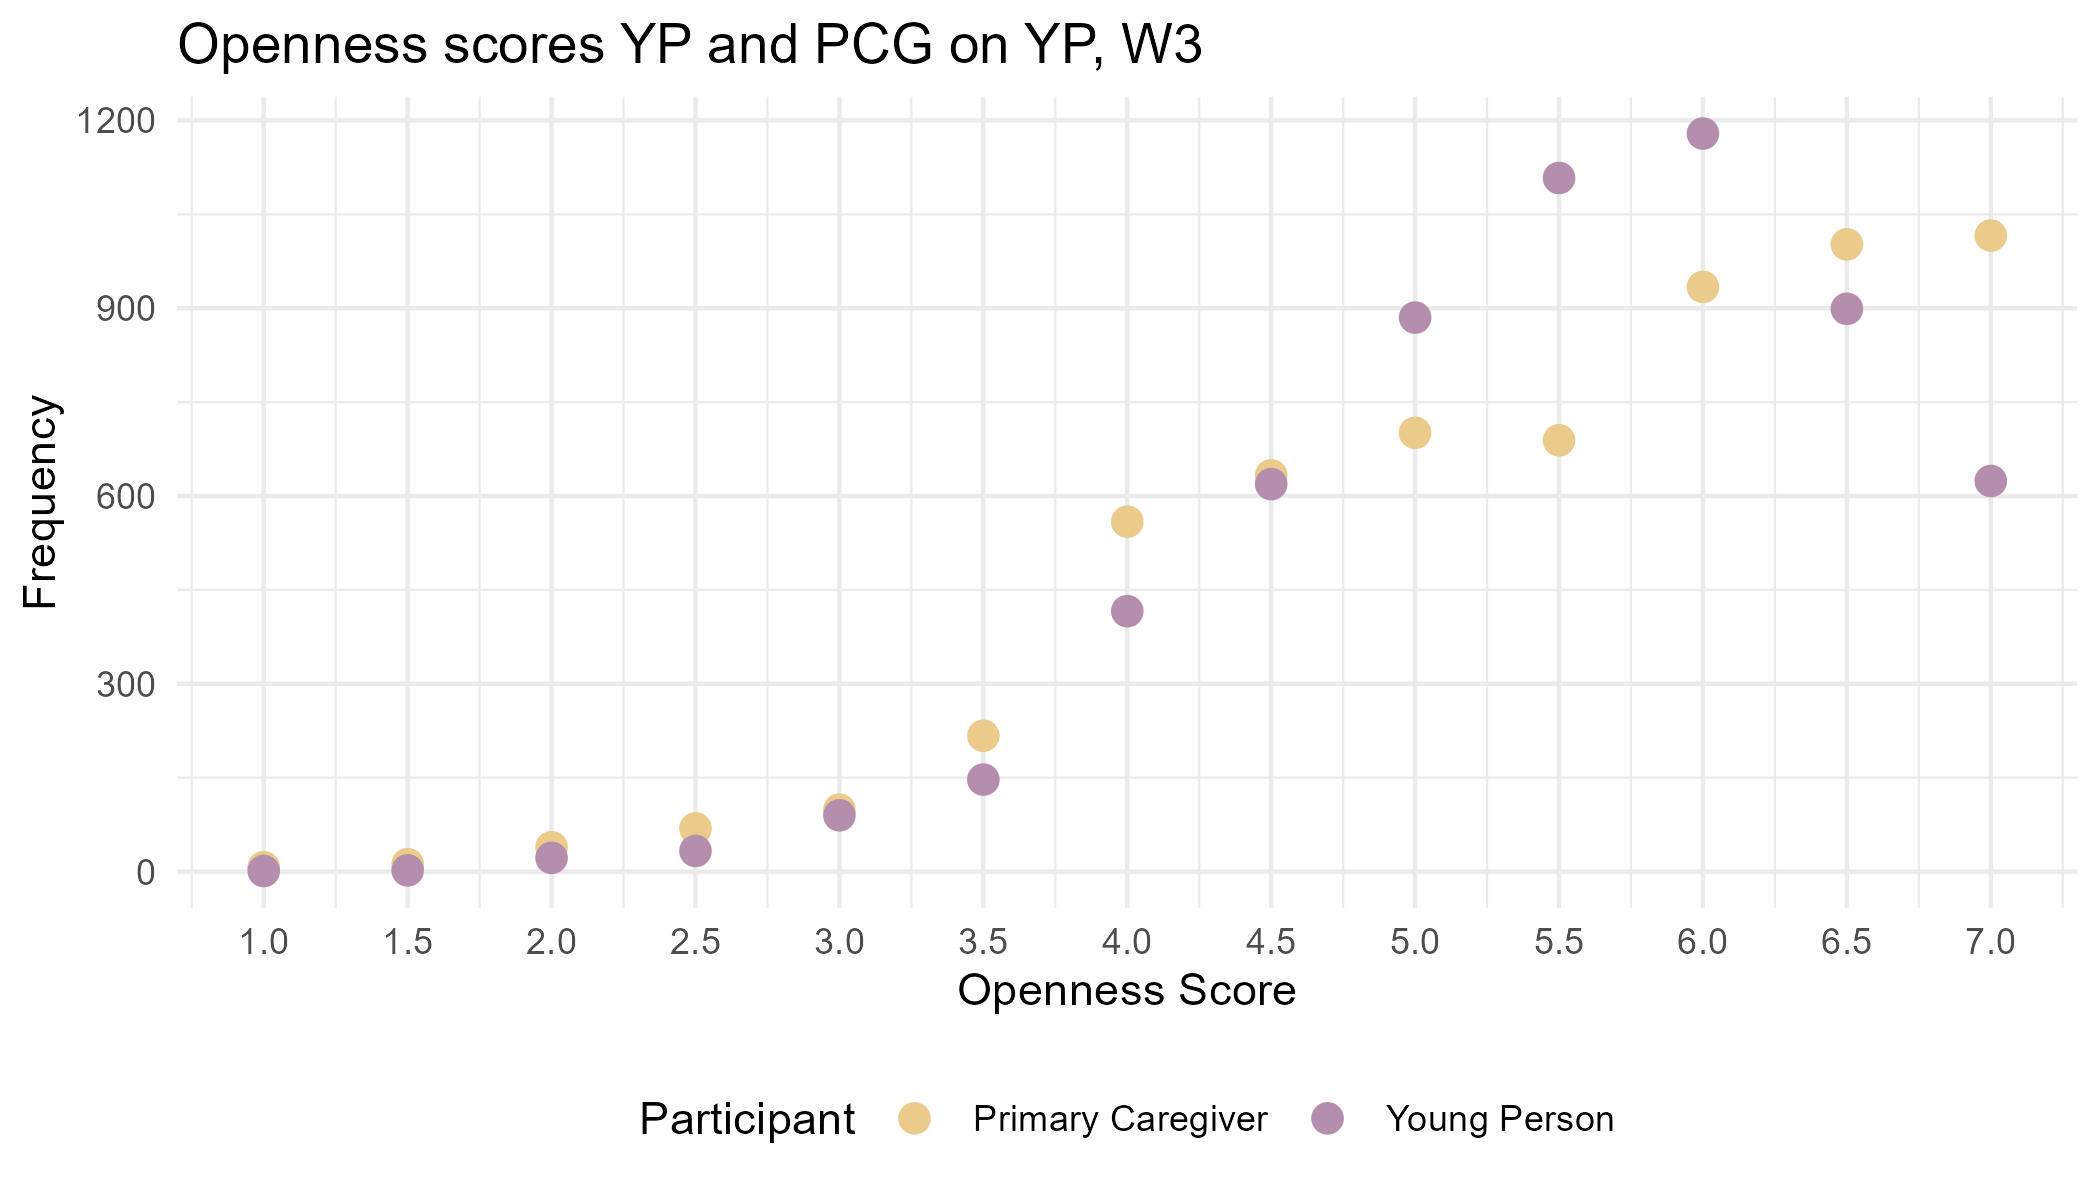
\includegraphics[width=1\linewidth]{Frequency of Openness by participant w3a.jpeg}
    \caption{Frequency of YP's Openness scores reported by YP and PCG in wave 3}
    \label{}
\end{figure}

\clearpage
\subsection{JC grades}
\begin{figure}[htbp] 
    \centering
    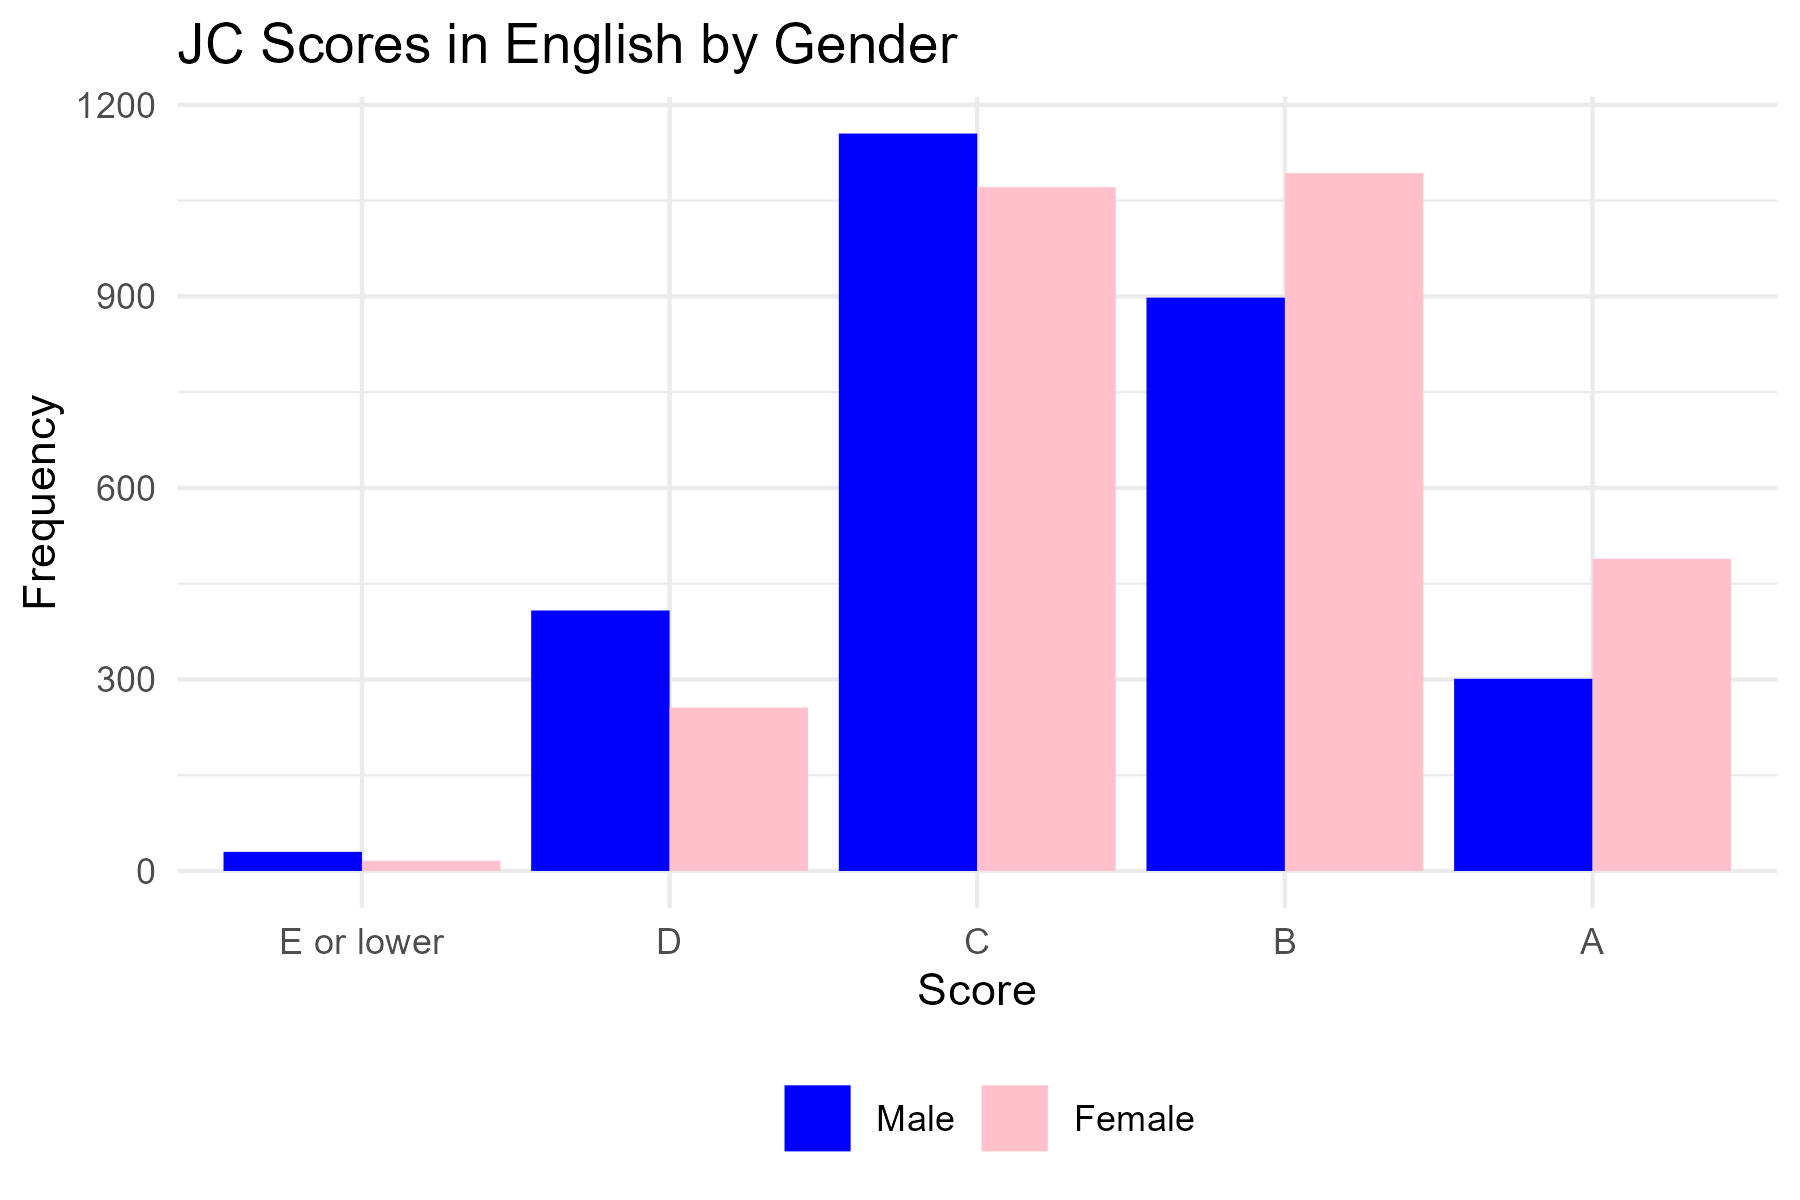
\includegraphics[width=1\linewidth]{Frequency of Test Scores in English by Gender.jpeg}
    \caption{Frequency of Test Scores in English, by gender}
    \label{}
\end{figure}

\begin{figure}[htbp] 
    \centering
    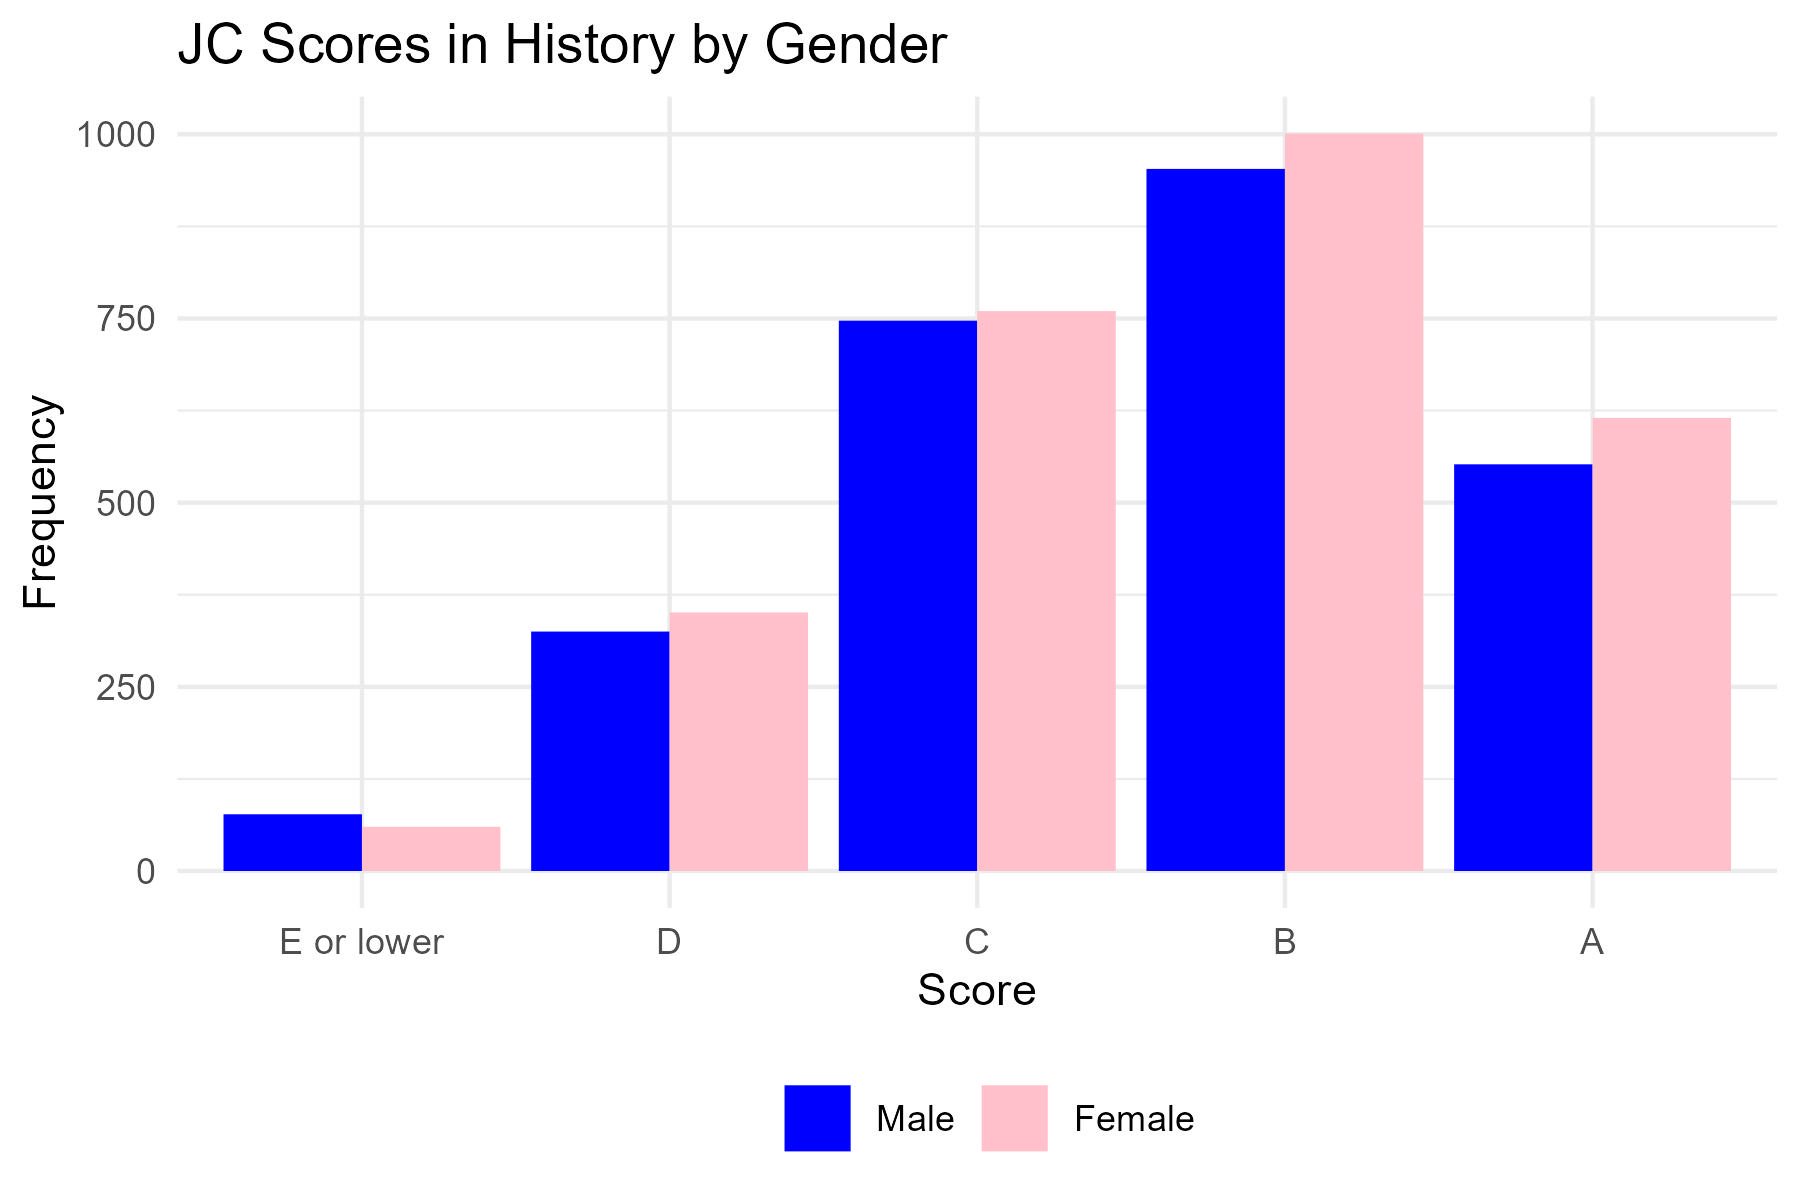
\includegraphics[width=1\linewidth]{Frequency of Test Scores in History by Gender.jpeg}
    \caption{Frequency of Test Scores in History, by gender}
    \label{}
\end{figure}


\begin{figure}[htbp] 
    \centering
    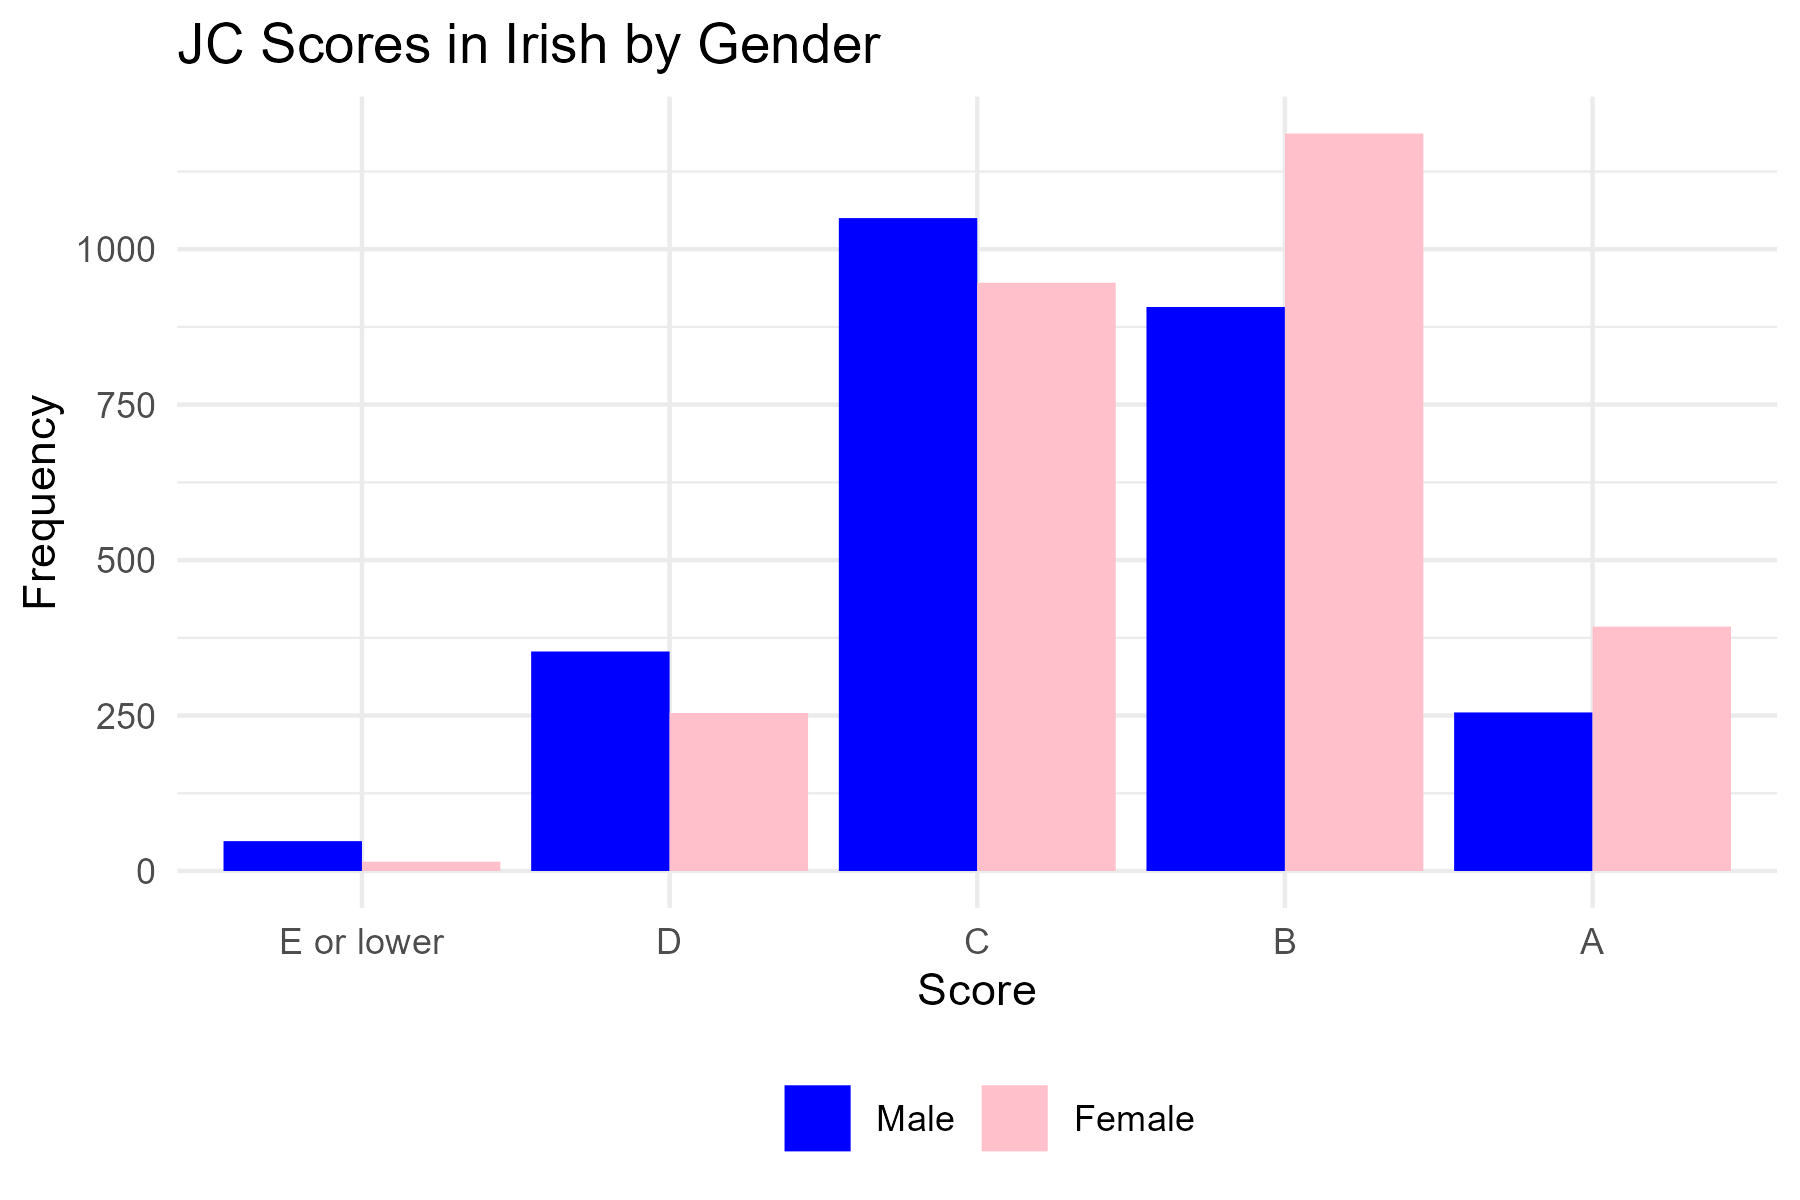
\includegraphics[width=1\linewidth]{Frequency of Test Scores in Irish by Gender.jpeg}
    \caption{Frequency of Test Scores in Irish, by gender}
    \label{}
\end{figure}

\begin{figure}[htbp] 
    \centering
    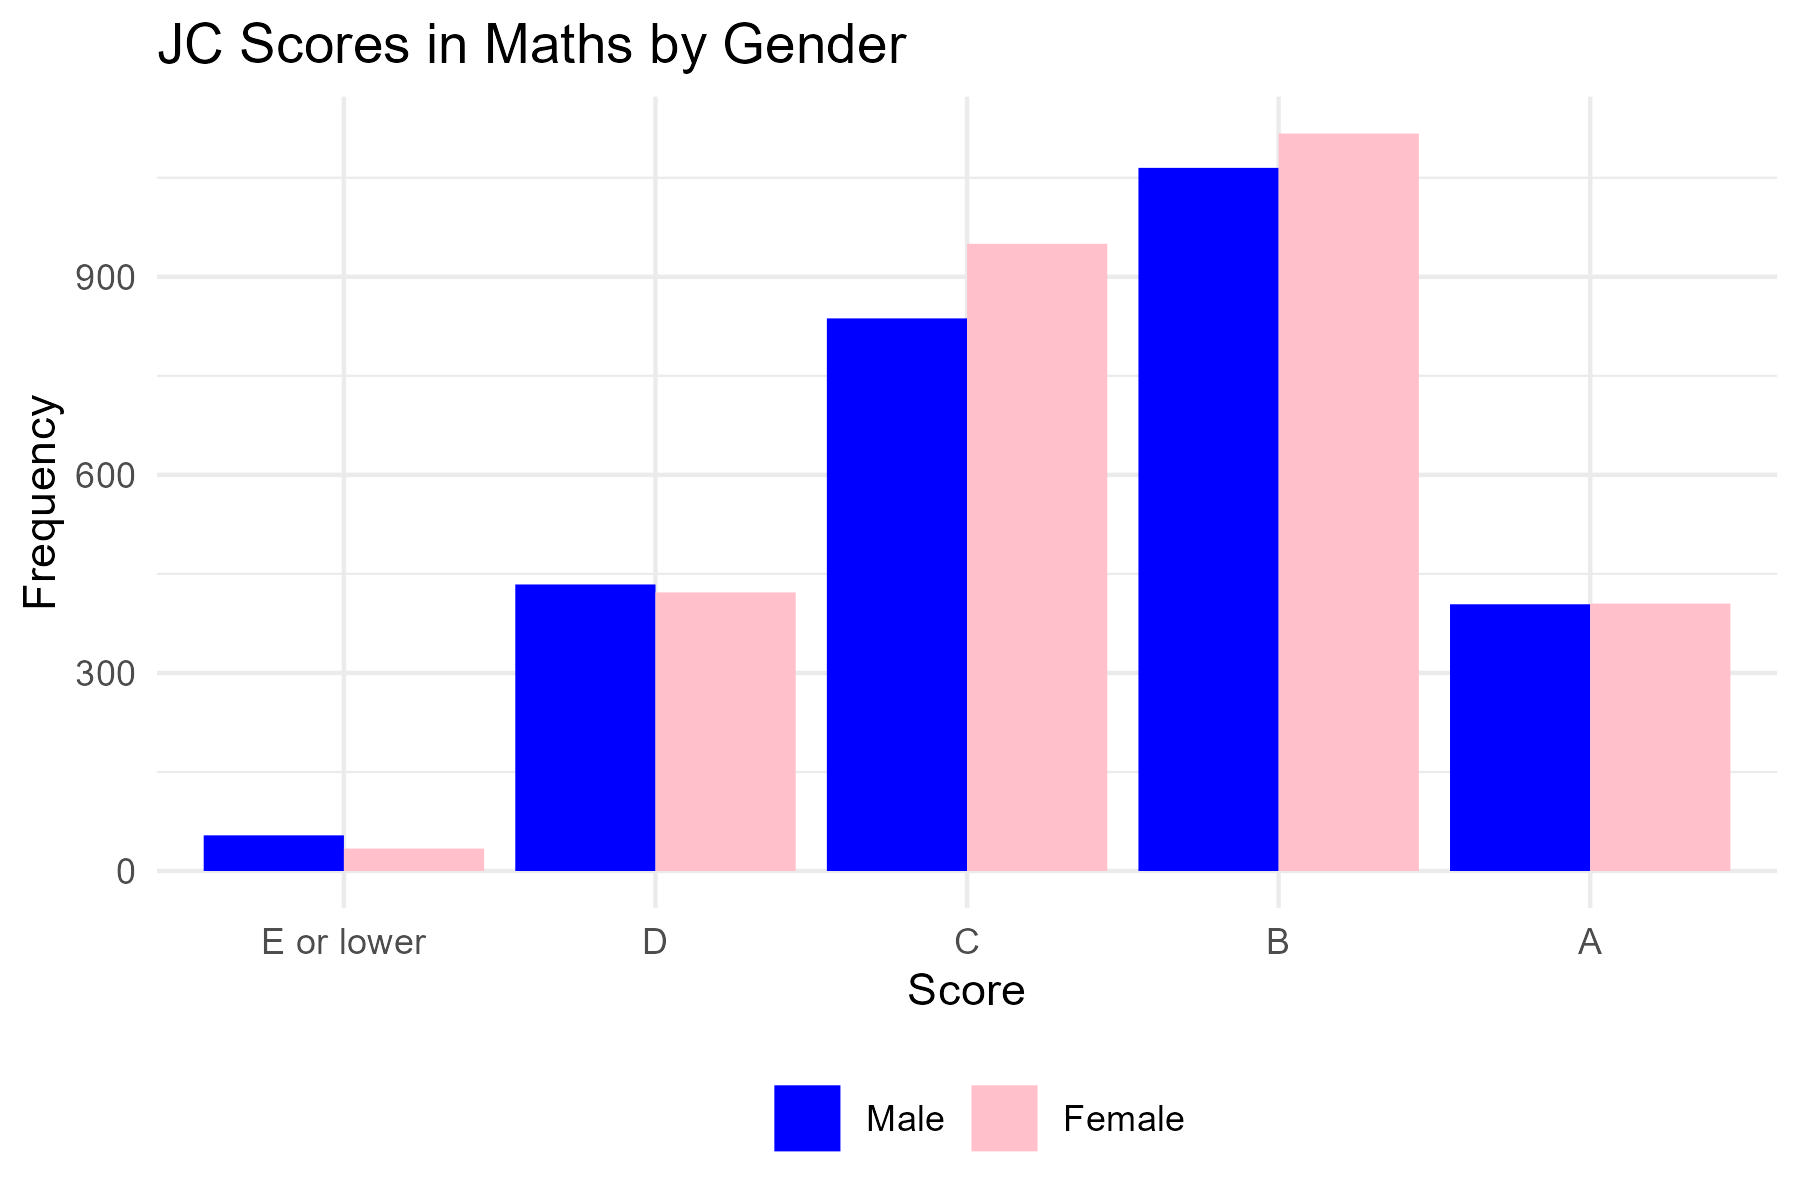
\includegraphics[width=1\linewidth]{Frequency of Test Scores in Maths by Gender.jpeg}
    \caption{Frequency of Test Scores in Maths, by gender}
    \label{}
\end{figure}

\begin{figure}[htbp] 
    \centering
    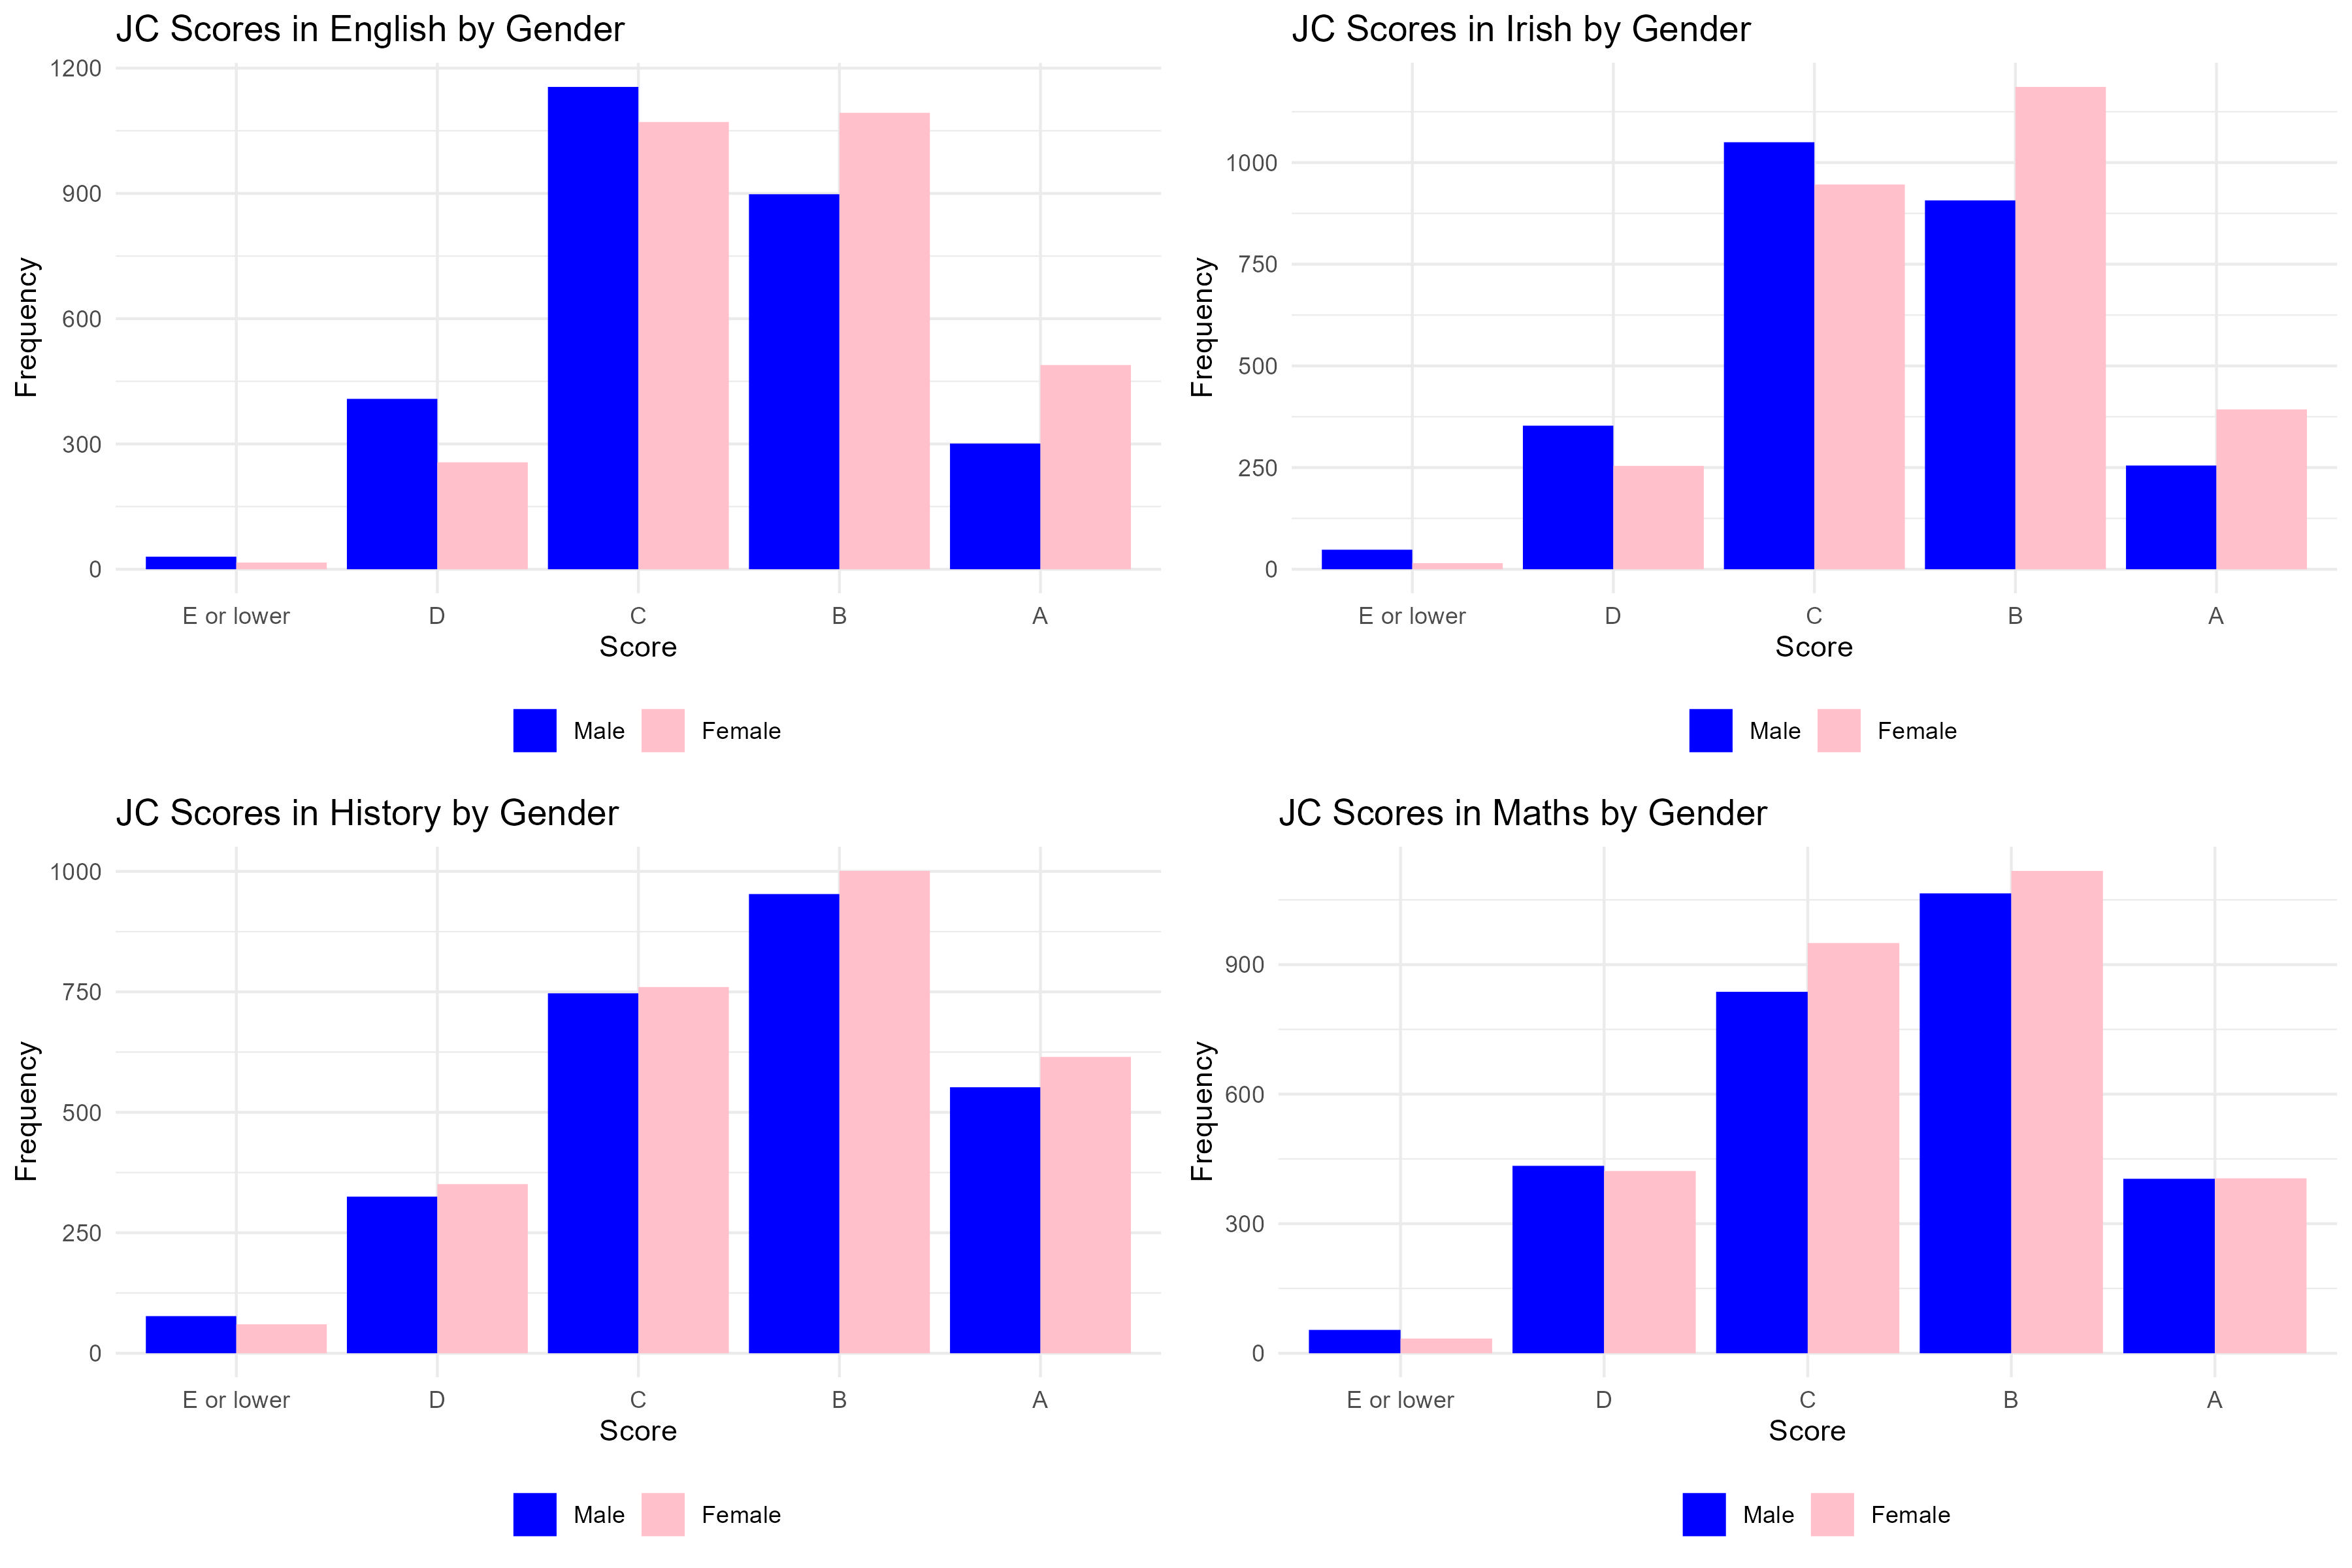
\includegraphics[width=1\linewidth]{Frequency of Test Scores by Gender side by side.jpeg}
    \caption{Frequency of Test Scores for the four subjects, by gender}
    \label{}
\end{figure}

\clearpage
\subsection{Questions}
\begin{figure}[htbp] 
    \centering
    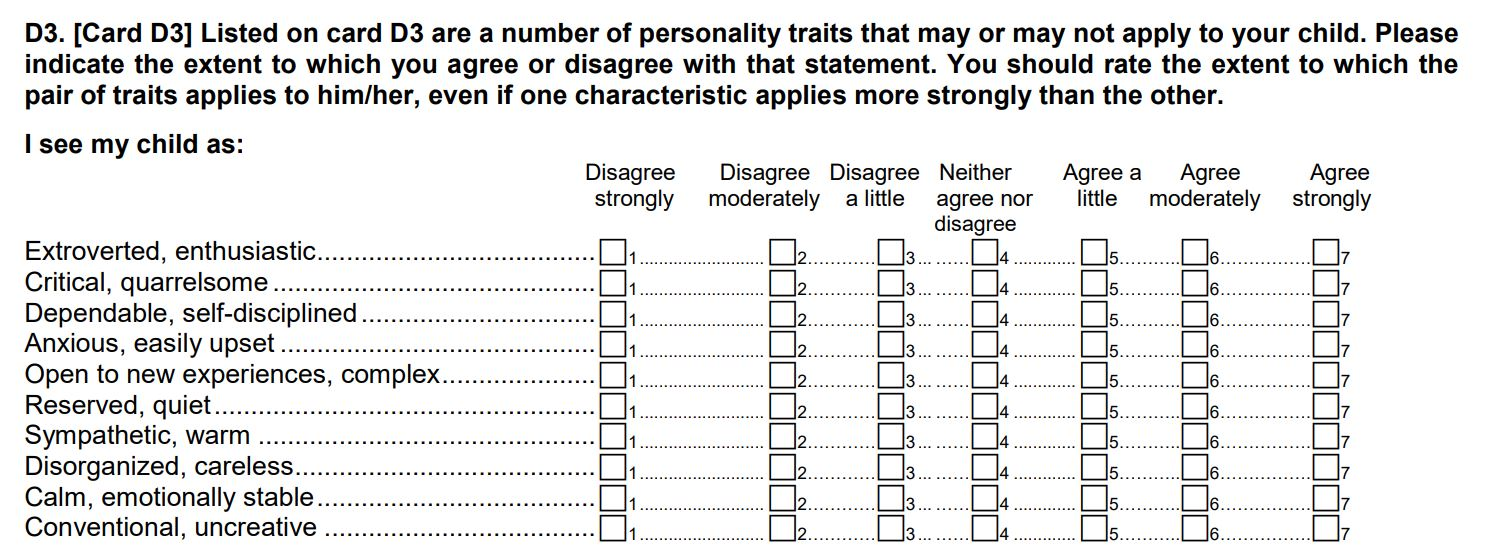
\includegraphics[width=1\linewidth]{TIPI_PCG.JPG}
    \caption{TIPI scores}
    \label{}
\end{figure}

\begin{figure}[htbp] 
    \centering
    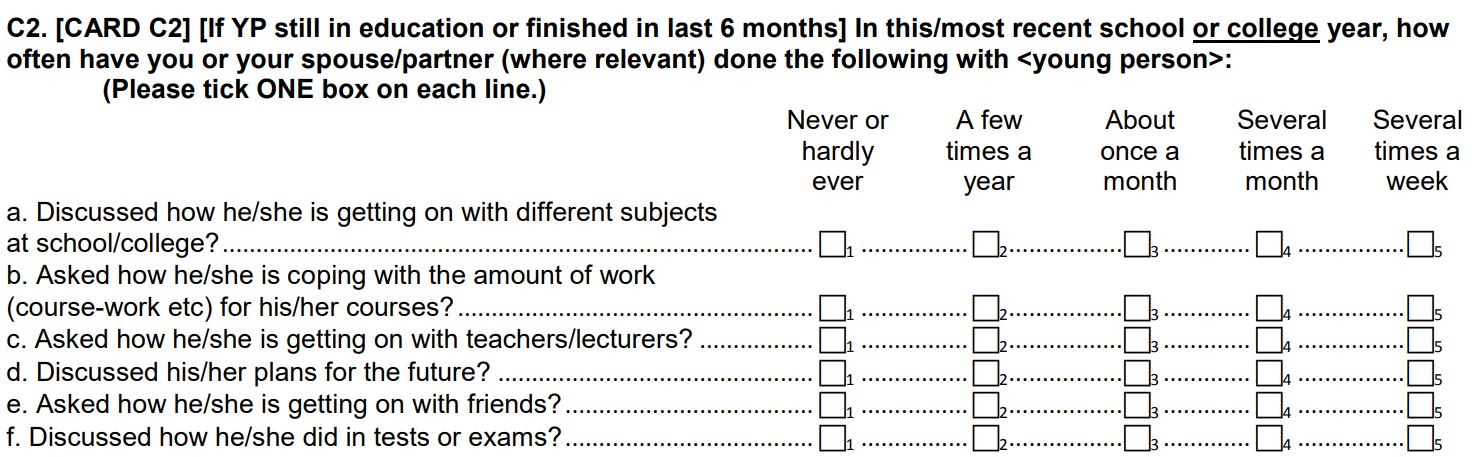
\includegraphics[width=1\linewidth]{PI.JPG}
    \caption{Parental involvement}
    \label{}
\end{figure}


\end{document}